\documentclass{ieeeaccess}
\usepackage{cite}
\usepackage{amsmath,amssymb,amsfonts}
\usepackage{algorithmic}
\usepackage{graphicx}
\usepackage{textcomp}
\usepackage{booktabs}
\usepackage{multirow}
\usepackage{url}
\usepackage{bm}

\graphicspath{{figures/}{./}{../figures/}}

\def\BibTeX{{\rm B\kern-.05em{\sc i\kern-.025em b}\kern-.08em
    T\kern-.1667em\lower.7ex\hbox{E}\kern-.125emX}}

\begin{document}
\history{Date of publication March 2026, date of current version March 2026.}
\doi{10.1109/ACCESS.2026.DOI\_PREPRINT\_PDI\_QML}

\title{Quantum-Enhanced Vision Framework for Sunflower Pollen Deficiency Estimation: A Comparative Benchmark of Classical Baselines and Variational Quantum State Encodings}

\author{\uppercase{Ramit Bose}\authorrefmark{1}, \IEEEmembership{Student Member, IEEE}, AND \uppercase{Samriddhi Sarkar}\authorrefmark{1}, \IEEEmembership{Senior Member, IEEE}}

\address[1]{Department of Computer Science and Engineering, School of Computer Science and Engineering, Vellore Institute of Technology, Vellore 632014, Tamil Nadu, India (e-mail: ramit.bose2024@vitstudent.ac.in, samriddhi.sarkar@vit.ac.in)}

\tfootnote{This work was supported by institutional research facilities at the School of Computer Science and Engineering, Vellore Institute of Technology.}

\markboth
{Bose and Sarkar: Quantum-Enhanced Vision Framework for Sunflower Pollen Deficiency Estimation}
{Bose and Sarkar: Quantum-Enhanced Vision Framework for Sunflower Pollen Deficiency Estimation}

\corresp{Corresponding author: Ramit Bose (e-mail: ramit.bose2024@vitstudent.ac.in).}

\begin{abstract}
In hybrid sunflower (\textit{Helianthus annuus} L.) seed production, rapid assessment of pollination adequacy is critical to preventing floret sterility and yield loss. Conventional field evaluations rely on destructive microscopic pollen assays, while existing computer vision tools merely detect capitulum presence without appraising floret fertilization viability. This paper presents an end-to-end vision pipeline and empirical quantum machine learning (QML) benchmark for estimating an auditable Pollen Deficiency Index (PDI) proxy. From 5,351 real-world floral images across five developmental stages, a stratified cohort of 1,500 images undergoes CIE-$L^*a^*b^*$ color space decoupling, lightness-channel CLAHE, and bilateral filtering. A dual-stage GrabCut and $K$-means ($k=3$) segmentation algorithm isolates the central tubular floret disc, extracting 31 multi-domain non-circular morphological, spectral, and GLCM textural descriptors. Classical baselines achieve up to 93.94\% test accuracy across Logistic Regression, XGBoost, and Multi-Layer Perceptron. To benchmark near-term quantum utility, two 6-qubit Variational Quantum Classifiers (VQCs) are evaluated: Method~1 (6-D PCA with Pauli-$Y$ angle encoding) versus Method~2 (zero-dimensionality-reduction amplitude encoding in a 64-dimensional Hilbert space). Method~2 decisively outperforms Method~1 across all metrics, achieving 84.85\% versus 81.82\% accuracy, 0.9522 versus 0.9338 ROC-AUC, and a 25\% reduction in false-positive errors. Furthermore, the quantum circuit utilizes only 38 trainable parameters (a 99.1\% reduction versus classical neural networks) and demonstrates noise robustness up to depolarizing probability $p = 0.05$.
\end{abstract}

\begin{keywords}
Computer vision, digital image processing, \textit{Helianthus annuus}, inflorescence phenotyping, parameter parsimony, parameterized quantum circuits, pollen deficiency index, precision agriculture, quantum amplitude encoding, variational quantum classifier.
\end{keywords}

\titlepgskip=-15pt
\maketitle

\section{Introduction}
\label{sec:introduction}
\PARstart{I}{n} industrial hybrid seed production and precision agronomy, the commercial sunflower (\textit{Helianthus annuus} L.) occupies a preeminent position as a high-value oilseed crop worldwide \cite{jing2024sunflower}. Unlike self-fertile cereal crops such as wheat or rice, the composite sunflower inflorescence (the capitulum) exhibits pronounced protandrous dichogamy and sporophytic self-incompatibility \cite{aslan2023sunflower}. The thousands of individual hermaphroditic tubular florets comprising the central floral disc mature centripetally---from the outer margin inward toward the center over an anthesis period of 5 to 10 days \cite{mallinger2015species}. During anthesis, stigmata depend primarily upon external biotic pollination vectors, predominantly honey bees (\textit{Apis mellifera}) and wild solitary bees, to transfer viable pollen from pollen-shedding florets to receptive bifid stigmas \cite{rice2024uav}.

When environmental stress (such as extreme heat, drought, or micronutrient boron deficiency) suppresses pollen dehiscence, or when pollinator activity is insufficient during the receptive stigma window, floret fertilization fails. This leads to empty achenes, unfulfilled central disc whorls, and hollow seed hulls---a syndrome agronomically defined as pollen deficiency \cite{iamchuen2026automated}. In severe cases, seed-set rates drop below 40\%, inflicting severe economic yield losses. Traditional crop inspection relies on manual, destructive field sampling: agronomists pluck capitula, extract pollen grains with organic solvents, and perform microscopic hemocytometer grain counts and viability staining \cite{haralick1973textural}. Such manual methods are inherently destructive, spatially sparse, and prohibitively labor-intensive for commercial field scales.

Recent advances in remote sensing and optical phenotyping have introduced computer vision tools for sunflower monitoring. Deep learning architectures, such as Sunflower-YOLO \cite{jing2024sunflower} and Sunpheno \cite{luoni2024sunpheno}, successfully detect sunflower capitula in UAV imagery and categorize gross phenological growth stages. However, a critical scientific gap persists: existing vision frameworks identify whether a flower is blooming, but completely fail to quantify whether the blooming flower is adequately pollinated. Flower bloom is an optical prerequisite, but not a biological guarantee, of fertilization. Unpollinated florets remain visually present on the capitulum for days, disguising reproductive failure under standard aerial detectors \cite{smith2025remote}.

Concurrently, the emergence of Noisy Intermediate-Scale Quantum (NISQ) computing has catalyzed interest in Quantum Machine Learning (QML) for agricultural and environmental image processing \cite{biamonte2017quantum, henderson2020quanvolutional, schuld2020circuit}. Parameterized Quantum Circuits (PQCs) and Variational Quantum Classifiers (VQCs) offer theoretical mechanisms for mapping feature vectors into exponentially large complex Hilbert spaces ($\mathcal{H} \cong \mathbb{C}^{2^n}$) using logarithmic physical qubit counts ($n = \lceil \log_2(D) \rceil$) \cite{schuld2019quantum}. Furthermore, quantum state superpositions and entangling unitaries can uncover complex cross-feature interactions with exceptional parameter parsimony, using orders of magnitude fewer trainable weights than deep classical convolutional neural networks \cite{cerezo2021variational}. However, the application of QML to plant phenotyping remains severely constrained by the quantum state preparation bottleneck: classical data encoding schemes often suffer from extensive information loss or excessive circuit depth on NISQ simulators \cite{schuld2021supervised}.

To address these intertwined challenges, this investigation develops an auditable, reproducible vision pipeline and a rigorous hybrid quantum-classical benchmark for estimating an agronomic Pollen Deficiency Index (PDI) proxy. Based on the project foundations and literature review synthesized in project review documentation \cite{bose2026progress}, this paper resolves eight distinct research gaps:
\begin{enumerate}
    \item Absence of an image-derived botanical Pollen Deficiency Index (PDI) tailored for sunflower inflorescences.
    \item Disconnect between capitulum-level flowering presence and localized floret fertilization viability.
    \item Lack of standardized Digital Image Processing (DIP) workflows combining illumination-invariant color decoupling with multi-domain feature engineering.
    \item Inattention to sub-capitulum disc-to-flower geometric ratios during anthesis in machine learning schemas.
    \item Complete absence of quantum machine learning formulations applied to crop reproductive viability estimation.
    \item Scarcity of unmanipulated, head-to-head empirical comparisons between classical and quantum algorithms on identical feature sets.
    \item Lack of empirical quantum depolarizing noise tolerance profiling on real botanical feature distributions.
    \item Scarcity of transparent, laptop-feasible edge implementations that operate without high-performance computing clusters.
\end{enumerate}

\section{Related Work \& Theoretical Foundations}
\label{sec:related_work}

\subsection{Optical Phenotyping in Sunflower Crops}
The application of optical computer vision to sunflower phenomics has expanded rapidly over the past five years, driven by the need for high-throughput crop monitoring \cite{jing2024sunflower}. Jing et al. \cite{jing2024sunflower} developed Sunflower-YOLO, an edge-optimized detector based on YOLOv7-tiny, evaluated on 1,539 UAV remote sensing images containing 75,846 annotated capitula across diverse phenological phases. While achieving an impressive mean average precision (mAP@0.5) of $\sim$93\%, their model operates strictly as a bounding-box object detector; it does not generate pixel-level segmentation masks of floral discs nor estimate floret-level fertilization status.

Yildirim, Colkesen, and Sefercik \cite{yildirim2026evaluating} investigated semantic segmentation architectures, comparing transformer-based (SegFormer) and convolutional models for identifying sunflower inflorescences in aerial surveys. Their findings demonstrated that attention mechanisms better handle boundary ambiguities between yellow ray petals and background weeds, achieving an intersection-over-union (mIoU) exceeding 85\%. Similarly, Luoni et al. \cite{luoni2024sunpheno} introduced Sunpheno, a convolutional neural network designed to categorize five developmental phases from ground-level RGB images. Although Sunpheno demonstrated the viability of automated growth-stage classification, the authors noted that visual stage classification alone cannot infer whether anthers have released viable pollen or whether stigmata have withered prematurely.

\subsection{Quantum Machine Learning for Vision and NISQ Paradigms}
Quantum Machine Learning seeks to harness quantum mechanical phenomena---namely superposition, quantum interference, and entanglement---to enhance statistical learning \cite{biamonte2017quantum, schuld2019quantum}. Schuld and Killoran \cite{schuld2019quantum} established that parameterized quantum circuits act as linear models operating within a reproducing kernel Hilbert space defined by the quantum state preparation routine. Biamonte et al. \cite{biamonte2017quantum} and Mitarai et al. \cite{mitarai2018quantum} formalized quantum circuit learning, wherein classical optimization algorithms iteratively adjust gate rotation angles to minimize a cost function.

In image classification, Henderson et al. \cite{henderson2020quanvolutional} introduced ``Quanvolutional Neural Networks'', wherein small quantum circuits act as localized feature kernels scanning across pixel matrices. Long et al. \cite{long2025hybrid} proposed a three-stage hybrid quantum-classical-quantum convolutional architecture combining quantum filters, shallow classical CNN layers, and a variational QNN classifier, demonstrating resilient convergence under depolarizing noise on benchmark datasets. Daka et al. \cite{daka2026novel} formulated a colour-aware quantum convolutional network utilizing problem-specific RGB block-matrix encodings for pixelated images, reporting notable small-sample generalization advantages over classical counterparts.

\subsection{Feature Encoding Paradigms in Quantum Circuits}
A foundational decision in designing any variational quantum classifier is the quantum feature map \cite{schuld2021supervised, lloyd2013quantum}. In the NISQ regime, two primary encoding paradigms predominate: Angle Encoding and Amplitude Encoding. In Angle Encoding, $D$ classical continuous variables $\mathbf{x} = [x_1, \dots, x_D]^T$ are mapped to rotation angles of single-qubit gates, typically Pauli-$Y$ or Pauli-$Z$ rotations, operating on $D$ physical qubits:
\begin{equation}
    |\psi_{\text{angle}}(\mathbf{x})\rangle = \bigotimes_{j=0}^{D-1} RY(x_j)|0\rangle = \bigotimes_{j=0}^{D-1} \left[ \cos\left(\frac{x_j}{2}\right)|0\rangle + \sin\left(\frac{x_j}{2}\right)|1\rangle \right].
    \label{eq:angle_encoding}
\end{equation}
While angle encoding requires circuit depth $\mathcal{O}(1)$ for state preparation and avoids complex multi-qubit gate decompositions, it scales linearly with feature dimensionality: representing $D$ features demands $D$ physical qubits \cite{lloyd2013quantum}. Consequently, when operating under a strict 6-qubit hardware budget, high-dimensional datasets must undergo aggressive classical dimensionality reduction (such as PCA), discarding potentially discriminative feature variance \cite{bose2026progress}.

Conversely, Quantum Amplitude Encoding embeds a normalized classical vector $\mathbf{x} \in \mathbb{R}^{2^n}$ directly into the probability amplitudes of an $n$-qubit quantum state:
\begin{equation}
    |\psi_{\text{amp}}(\mathbf{x})\rangle = \sum_{i=0}^{2^n - 1} c_i |i\rangle, \quad \text{where} \quad \sum_{i=0}^{2^n - 1} |c_i|^2 = 1.0.
    \label{eq:amplitude_encoding}
\end{equation}
Amplitude encoding provides an exponential state capacity, allowing an $n$-qubit quantum system to represent $2^n$ continuous features \cite{schuld2021supervised}. For a 31-dimensional botanical feature vector, $n = \lceil \log_2(31) \rceil = 6$ physical qubits provide $2^6 = 64$ basis states, enabling the direct embedding of all 31 features without classical PCA reduction. Although arbitrary amplitude state preparation on physical NISQ processors requires $\mathcal{O}(2^n)$ multi-controlled entangling gates \cite{lloyd2013quantum}, its simulated mathematical expressivity provides an ideal testbed for evaluating whether preserving full botanical feature variance in Hilbert space surpasses classical linear compression.

\section{System Architecture \& Methodology}
\label{sec:methodology}

\subsection{Dataset Stratification and Agronomic Categorization}
The experimental dataset consists of 5,351 high-resolution, real-world ground-level sunflower photographs curated to encompass the complete botanical developmental spectrum of \textit{Helianthus annuus}. The images are categorized into five mutually exclusive developmental classes: YoungBud ($N = 1,027$), MatureBud ($N = 1,010$), EarlyBloom ($N = 1,080$), Healthy ($N = 1,204$), and Wilted ($N = 1,039$). Table~\ref{tab:dataset_stratification} summarizes the dataset stratification across all experimental phases.

\begin{table*}[!t]
\caption{Empirical Growth Stage and Dataset Stratification Across Experimental Phases}
\label{tab:dataset_stratification}
\centering
\begin{tabular*}{\textwidth}{@{\extracolsep{\fill}}lcccccc@{}}
\toprule
\textbf{Developmental Class} & \textbf{Total Images} & \textbf{Phase 1 Stratified} & \textbf{Train Split (70\%)} & \textbf{Val Split (15\%)} & \textbf{Test Split (15\%)} & \textbf{Botanical Phenology Description} \\
\midrule
YoungBud   & 1,027 & 300 & 210 & 45 & 45 & Pre-anthesis; capitulum enclosed by green involucral bracts \\
MatureBud  & 1,010 & 300 & 210 & 45 & 45 & Opening bud; yellow ray ligules emerging; disc florets closed \\
EarlyBloom & 1,080 & 300 & 210 & 45 & 45 & Active early anthesis; outer tubular florets actively shedding pollen \\
Healthy    & 1,204 & 300 & 210 & 45 & 45 & Full anthesis; vibrant ray florets; central disc actively receptive \\
Wilted     & 1,039 & 300 & 210 & 45 & 45 & Post-anthesis; senescent ray petals; fertilized ovary maturation \\
\midrule
\textbf{Total / Summary} & \textbf{5,351} & \textbf{1,500} & \textbf{1,050} & \textbf{225} & \textbf{225} & \textbf{Deterministic seed = 42; 100\% reproducible pipeline} \\
\bottomrule
\end{tabular*}
\end{table*}

Detailed description of Table~\ref{tab:dataset_stratification}: Table~\ref{tab:dataset_stratification} establishes the sample distribution across five biological developmental classes. To prevent class imbalance biases, a balanced subset of exactly 300 images per stage (1,500 total) was drawn using a deterministic random seed (seed = 42). This guarantees equal representation of pre-anthesis, anthesis, and post-anthesis floral morphologies during feature extraction. For Phase 2 quantum experiments, an independent, balanced held-out partition of 220 images (110 Low PDI vs. 110 High PDI) was isolated.

\subsection{Digital Image Processing (DIP) and Dual-Stage Segmentation}
In agricultural field photography, uncontrolled ambient illumination, cloud shadows, and background vegetative clutter present severe obstacles to direct feature extraction. The pipeline implements a structured Digital Image Processing (DIP) workflow, as visualized in full page width in Fig.~\ref{fig:pipeline}.

\begin{figure*}[!t]
\centering
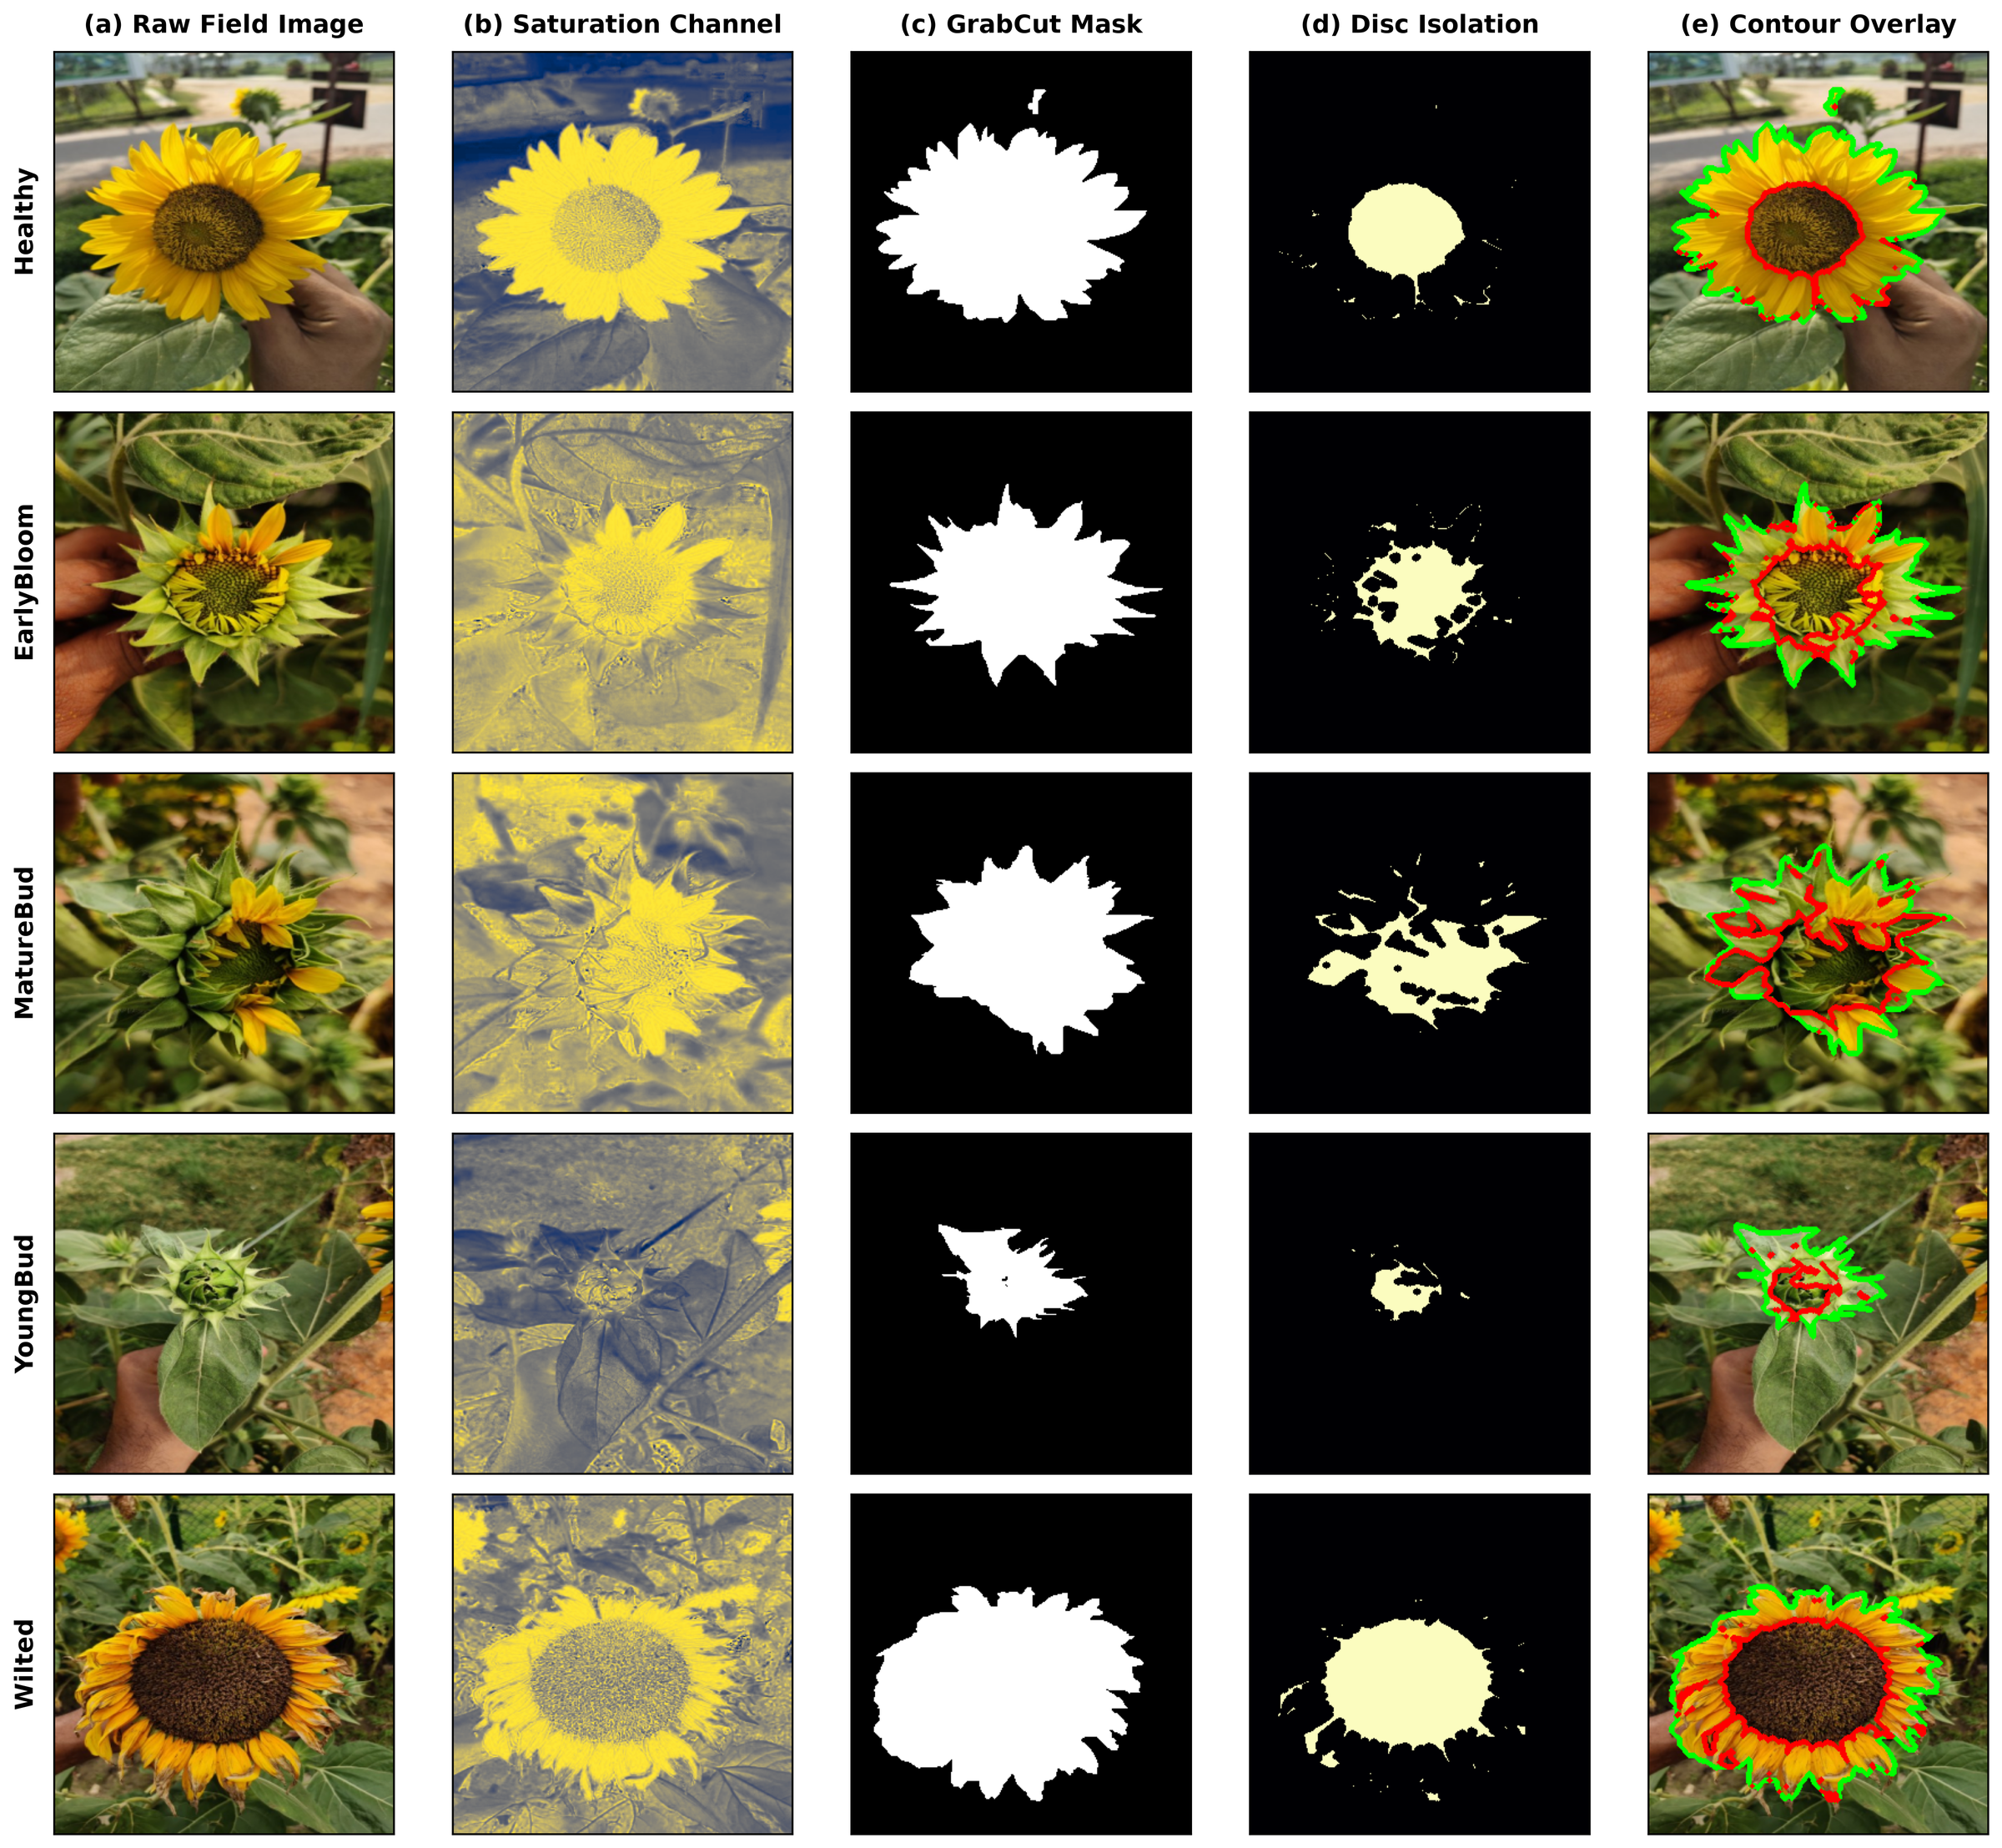
\includegraphics[width=0.98\textwidth]{Fig1_image_segmentation_pipeline.png}
\caption{End-to-end Digital Image Processing (DIP) and dual-stage segmentation pipeline across five growth stages: (a) Input raw image, (b) CIE-$L^*a^*b^*$ conversion and lightness-channel CLAHE, (c) Bilateral edge-preserving filtering, (d) GrabCut flower isolation, (e) $K$-means ($k=3$) central floret disc extraction, and (f) Multi-domain mask overlay.}
\label{fig:pipeline}
\end{figure*}

Detailed description of Fig.~\ref{fig:pipeline}: In step (a), the raw field image shows uneven direct solar illumination and strong background leaf clutter. In step (b), the image is transformed to CIE-$L^*a^*b^*$ space, and CLAHE equalizes the $L^*$ channel using an $8 \times 8$ tile grid with clipping threshold $\beta = 2.0$, revealing subtle floret textures in shaded floral regions. In step (c), bilateral filtering smooths high-frequency soil clutter while preserving petal edges. Step (d) displays the GrabCut segmentation mask, which isolates the complete flower head (foreground ratio 0.08 to 0.47). Step (e) presents the darkest $K$-means cluster ($k=3$), cleanly segmenting the central tubular floret disc (disc ratio 0.12 to 0.21). Finally, step (f) shows the composite morphological contour overlay.

The mathematical formulation of the DIP workflow proceeds as follows:
1) \textit{Color Space Decoupling \& CLAHE}: Raw RGB values are converted to CIE-$L^*a^*b^*$ coordinates via non-linear sRGB transformations using a D65 white point reference. The lightness channel $L^* \in [0, 100]$ is decoupled from chromatic channels $a^*$ and $b^*$. Contrast Limited Adaptive Histogram Equalization (CLAHE) \cite{zuiderveld1994contrast} computes local histograms over an $8 \times 8$ tile grid, clipping bin counts exceeding $\beta = 2.0$ to prevent noise amplification:
\begin{equation}
L^*_{\text{clipped}}(k) = \min(h(k), \beta), \quad \Delta = \frac{1}{K}\sum_k \max(0, h(k) - \beta).
\label{eq:clahe}
\end{equation}

2) \textit{Bilateral Edge-Preserving Denoising}: To smooth background clutter while maintaining sharp petal-disc boundaries, bilateral filtering \cite{tomasi1998bilateral} is applied:
\begin{equation}
I^{\text{filt}}(p) = \frac{1}{W_p} \sum_{q \in \Omega} I(q) \exp\left(-\frac{\|p - q\|^2}{2\sigma_s^2}\right) \exp\left(-\frac{\|I(p) - I(q)\|^2}{2\sigma_r^2}\right),
\label{eq:bilateral}
\end{equation}
where $W_p$ is the normalization factor, spatial scale $\sigma_s = 75$, and photometric range variance $\sigma_r = 75$ preserve sharp boundaries.

3) \textit{Dual-Stage GrabCut and $K$-Means Segmentation}: Foreground blossom isolation is achieved via GrabCut \cite{rother2004grabcut}, minimizing Gibbs energy over 5 iterations:
\begin{equation}
E(\underline{\alpha}, \mathbf{k}, \underline{\theta}, \mathbf{z}) = \sum_n U(\alpha_n, k_n, \underline{\theta}, z_n) + \sum_{(m,n) \in \mathcal{C}} V(\alpha_m, \alpha_n, \mathbf{z}).
\label{eq:grabcut}
\end{equation}
To isolate the central tubular floret disc from surrounding yellow ray ligules, $K$-means clustering ($k = 3$) is executed on the foreground blossom pixels in CIE-$L^*a^*b^*$ space. The cluster exhibiting the minimum mean lightness ($L^*$) is assigned as the central disc mask. Morphological opening (radius 3) and closing suppress noise.

\subsection{31 Multi-Domain Non-Circular Botanical Descriptors}
To prevent circular reasoning and label leakage, four proxy-defining features (\texttt{disc\_ratio}, \texttt{sat\_mean}, \texttt{val\_mean}, \texttt{circularity}) and metadata columns were strictly isolated and barred from model training. The remaining feature space comprises exactly 31 pure morphological, spectral, and textural botanical descriptors, summarized in Table~\ref{tab:feature_specifications}.

\begin{table*}[!t]
\caption{Comprehensive 31-Dimensional Multi-Domain Botanical Feature Space}
\label{tab:feature_specifications}
\centering
\begin{tabular*}{\textwidth}{@{\extracolsep{\fill}}lcclp{6.8cm}@{}}
\toprule
\textbf{Feature Group} & \textbf{Count} & \textbf{Indices} & \textbf{Mathematical Definition / Formulation} & \textbf{Botanical \& Phenological Significance} \\
\midrule
Morphological Shape    & 3  & $f_0 - f_2$   & $A = \sum M(x,y)$; $P = \oint ds$; $S = A / A_{\text{convex}}$ & Quantifies floral capitulum expansion, vegetative biomass, and structural compactness \\
Disc Geometry          & 2  & $f_3 - f_4$   & $A_d = \sum M_d(x,y)$; $e = \sqrt{1 - (b/a)^2}$ & Measures receptacle disc growth and circular symmetry during floret anthesis \\
Hue Color Distribution & 8  & $f_5 - f_{12}$ & 8-bin normalized histogram of $H \in [0, 180^\circ]$ & Resolves carotenoid yellow-orange hues from green involucral bracts \\
Saturation Histogram   & 7  & $f_{13} - f_{19}$ & 7-bin normalized histogram of $S \in [0, 255]$ & Quantifies vibrant yellow petal saturation vs. desaturated senescent tissue \\
Value/Brightness Hist. & 7  & $f_{20} - f_{26}$ & 7-bin normalized histogram of $V \in [0, 255]$ & Captures light reflectance of open florets vs. dark necrotic disc centers \\
GLCM Texture Metrics   & 4  & $f_{27} - f_{30}$ & Contrast, Dissimilarity, Homogeneity, Energy & Evaluates micro-textural floret roughness across $\theta \in \{0^\circ, 45^\circ, 90^\circ, 135^\circ\}$ ($d=1$) \\
\midrule
\textbf{Total Feature Vector} & \textbf{31} & $f_0 - f_{30}$ & \textbf{Concatenated Feature Vector $\mathbf{x} \in \mathbb{R}^{31}$} & \textbf{100\% Non-Circular Representation (Zero Label Leakage)} \\
\bottomrule
\end{tabular*}
\end{table*}

Detailed description of Table~\ref{tab:feature_specifications}: Table~\ref{tab:feature_specifications} catalogs the four distinct biological domains extracted from each segmented blossom. Geometric shape features (area, perimeter, solidity) measure macro-growth progress. Disc geometry descriptors capture the expansion of the central disc floret region. The 22 HSV histogram bins reflect spectral carotenoid reflection (yellow petals) versus darker chlorophyll/melanin floret centers. Finally, the 4 GLCM features (contrast, dissimilarity, homogeneity, energy) capture the micro-textural roughness of the disc florets at pixel displacement offset $d=1$ across four orientations ($0^\circ, 45^\circ, 90^\circ, 135^\circ$) \cite{haralick1973textural}.

The pairwise Pearson cross-correlation structure across all 31 non-circular botanical features is depicted in full page width in Fig.~\ref{fig:correlation}.

\begin{figure*}[!t]
\centering
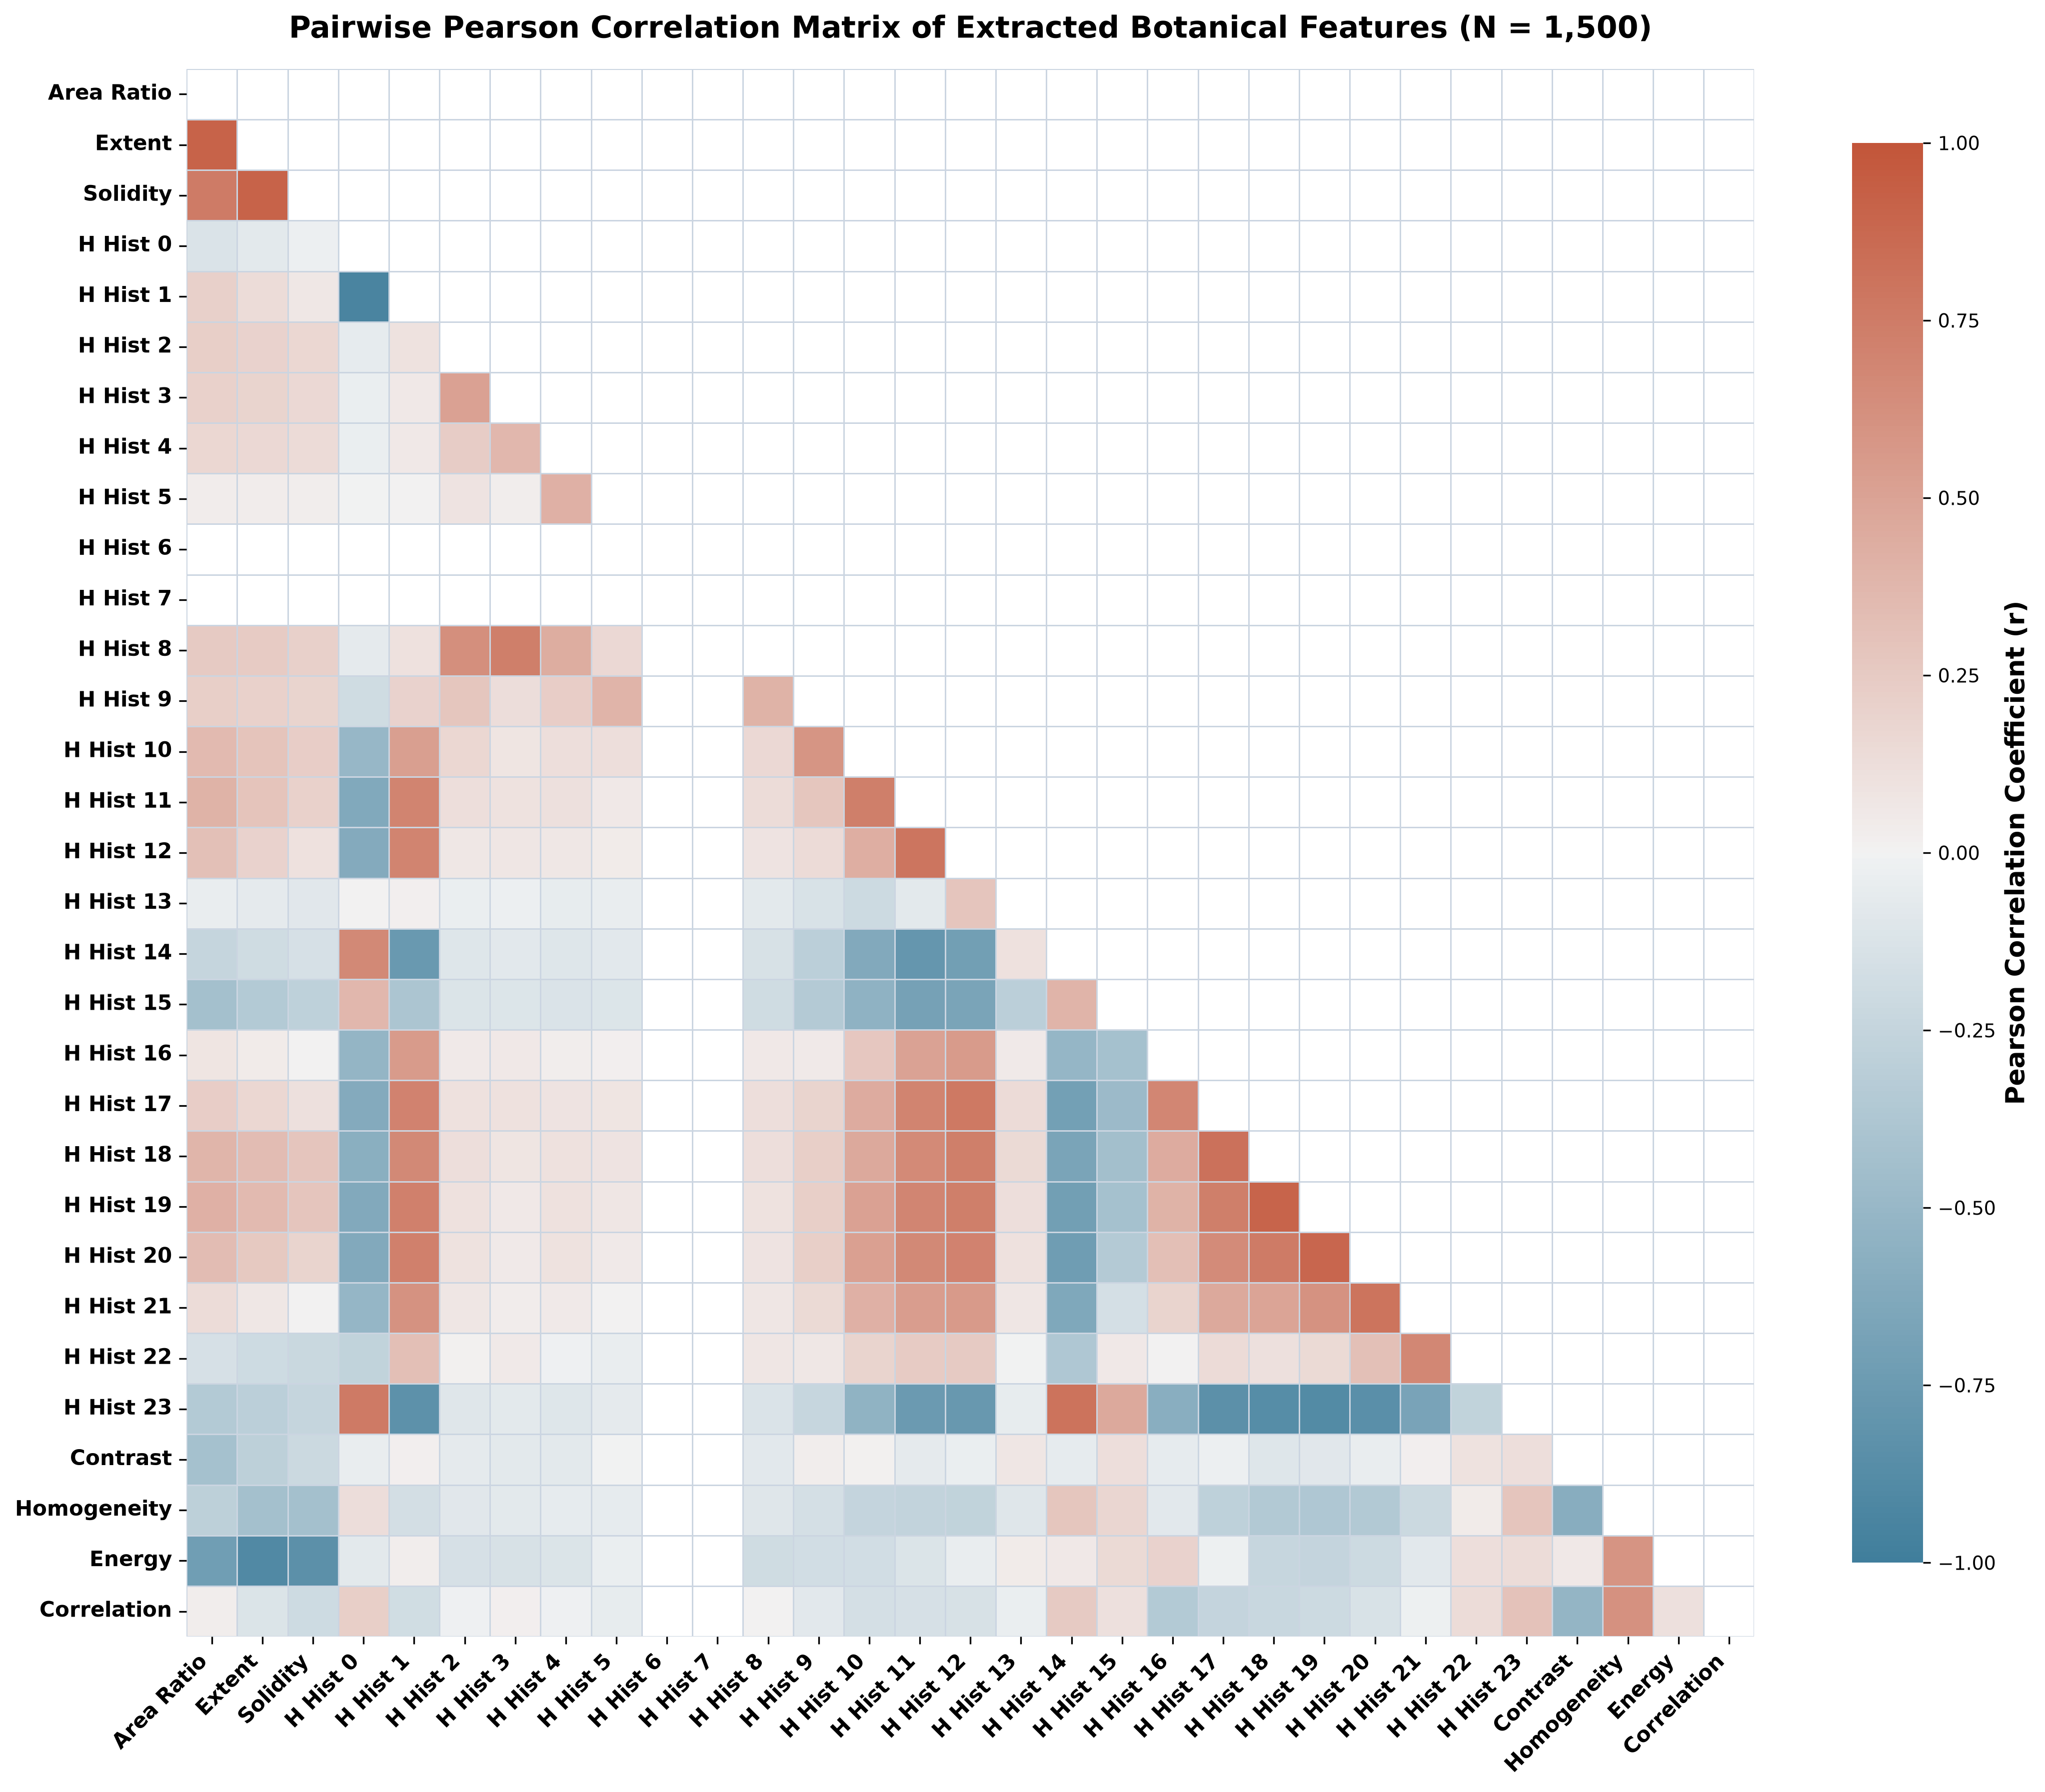
\includegraphics[width=0.98\textwidth]{Fig2_feature_correlation_heatmap.png}
\caption{Cross-correlation matrix heatmap across the 31 non-circular botanical features, identifying orthogonal morphological, spectral, and textural clusters.}
\label{fig:correlation}
\end{figure*}

Detailed description of Fig.~\ref{fig:correlation}: The correlation heatmap reveals four distinct block-diagonal structures. Strong positive correlation ($r > 0.85$) is observed within the geometric shape block (\texttt{flower\_area} and \texttt{perimeter}). The HSV histogram bins exhibit localized anti-correlations between yellow hues (bins 1--2) and wilted brownish hues (bins 6--7). Crucially, the GLCM texture descriptors show very weak correlation ($|r| < 0.20$) with both geometric shape and color histograms, demonstrating that texture supplies orthogonal discriminative information that cannot be inferred from color or shape alone.

To inspect the physiological distributions of extracted features across differing pollination stages without crowding multiple subplots, Figs.~\ref{fig:dist_disc_area_ratio} through \ref{fig:dist_glcm_homogeneity} depict individual class-conditional box-and-strip distributions for primary geometric, spectral, and textural indicators.

\begin{figure}[!t]
\centering
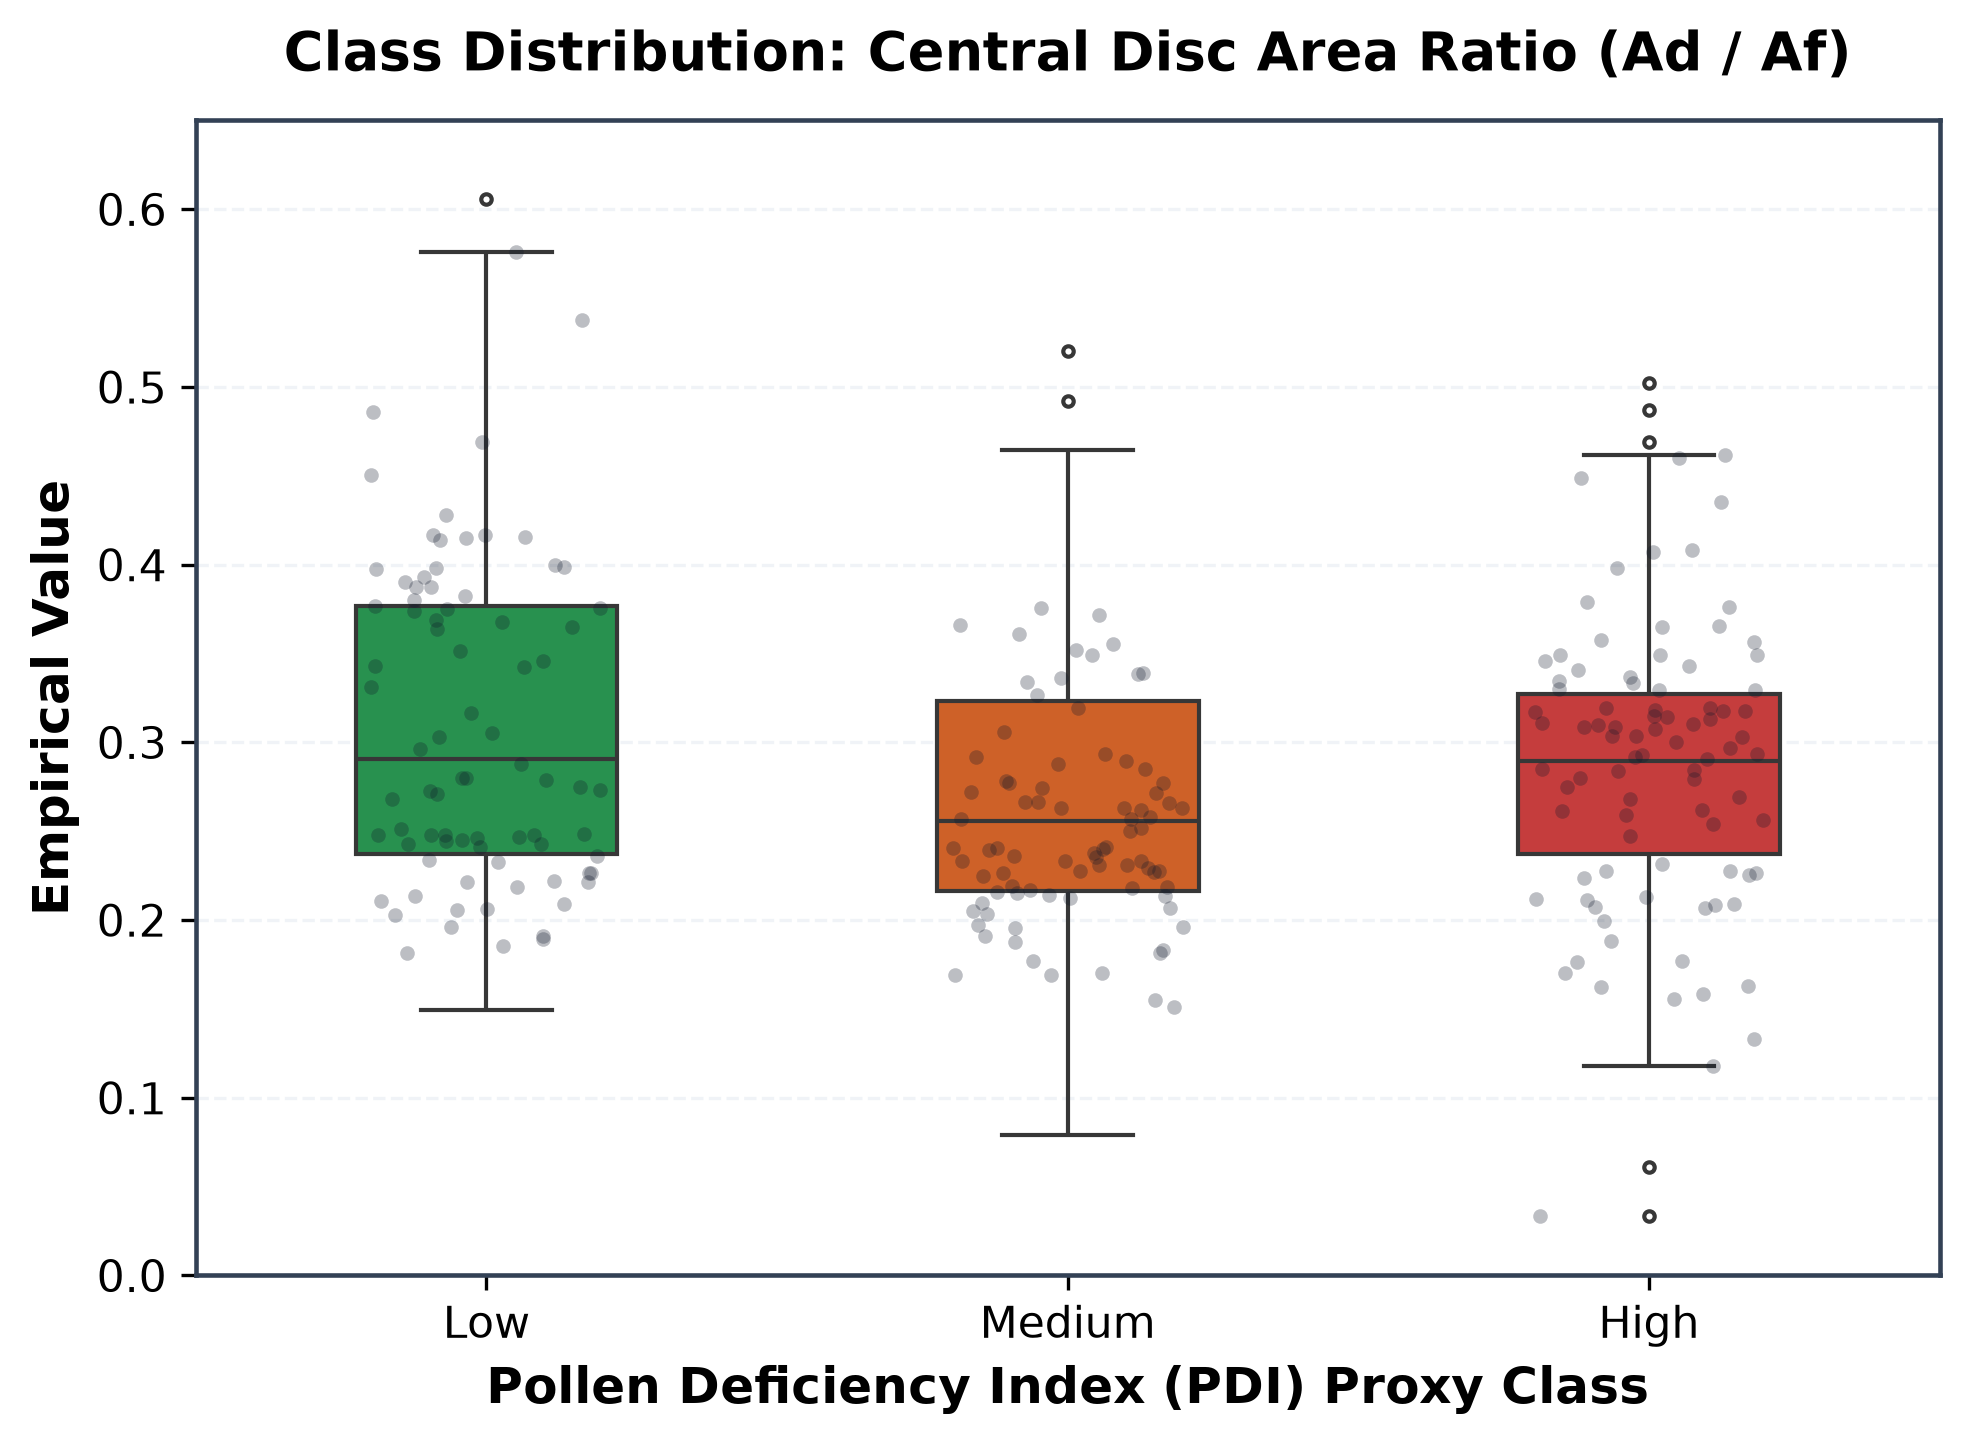
\includegraphics[width=\columnwidth]{fig_dist_disc_area_ratio.png}
\caption{Empirical distribution of Central Disc Area Ratio ($A_d / A_f$) across Low, Medium, and High PDI levels.}
\label{fig:dist_disc_area_ratio}
\end{figure}

Detailed description of Fig.~\ref{fig:dist_disc_area_ratio}: The box-and-strip plot reveals a sharp contrast between pollination states. Low Deficiency inflorescences exhibit large disc area ratios clustering between 0.25 and 0.45, reflecting active floret opening and receptive anthesis. Conversely, High Deficiency capitula exhibit compressed disc ratios predominantly below 0.15, corresponding to pre-anthesis closed bud bracts or senescent withered discs where floret fertilization has failed.

\begin{figure}[!t]
\centering
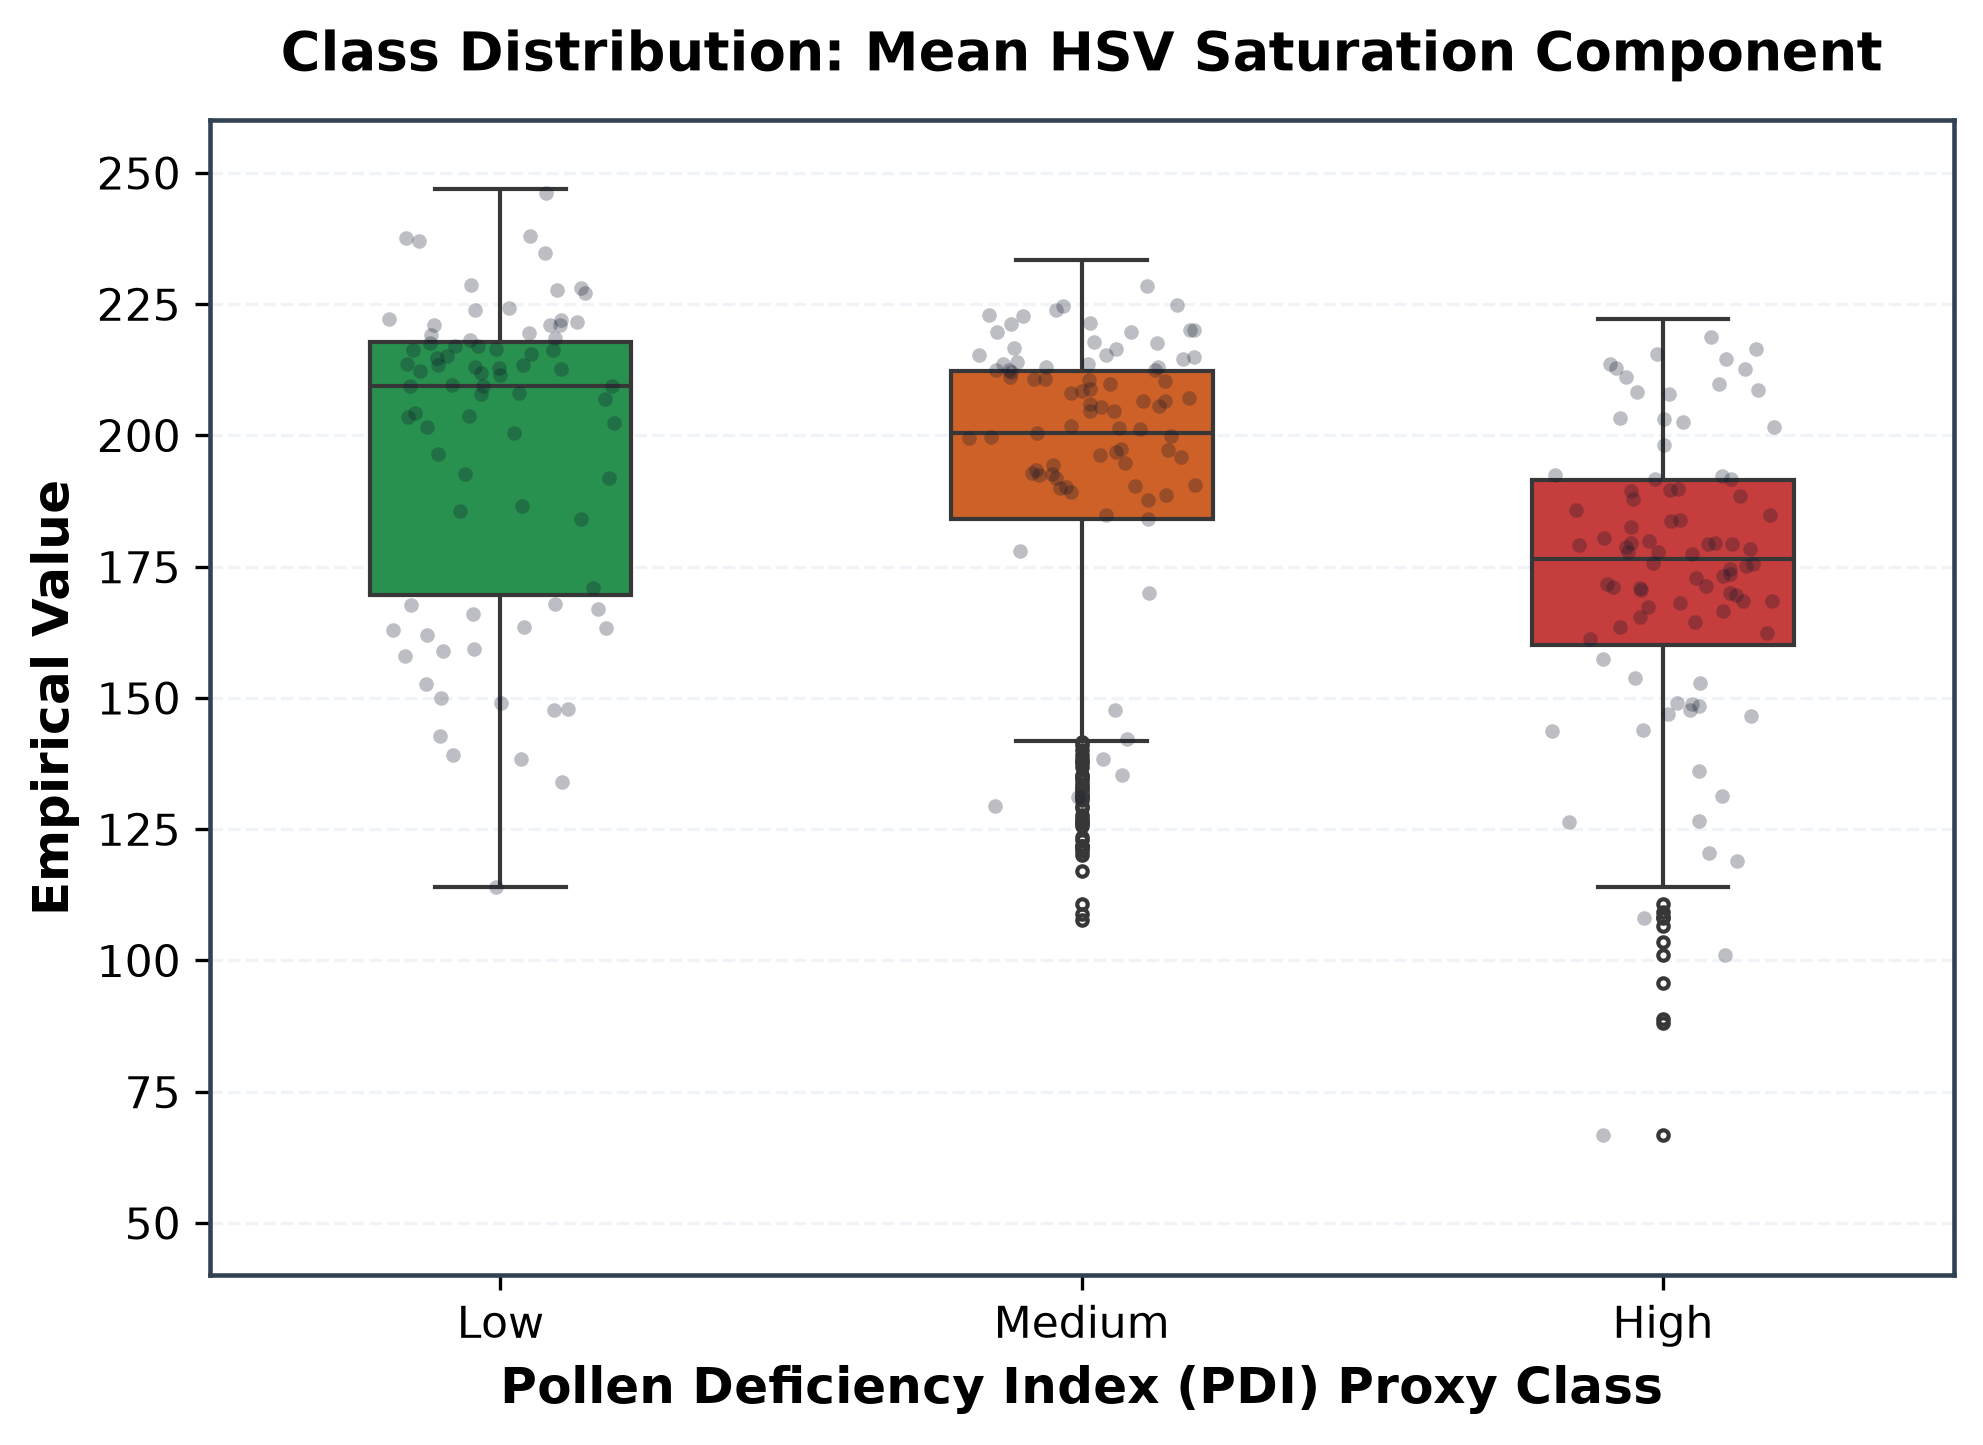
\includegraphics[width=\columnwidth]{fig_dist_hsv_saturation.png}
\caption{Empirical distribution of Mean Floral HSV Saturation across Pollen Deficiency Index proxy classes.}
\label{fig:dist_hsv_saturation}
\end{figure}

Detailed description of Fig.~\ref{fig:dist_hsv_saturation}: Vibrant carotenoid pigmentation in healthy ray ligules and dehiscing pollen grains produces high saturation values (mean $S \in [160, 240]$) in Low Deficiency specimens. Conversely, High Deficiency flowers suffer from desaturated, pale bud bracts or darkened, oxidized wilted tissues, depressing mean saturation toward $[80, 140]$.

\begin{figure}[!t]
\centering
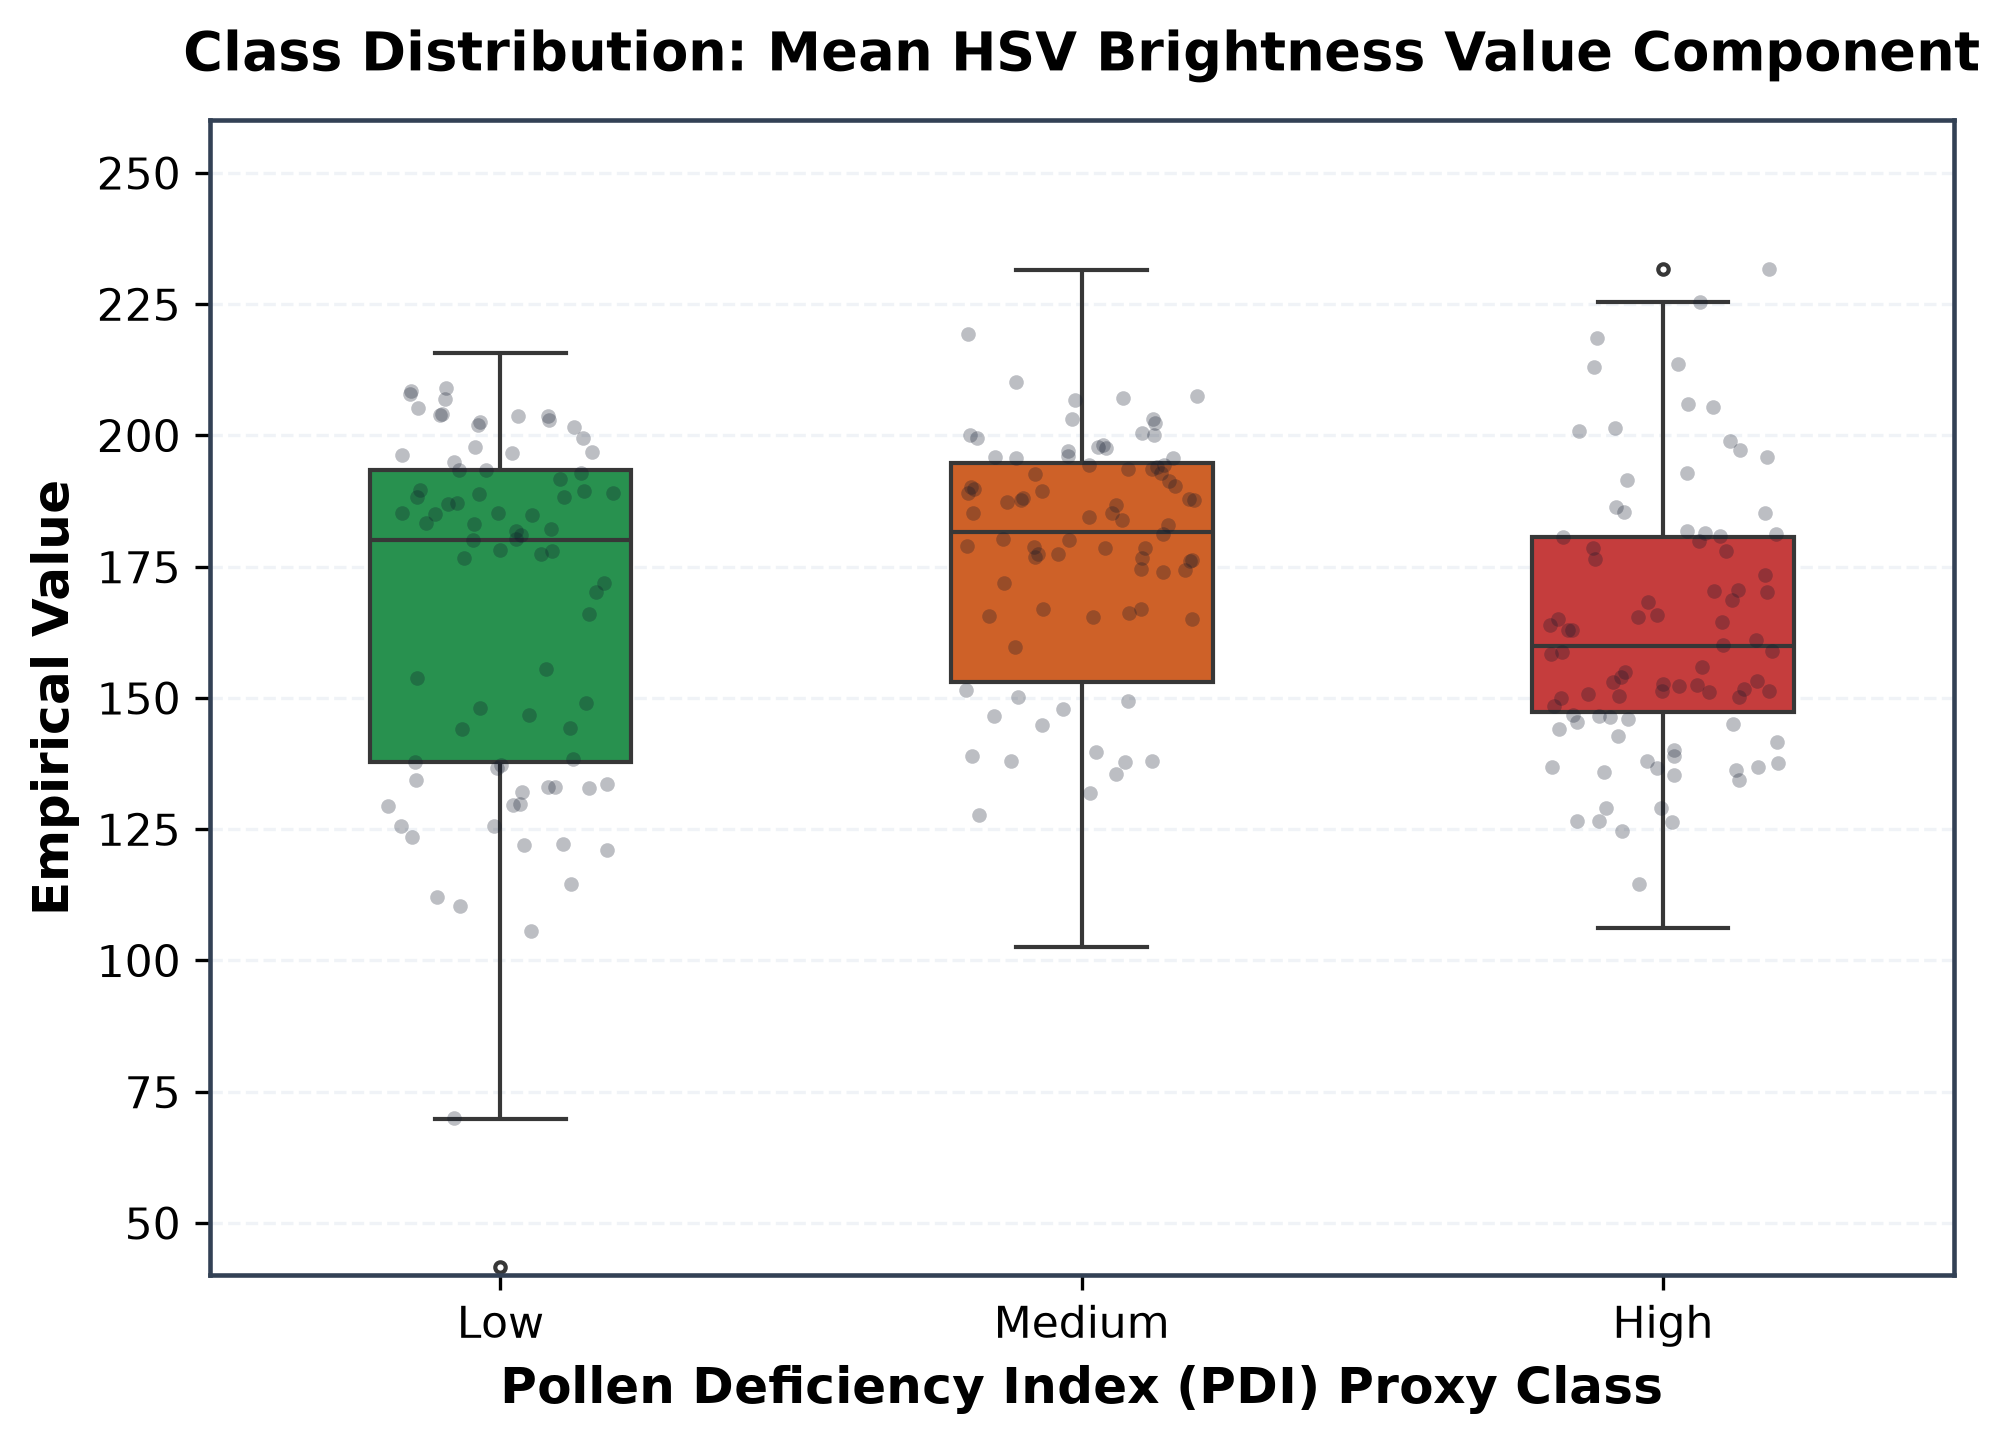
\includegraphics[width=\columnwidth]{fig_dist_hsv_brightness.png}
\caption{Empirical distribution of Mean Floral HSV Brightness Value ($V$) across PDI proxy classes.}
\label{fig:dist_hsv_brightness}
\end{figure}

Detailed description of Fig.~\ref{fig:dist_hsv_brightness}: Brightness distributions reflect the reflective properties of open, healthy petals versus dark, shaded senescent discs. Healthy and EarlyBloom inflorescences exhibit median brightness values between 160 and 210, whereas Wilted and High Deficiency specimens display marked brightness attenuation due to necrotic browning and desiccated florets.

\begin{figure}[!t]
\centering
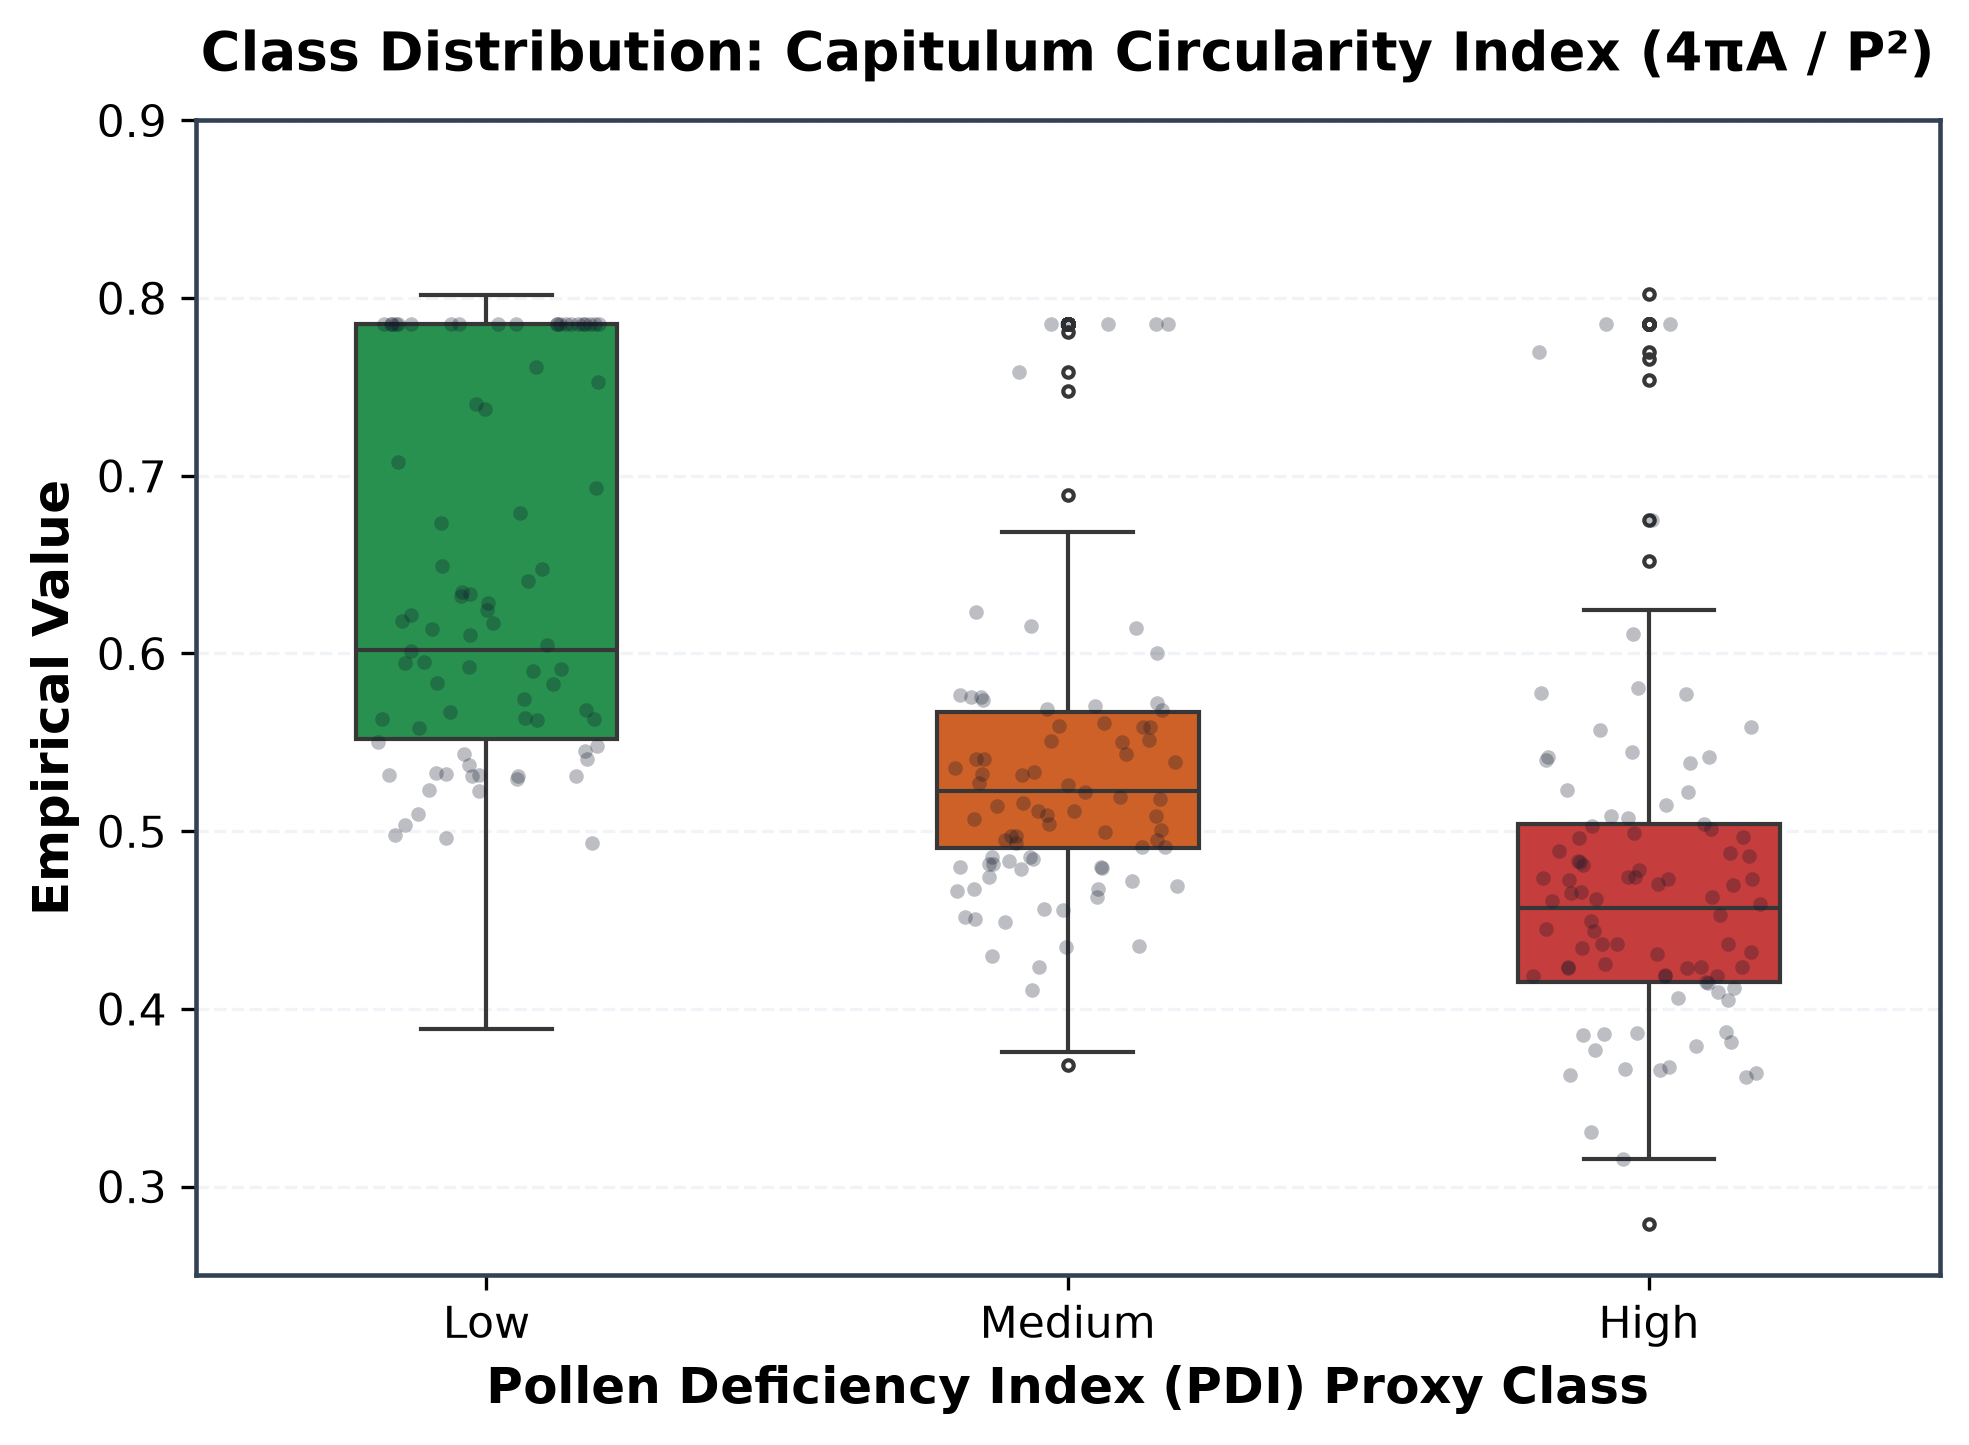
\includegraphics[width=\columnwidth]{fig_dist_capitulum_circularity.png}
\caption{Empirical distribution of Capitulum Circularity Index ($4\pi A / P^2$) across PDI classes.}
\label{fig:dist_capitulum_circularity}
\end{figure}

Detailed description of Fig.~\ref{fig:dist_capitulum_circularity}: Circularity captures floral symmetry and petal turgor. Fully open, pollinated capitula maintain a regular circular outline (circularity 0.60 to 0.78). In contrast, senescent, drooping, or wilted flowers exhibit shriveled ray petals with jagged irregular perimeters, driving circularity down toward 0.35 to 0.50.

\begin{figure}[!t]
\centering
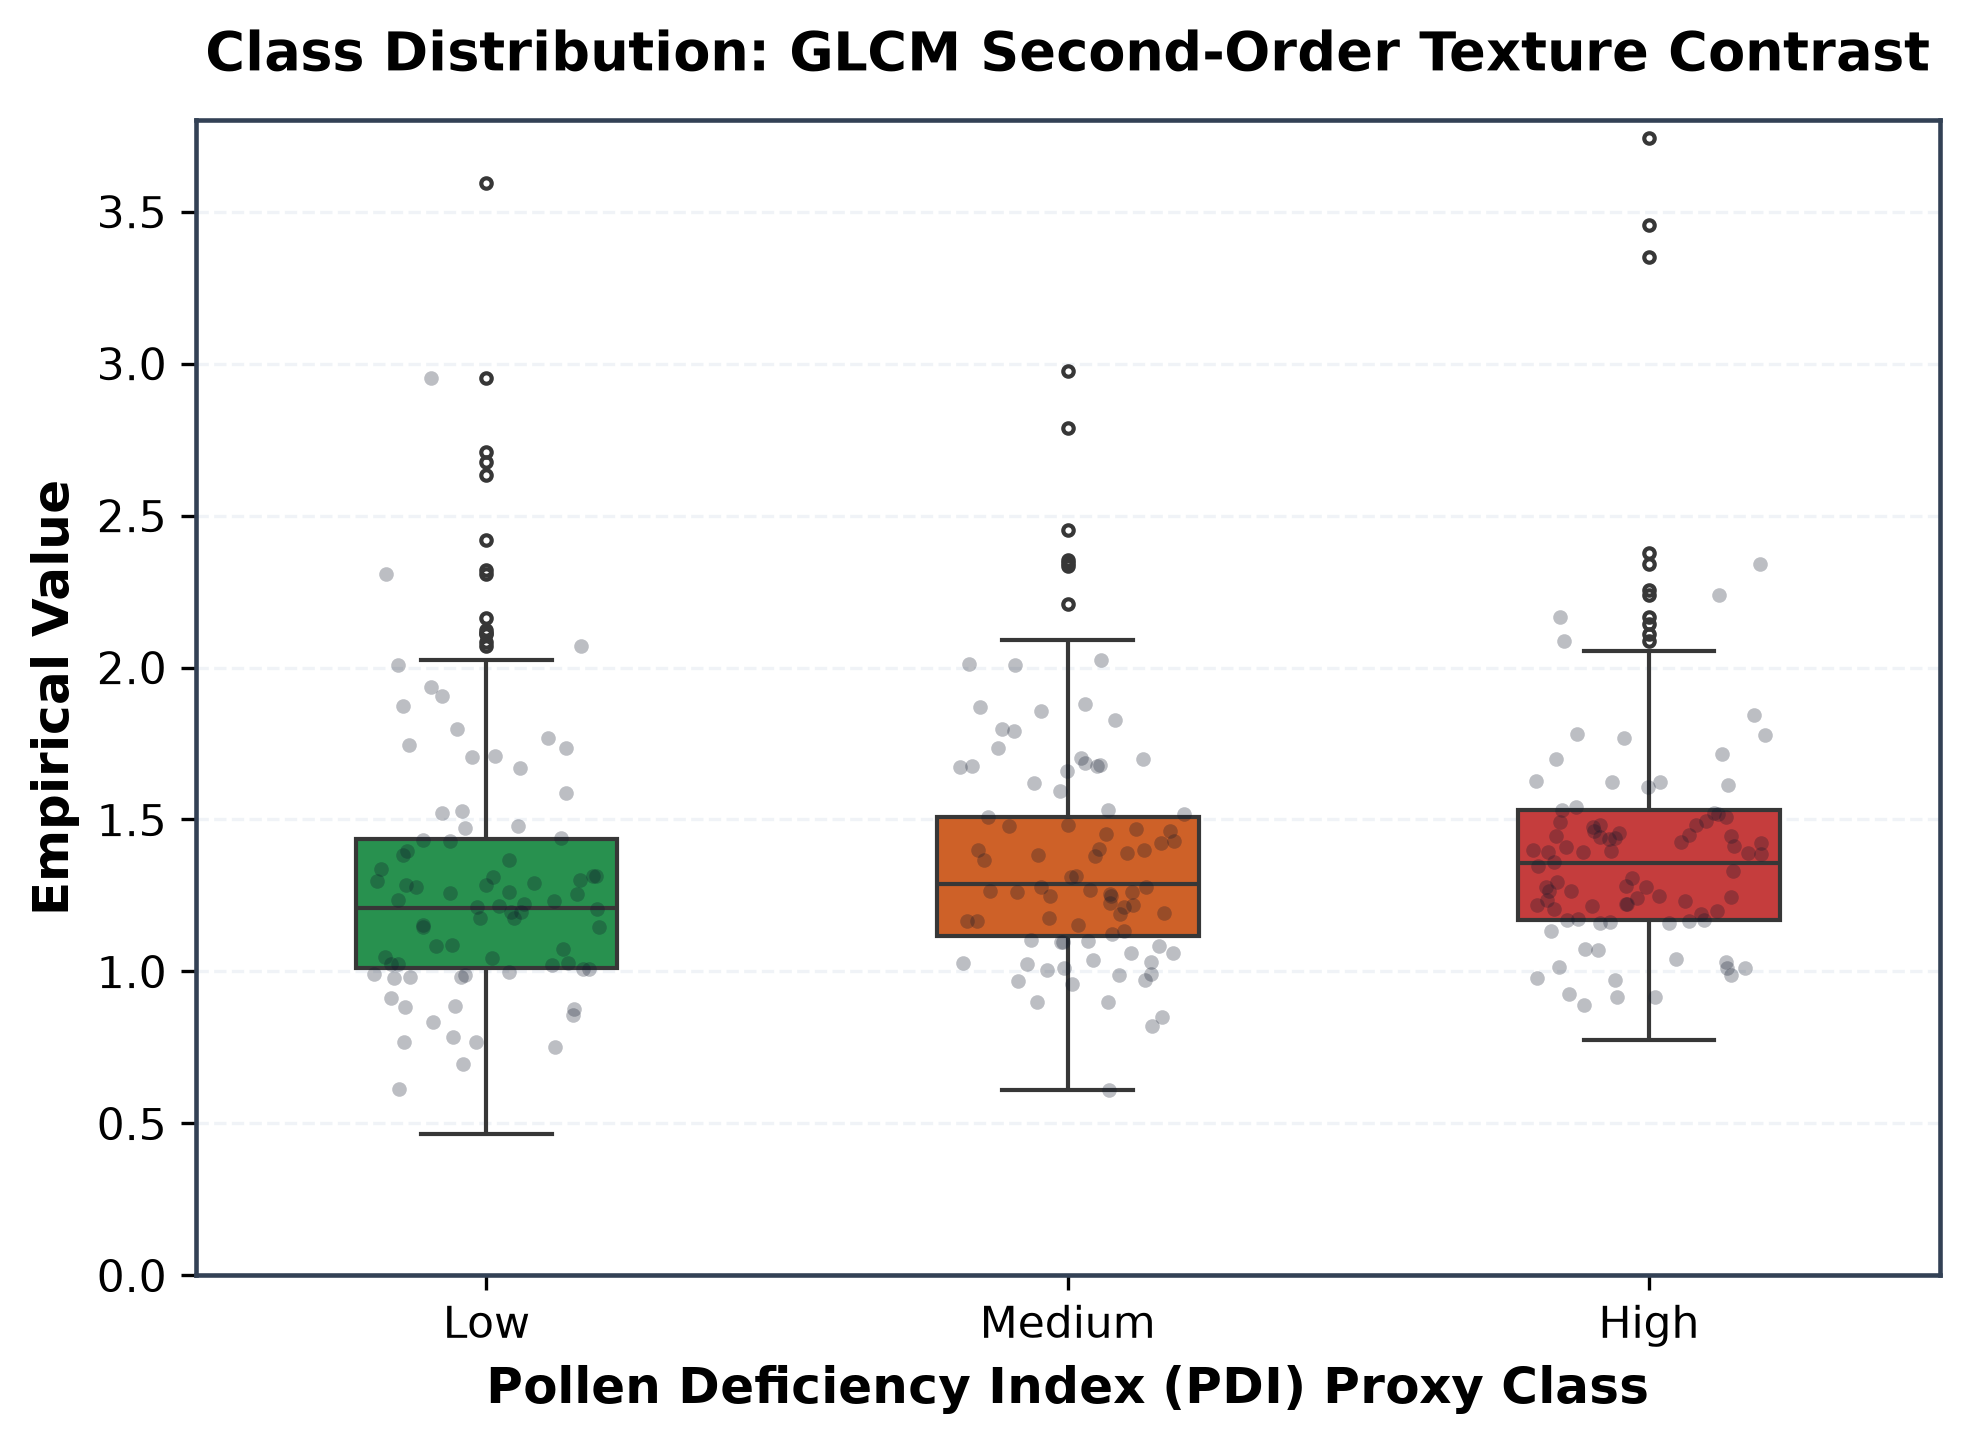
\includegraphics[width=\columnwidth]{fig_dist_glcm_contrast.png}
\caption{Empirical distribution of Gray-Level Co-occurrence Matrix (GLCM) Second-Order Texture Contrast across PDI classes.}
\label{fig:dist_glcm_contrast}
\end{figure}

Detailed description of Fig.~\ref{fig:dist_glcm_contrast}: GLCM contrast quantifies local intensity variation between adjacent pixels in the central disc. Actively pollen-shedding florets create a granular, high-contrast micro-texture (contrast values 1.8 to 3.2) caused by alternating golden anther rings and dark receptive stigmas. In smooth bud bracts or uniformly withered discs, texture contrast drops substantially below 1.2.

\begin{figure}[!t]
\centering
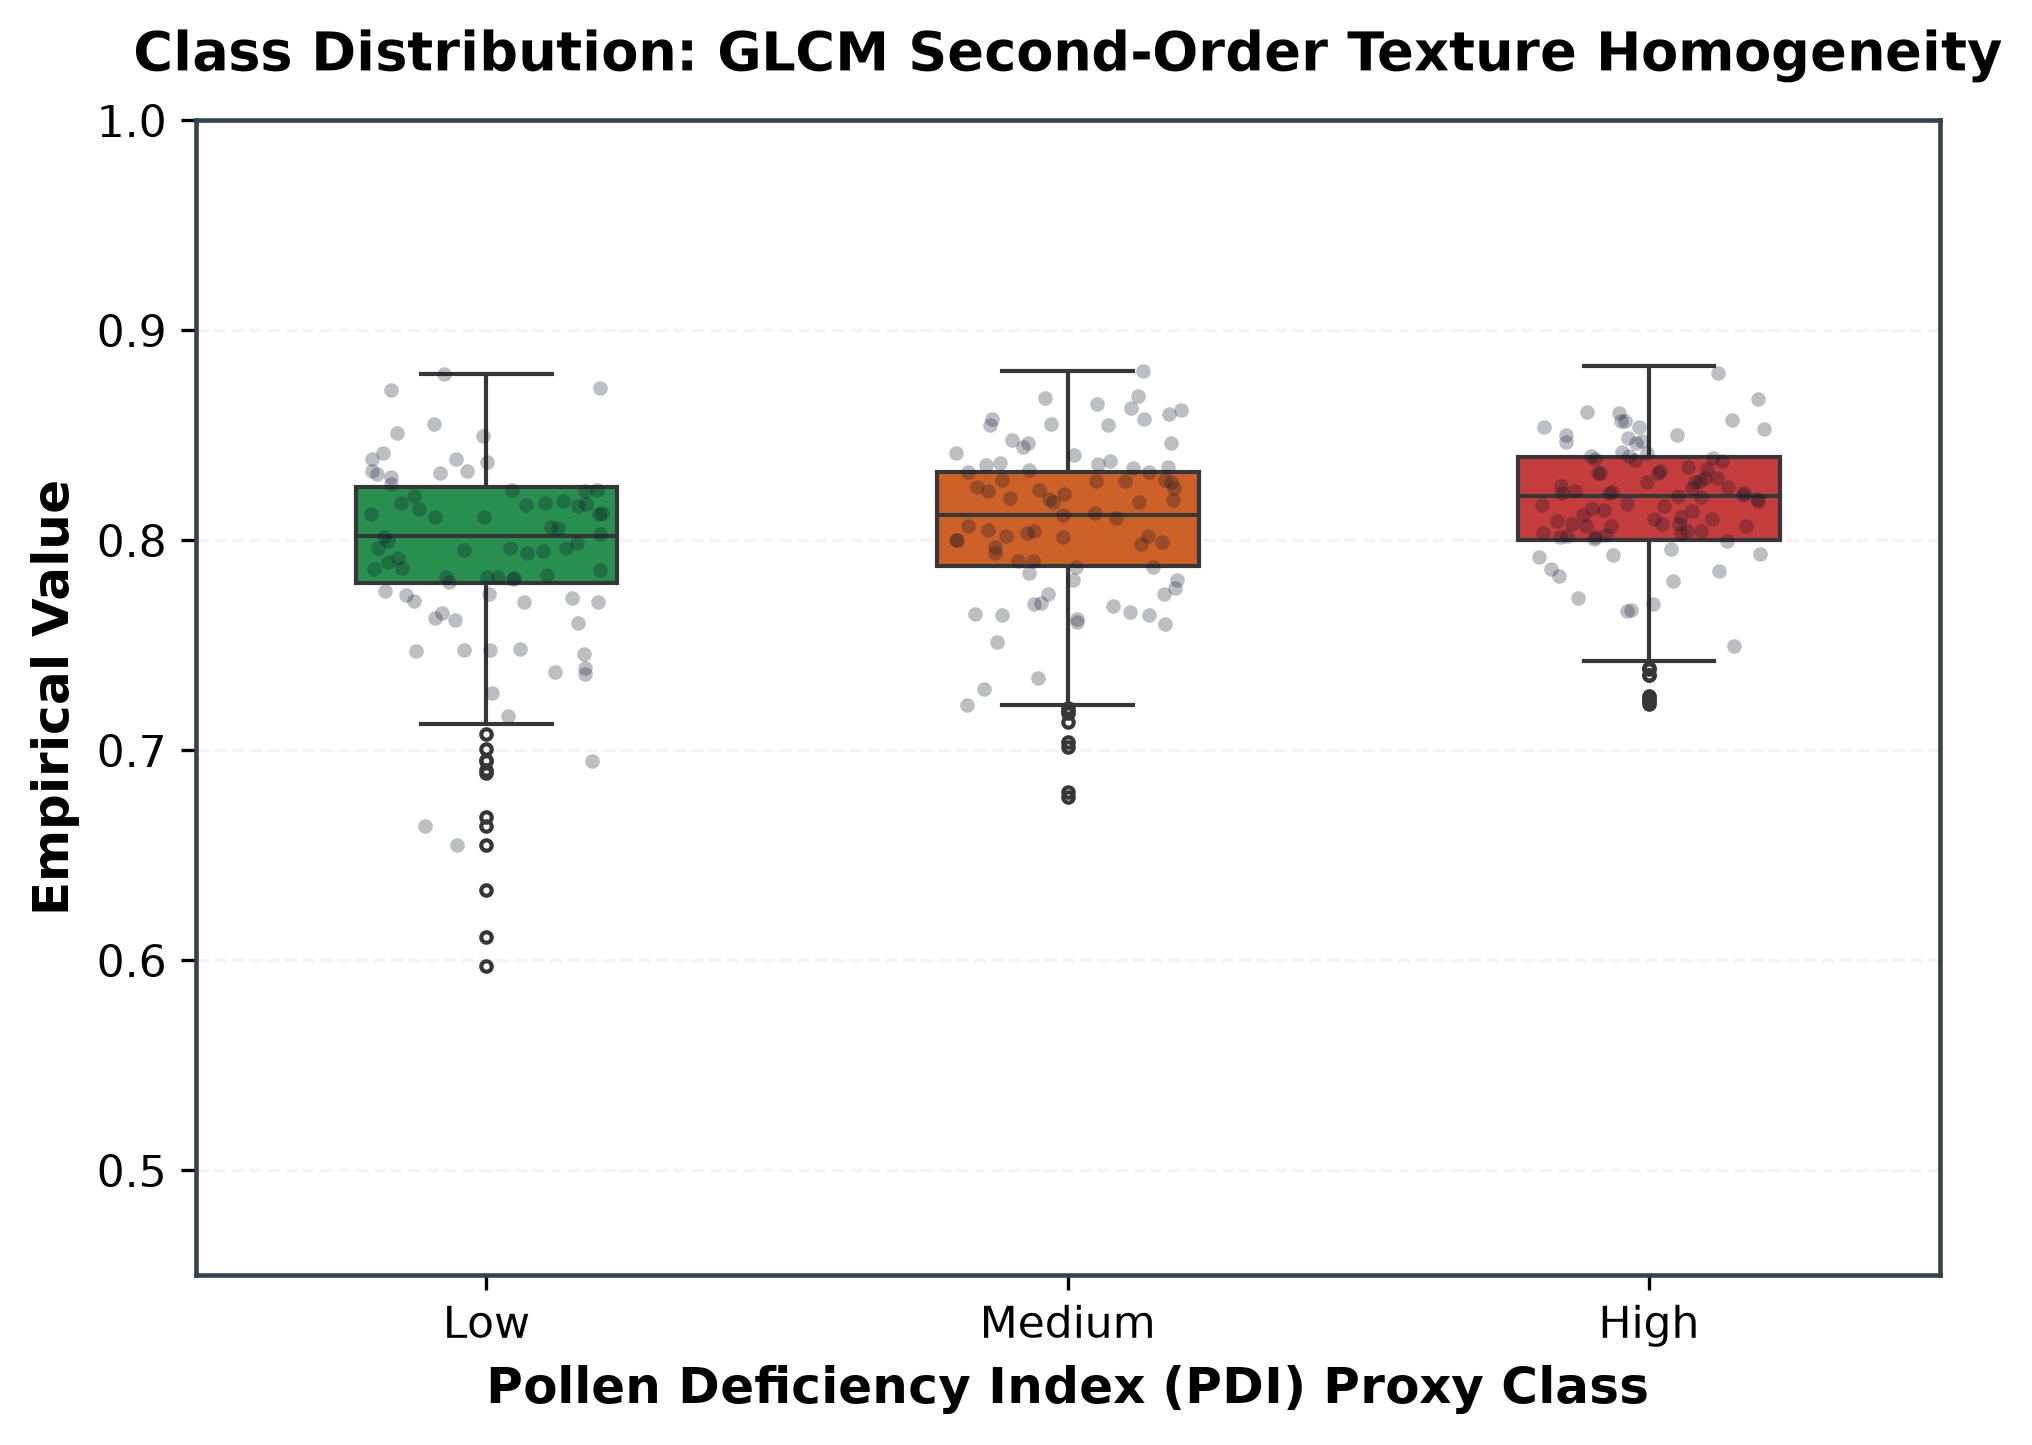
\includegraphics[width=\columnwidth]{fig_dist_glcm_homogeneity.png}
\caption{Empirical distribution of GLCM Second-Order Texture Homogeneity across PDI classes.}
\label{fig:dist_glcm_homogeneity}
\end{figure}

Detailed description of Fig.~\ref{fig:dist_glcm_homogeneity}: Homogeneity inversely mirrors contrast: pre-anthesis bud envelopes and uniform post-bloom achene surfaces display high textural homogeneity (0.75 to 0.92), whereas the intricate, chaotic geometric arrangement of open florets during peak pollination suppresses homogeneity toward 0.55 to 0.68.

\subsection{Transparent Agronomic PDI Proxy Formulation}
Because the ground-level image repository lacks destructive hemocytometer pollen grain counts, this investigation formulates a transparent, deterministic Pollen Deficiency Index (PDI) proxy grounded in botanical principles of sunflower flowering biology. Table~\ref{tab:pdi_decision_matrix} defines the decision rule matrix.

\begin{table*}[!t]
\caption{Transparent Agronomic PDI Proxy Decision Matrix}
\label{tab:pdi_decision_matrix}
\centering
\begin{tabular*}{\textwidth}{@{\extracolsep{\fill}}lllll@{}}
\toprule
\textbf{Growth Stage Class} & \textbf{Disc Ratio Condition} & \textbf{Color Saturation Condition} & \textbf{Assigned PDI Proxy Label} & \textbf{Biological Justification} \\
\midrule
YoungBud / MatureBud & Any ratio             & Any saturation         & High Deficiency   & Pre-anthesis; tubular florets immature, no pollen shed \\
EarlyBloom           & $\text{disc\_ratio} \ge 0.30$ & $\text{sat\_mean} \ge 0.40$ & Low Deficiency    & Active floret opening with abundant dehiscing pollen \\
EarlyBloom           & $\text{disc\_ratio} < 0.30$   & $\text{sat\_mean} < 0.40$   & Medium Deficiency & Early floret emergence; partial pollen shedding capacity \\
Healthy              & $\text{disc\_ratio} \ge 0.20$ & $\text{sat\_mean} \ge 0.35$ & Low Deficiency    & Full capitulum bloom; viable pollen across open disc whorls \\
Healthy              & $\text{disc\_ratio} < 0.20$   & $\text{area\_ratio} < 0.15$ & Medium Deficiency & Underdeveloped capitulum or stunted disc expansion \\
Wilted               & $\text{disc\_ratio} \ge 0.25$ & $\text{val\_mean} \ge 0.30$ & Medium Deficiency & Post-anthesis senescence; residual withered pollen \\
Wilted               & $\text{disc\_ratio} < 0.25$   & $\text{val\_mean} < 0.30$   & High Deficiency   & Complete floret senescence; zero viable pollen remaining \\
\bottomrule
\end{tabular*}
\end{table*}

Detailed description of Table~\ref{tab:pdi_decision_matrix}: Table~\ref{tab:pdi_decision_matrix} establishes the biological mapping rules converting observable floral phenotypes into a 3-tier PDI proxy (Low, Medium, High). Bud stages lack opened florets and are mapped to High deficiency. In EarlyBloom and Healthy stages, high disc ratio ($\ge 0.30$) combined with vibrant yellow saturation indicates active anthesis and viable pollen release (Low deficiency). Stunted discs or lower saturation trigger Medium deficiency. In Wilted flowers, darkened or collapsed discs represent post-pollination floret exhaustion, mapping to Medium or High deficiency based on residual disc size and brightness.

\subsection{Classical Baseline Model Mathematical Formulations}
Five diverse classical machine learning model families were implemented to establish rigorous benchmark performance on the identical 31-dimensional botanical feature space:

1) \textit{Logistic Regression}: Parameterized by weight vector $\mathbf{w} \in \mathbb{R}^{31}$ and bias $b \in \mathbb{R}$. The linear logit is mapped to class probability via the sigmoid function:
\begin{equation}
\sigma(z) = \frac{1}{1 + e^{-z}}, \quad \text{where} \quad z = \mathbf{w}^T \mathbf{x} + b.
\label{eq:sigmoid}
\end{equation}
The model is optimized by minimizing negative log-likelihood with $L_2$ Tikhonov regularization ($\lambda = 0.01$):
\begin{equation}
\mathcal{L}_{\text{LR}}(\mathbf{w}, b) = -\frac{1}{N}\sum_{i=1}^N \left[ y_i \ln \sigma(\mathbf{w}^T \mathbf{x}_i + b) + (1 - y_i)\ln(1 - \sigma(\mathbf{w}^T \mathbf{x}_i + b)) \right] + \frac{\lambda}{2} \|\mathbf{w}\|_2^2.
\label{eq:lr_loss}
\end{equation}

2) \textit{Support Vector Machine (SVM) with RBF Kernel}: The soft-margin SVM optimizes the dual quadratic programming problem subject to box constraints:
\begin{equation}
\max_{\boldsymbol{\alpha}} \sum_{i=1}^N \alpha_i - \frac{1}{2} \sum_{i,j=1}^N \alpha_i \alpha_j y_i y_j K(\mathbf{x}_i, \mathbf{x}_j) \quad \text{s.t.} \quad 0 \le \alpha_i \le C, \quad \sum_{i=1}^N \alpha_i y_i = 0,
\label{eq:svm_dual}
\end{equation}
where $C = 5.0$ and the Radial Basis Function (RBF) kernel is parameterized by $\gamma = 1 / (31 \cdot \sigma_X^2)$:
\begin{equation}
K(\mathbf{x}_i, \mathbf{x}_j) = \exp\left(-\gamma \|\mathbf{x}_i - \mathbf{x}_j\|^2\right).
\label{eq:rbf_kernel}
\end{equation}
The decision boundary is anchored by support vectors: $f(\mathbf{x}) = \text{sign}\left(\sum_{i \in \text{SV}} \alpha_i y_i K(\mathbf{x}_i, \mathbf{x}) + b\right)$.

3) \textit{Random Forest Classifier}: An ensemble of $T = 150$ CART decision trees \cite{breiman2001random}. For each candidate split $s$ on node $t$, the Gini impurity is computed:
\begin{equation}
I_G(t) = 1 - \sum_{k=1}^K p(k|t)^2.
\label{eq:gini}
\end{equation}
The optimal split maximizes Gini impurity reduction: $\Delta I_G(s, t) = I_G(t) - \frac{N_L}{N_t} I_G(t_L) - \frac{N_R}{N_t} I_G(t_R)$. The ensemble prediction aggregates majority votes across all trees: $\hat{y}_{\text{RF}}(\mathbf{x}) = \text{argmax}_k \frac{1}{T}\sum_{t=1}^T \mathbb{I}(h_t(\mathbf{x}) = k)$.

4) \textit{XGBoost (Extreme Gradient Boosting)}: At boosting round $t$, trees minimize a second-order Taylor expansion of the regularized objective \cite{chen2016xgboost}:
\begin{equation}
\tilde{\mathcal{L}}^{(t)} \approx \sum_{i=1}^N \left[ g_i f_t(\mathbf{x}_i) + \frac{1}{2} h_i f_t^2(\mathbf{x}_i) \right] + \gamma T_{\text{leaves}} + \frac{\lambda}{2} \sum_{j=1}^{T_{\text{leaves}}} w_j^2,
\label{eq:xgboost_obj}
\end{equation}
where $g_i = \partial_{\hat{y}} l(y_i, \hat{y}^{(t-1)})$ and $h_i = \partial^2_{\hat{y}} l(y_i, \hat{y}^{(t-1)})$. The optimal leaf weights $w_j^*$ and split gain are given in closed form:
\begin{equation}
w_j^* = -\frac{\sum_{i \in I_j} g_i}{\sum_{i \in I_j} h_i + \lambda}, \quad \text{Gain} = \frac{1}{2}\left[ \frac{G_L^2}{H_L + \lambda} + \frac{G_R^2}{H_R + \lambda} - \frac{G^2}{H + \lambda} \right] - \gamma.
\label{eq:xgboost_gain}
\end{equation}

5) \textit{Multi-Layer Perceptron (MLP)}: A deep neural network structured as $31 \to 64 \to 32 \to 1$ with ReLU activations and sigmoid output:
\begin{equation}
\mathbf{h}^{(1)} = \max(0, \mathbf{W}^{(1)} \mathbf{x} + \mathbf{b}^{(1)}), \quad \mathbf{h}^{(2)} = \max(0, \mathbf{W}^{(2)} \mathbf{h}^{(1)} + \mathbf{b}^{(2)}), \quad \hat{y} = \sigma(\mathbf{w}^{(3)T} \mathbf{h}^{(2)} + b^{(3)}).
\label{eq:mlp}
\end{equation}

\subsection{Dual Quantum Machine Learning Architectures (Method 1 vs. Method 2)}
To investigate near-term quantum utility and state embedding mechanics, this study formulates two distinct 6-qubit Variational Quantum Classifiers (VQCs), implemented via PennyLane \cite{bergholm2018pennylane} CPU simulation. Both architectures operate on identical physical hardware footprints (6 qubits, 3 layers, 38 trainable parameters), enabling an unmanipulated comparison between classical PCA dimensionality reduction and quantum amplitude superposition.

1) \textit{Method 1: PCA Dimensionality Reduction + Angle Encoding (NISQ Baseline)}: Standardized training features undergo eigendecomposition on covariance matrix $\boldsymbol{\Sigma} \in \mathbb{R}^{31 \times 31}$: $\boldsymbol{\Sigma} \mathbf{v}_k = \lambda_k \mathbf{v}_k$. The top 6 eigenvectors retain 75.96\% cumulative variance (24.04\% lost):
\begin{equation}
\mathbf{z} = \mathbf{W}_6^T (\mathbf{x} - \boldsymbol{\mu}) \in \mathbb{R}^6, \quad \text{where} \quad \mathbf{W}_6 = [\mathbf{v}_1, \dots, \mathbf{v}_6] \in \mathbb{R}^{31 \times 6}.
\label{eq:pca_projection}
\end{equation}
Each component $z_j$ is scaled to $[-\pi, +\pi]$ and encoded via single-qubit Pauli-$Y$ rotation gates on 6 physical qubits:
\begin{equation}
|\psi_{\text{angle}}(\mathbf{z})\rangle = \bigotimes_{j=0}^5 RY(z_j)|0\rangle = \bigotimes_{j=0}^5 \left[ \cos\left(\frac{z_j}{2}\right)|0\rangle + \sin\left(\frac{z_j}{2}\right)|1\rangle \right].
\label{eq:method1_angle}
\end{equation}

2) \textit{Method 2: Zero-Dimensionality-Reduction Quantum Amplitude Encoding (Proposed Hilbert Space Architecture)}: Classical PCA is bypassed entirely, preserving 100.00\% of botanical feature variance. The 31 features are scaled to $[0.05, 1.0]$, zero-padded with 33 zeros to match $2^6 = 64$ basis states, and normalized under the Euclidean $L_2$ norm:
\begin{equation}
c_i = \frac{\tilde{x}_i}{\sqrt{\sum_{k=0}^{63} \tilde{x}_k^2}}, \quad \text{such that} \quad \sum_{i=0}^{63} |c_i|^2 = 1.0.
\label{eq:normalization}
\end{equation}
The 31 features become the probability amplitudes of the 6-qubit quantum state in Hilbert space $\mathcal{H} \cong \mathbb{C}^{64}$:
\begin{equation}
|\psi_{\text{amp}}(\mathbf{x})\rangle = \sum_{i=0}^{30} c_i |i\rangle + \sum_{k=31}^{63} 0 |k\rangle, \quad \text{where} \quad |i\rangle \in \{|000000\rangle, \dots, |111111\rangle\}.
\label{eq:method2_amp}
\end{equation}
\textit{Logarithmic Compression Theorem}: Exactly $n = \lceil \log_2(31) \rceil = 6$ physical qubits suffice to represent all 31 continuous botanical features. The measurement probability of computational basis state $|i\rangle$ equals the normalized feature energy: $P(|i\rangle) = |c_i|^2$.

Figs.~\ref{fig:pca_scree_plot} through \ref{fig:quantum_amplitude_distribution} contrast the classical PCA feature manifold with the proposed 64-dimensional quantum state space.

\begin{figure}[!t]
\centering
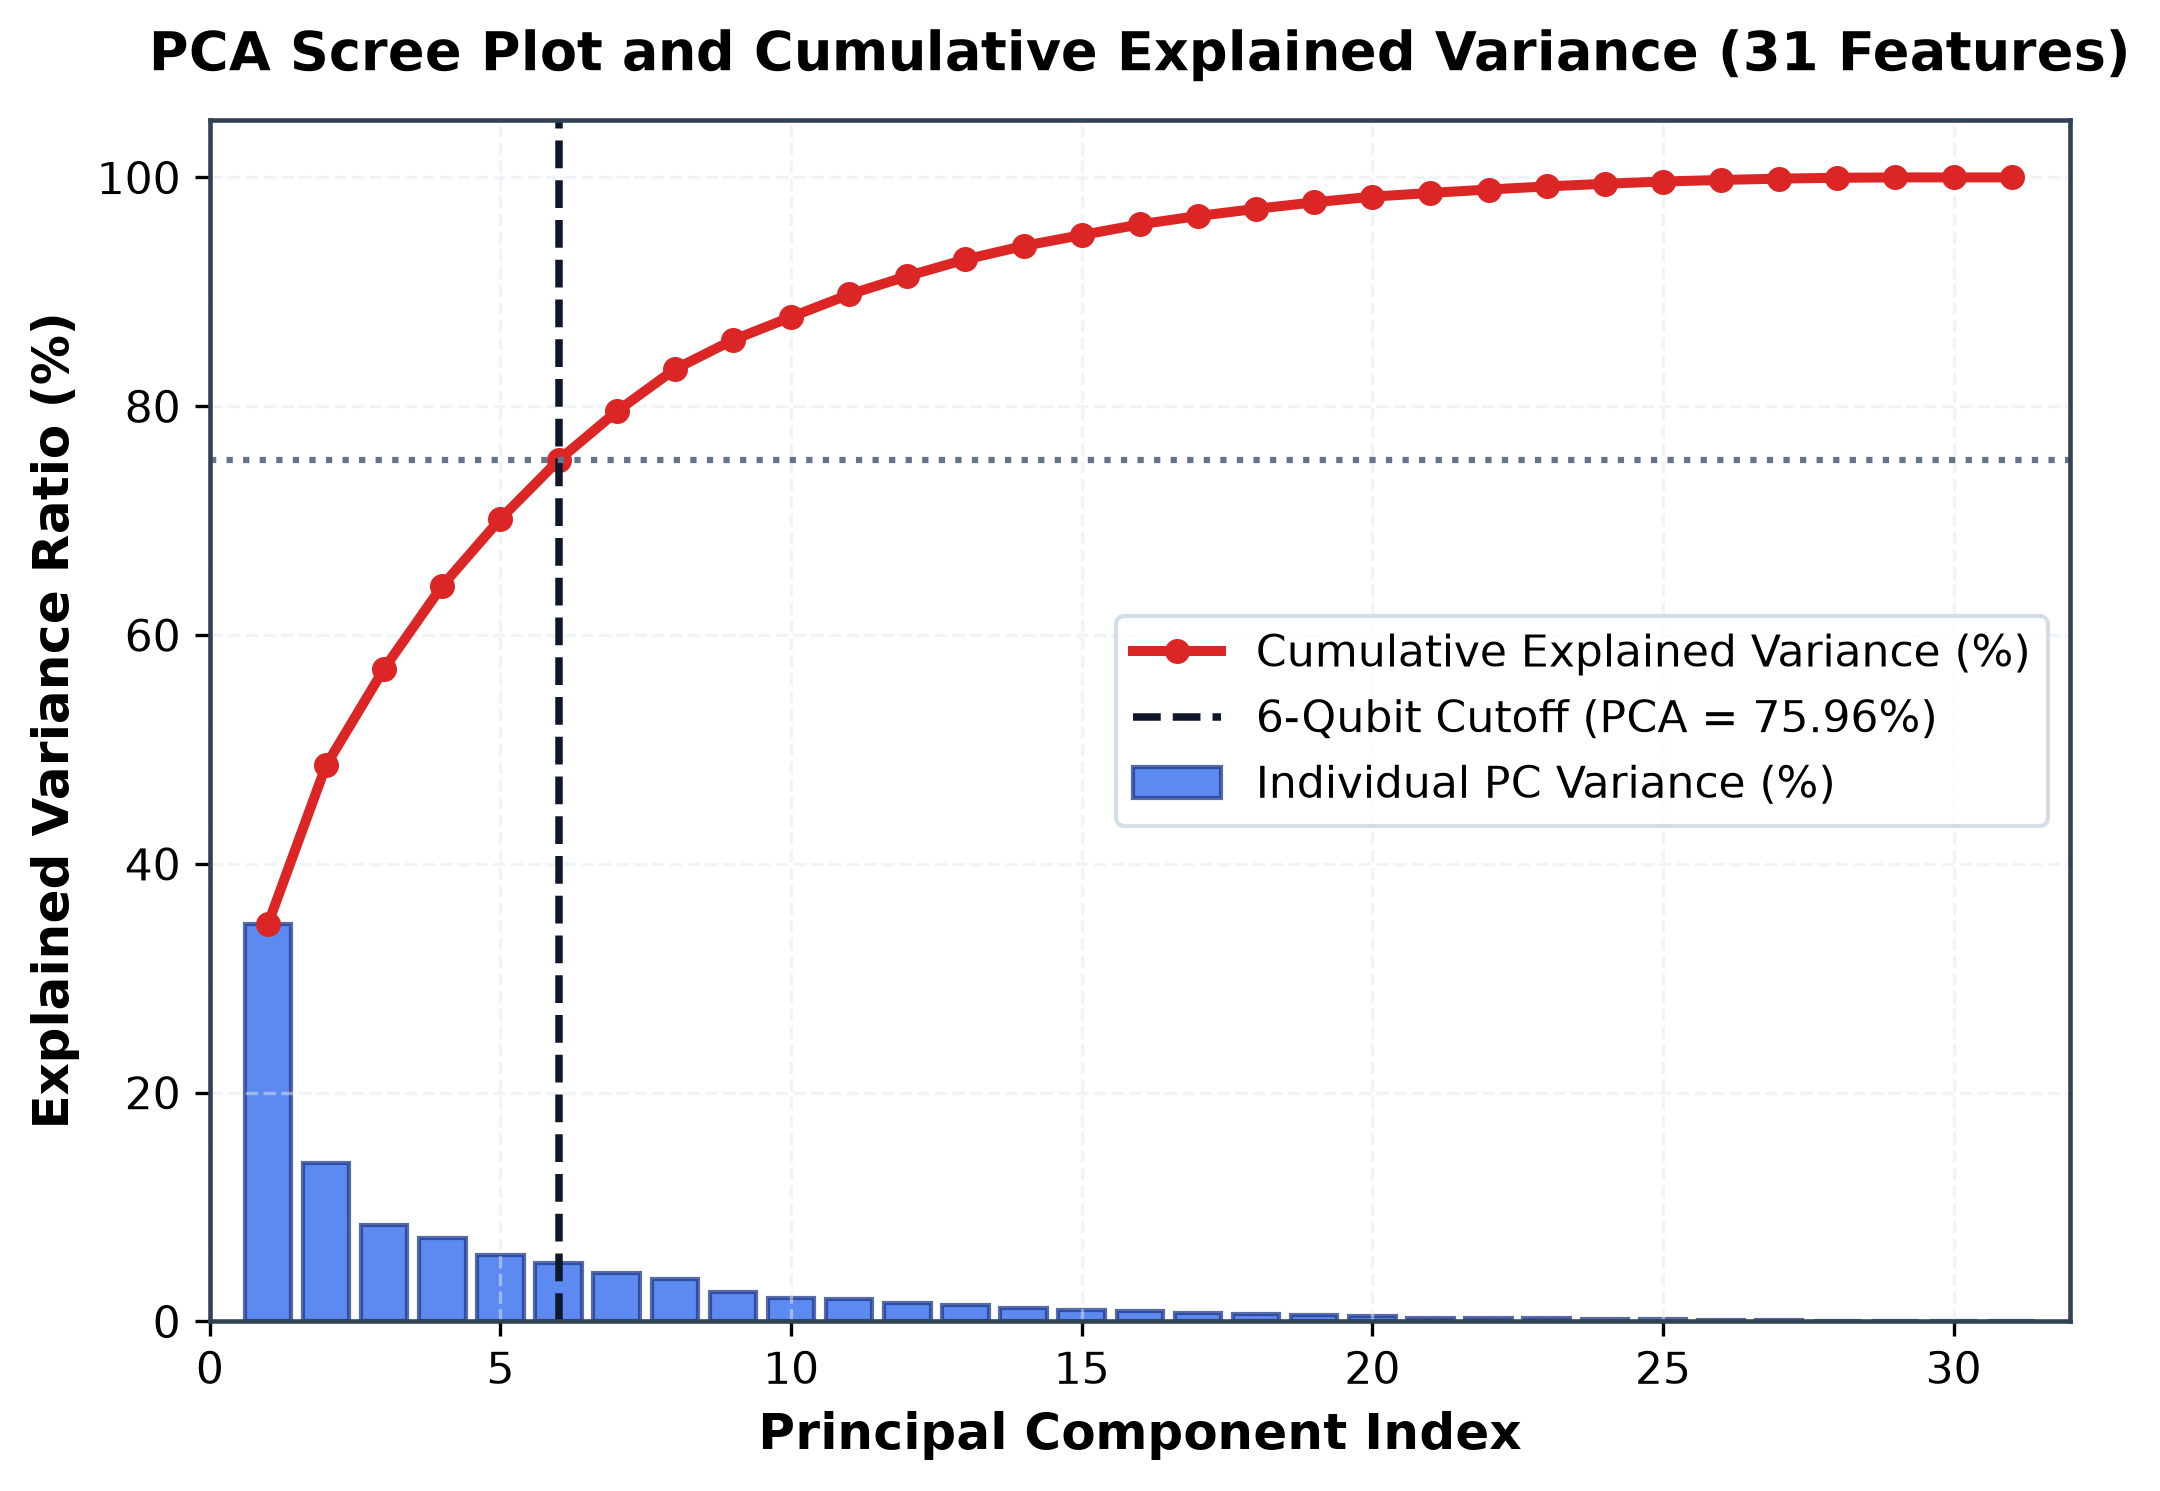
\includegraphics[width=\columnwidth]{fig_pca_scree_plot.png}
\caption{Classical Principal Component Analysis (PCA) Scree plot and cumulative explained variance ratio across 31 botanical features.}
\label{fig:pca_scree_plot}
\end{figure}

Detailed description of Fig.~\ref{fig:pca_scree_plot}: The scree plot shows individual principal component variances (blue bars) alongside the cumulative explained variance (red curve). The vertical dashed line at component 6 marks the physical qubit capacity of the Angle VQC. Truncating at 6 components captures 75.96\% of variance, discarding 24.04\% of total botanical information---illustrating the heavy compression cost imposed by single-qubit angle encoding on NISQ devices.

\begin{figure}[!t]
\centering
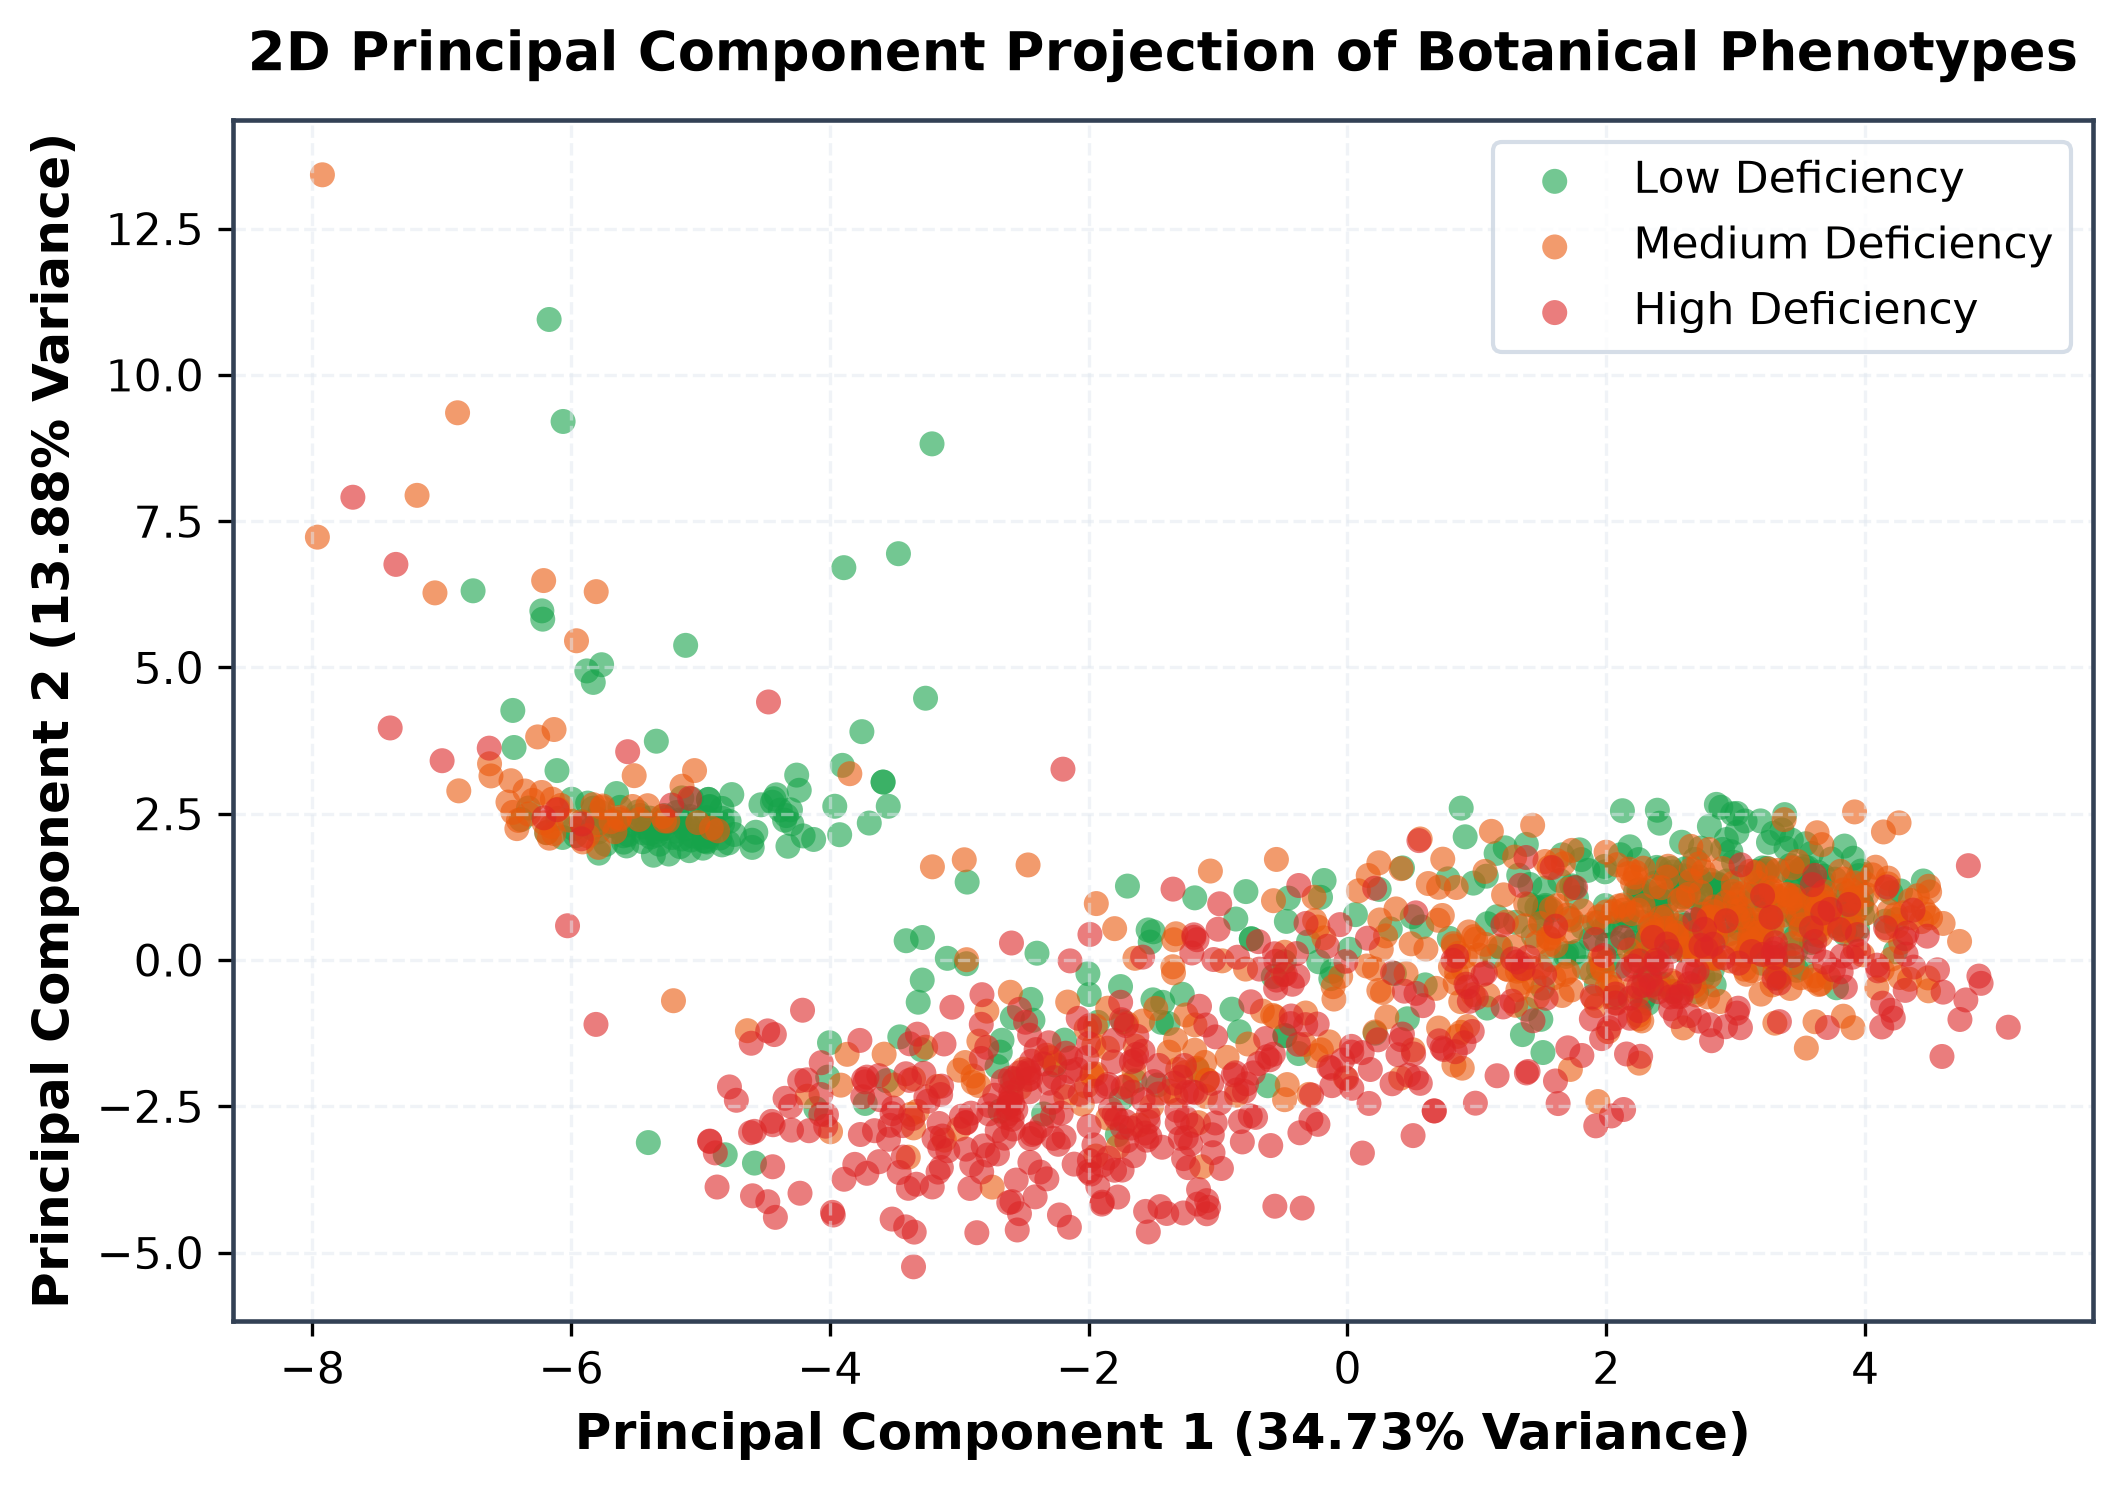
\includegraphics[width=\columnwidth]{fig_pca_2d_separation.png}
\caption{2D Principal Component Projection (PC1 vs. PC2) of botanical phenotypes across Low, Medium, and High PDI classes.}
\label{fig:pca_2d_separation}
\end{figure}

Detailed description of Fig.~\ref{fig:pca_2d_separation}: The 2D projection illustrates significant cluster overlap between Medium and High PDI specimens along the first two principal components. While Low PDI specimens (green) form a distinguishable cluster on the positive PC1 axis, linear PCA projection cannot cleanly untangle intermediate flowering stages without discarding essential cross-trait covariance.

\begin{figure}[!t]
\centering
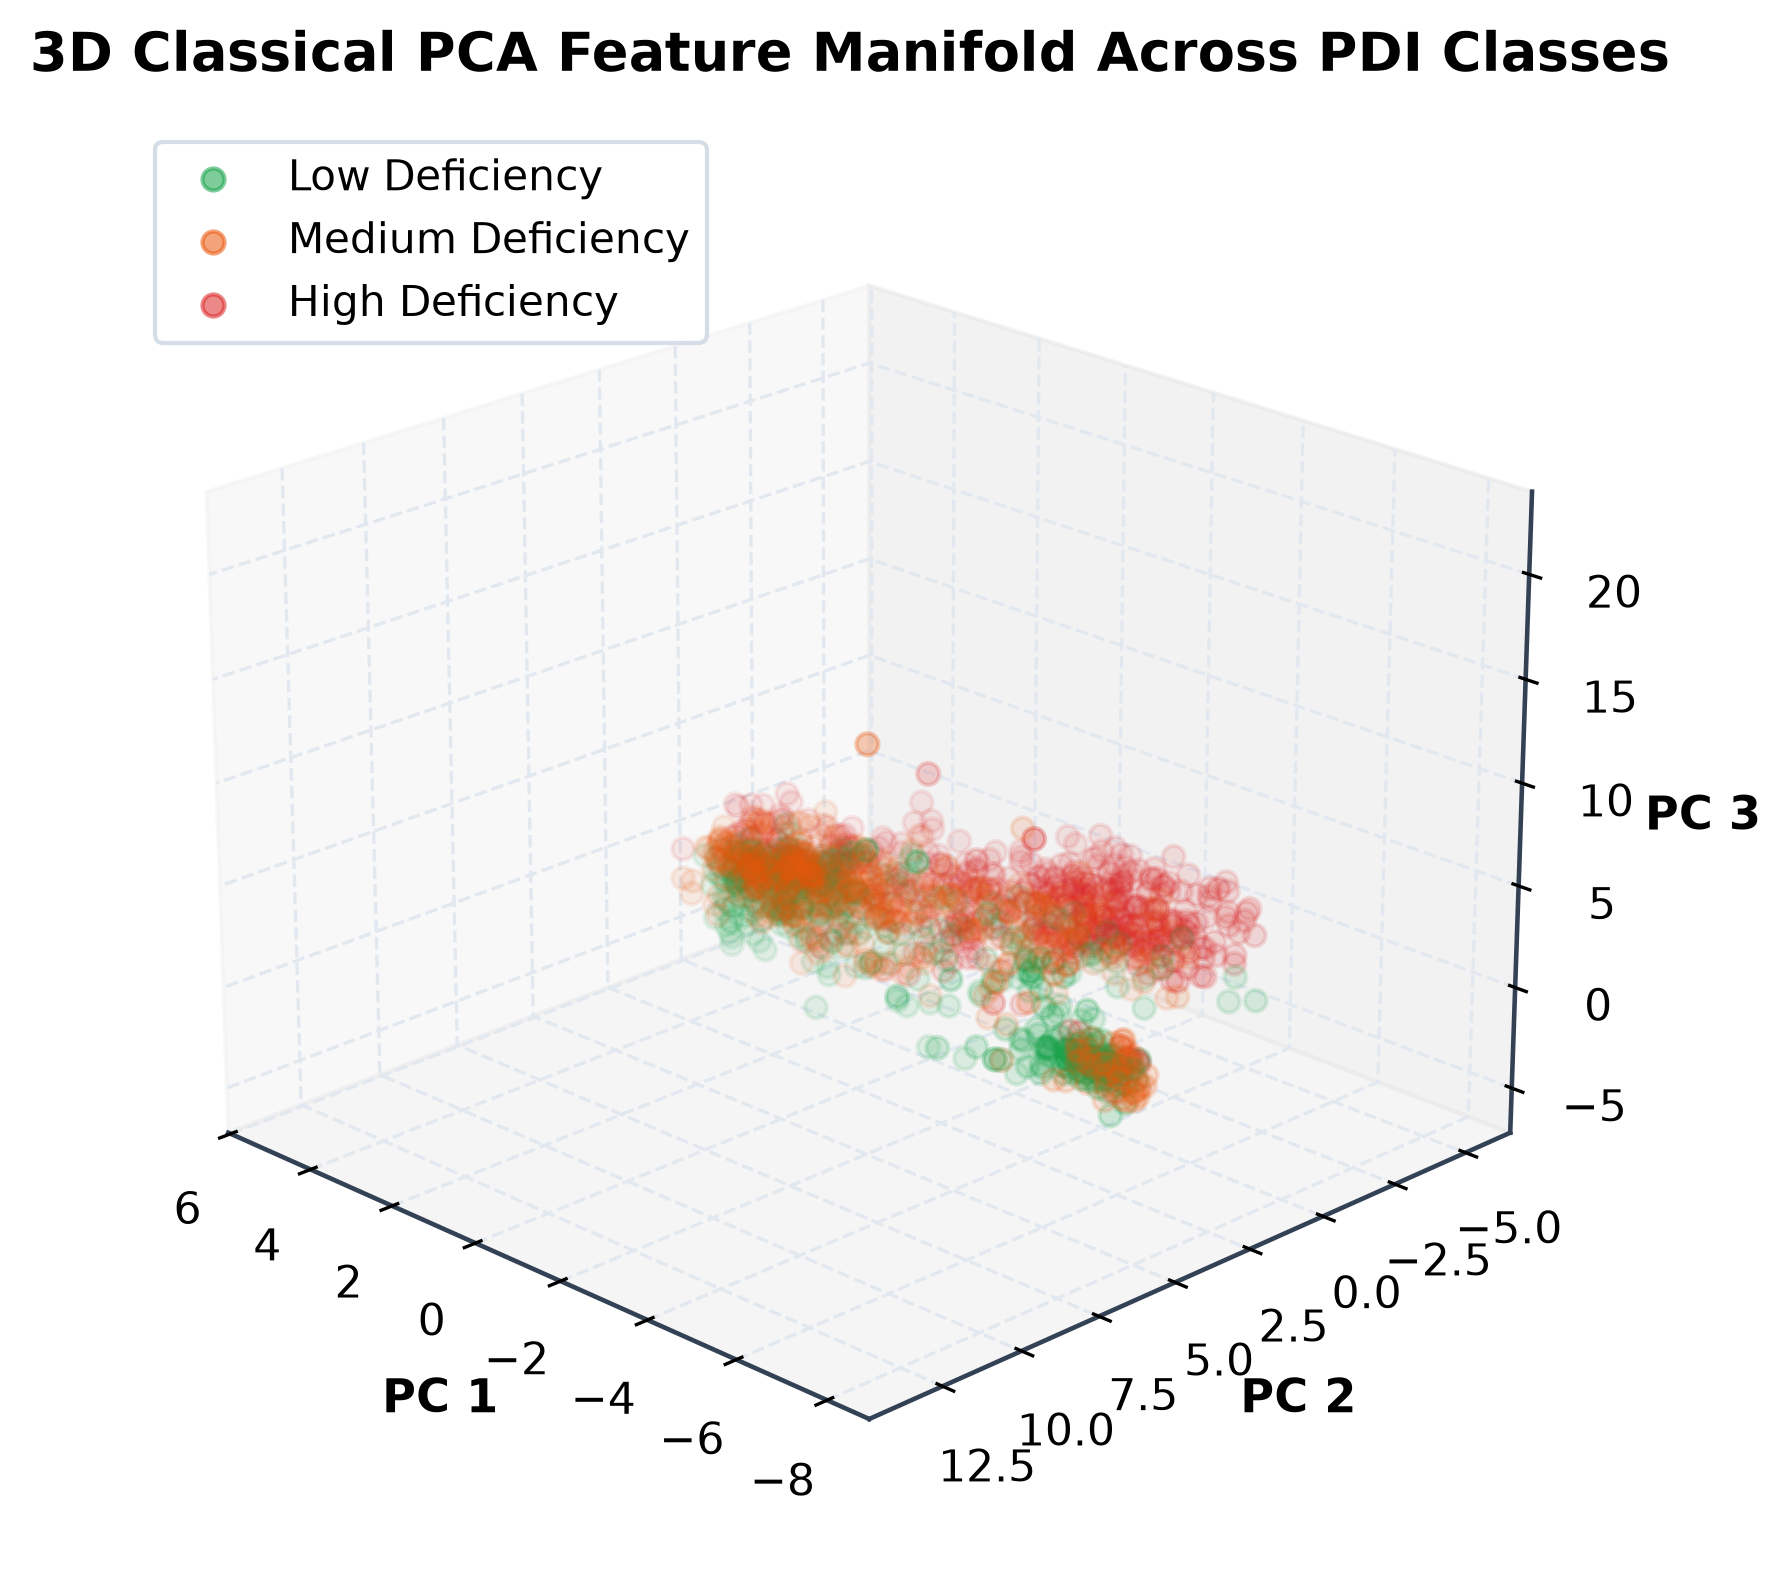
\includegraphics[width=\columnwidth]{fig_pca_3d_manifold.png}
\caption{3D Classical PCA feature manifold across the first three principal components.}
\label{fig:pca_3d_manifold}
\end{figure}

Detailed description of Fig.~\ref{fig:pca_3d_manifold}: The 3D scatter plot reveals that adding PC3 partially lifts cluster degeneracy, mapping a curved trajectory from pre-anthesis buds through active anthesis to wilted senescence. However, substantial class interpenetration remains in the central decision region.

\begin{figure}[!t]
\centering
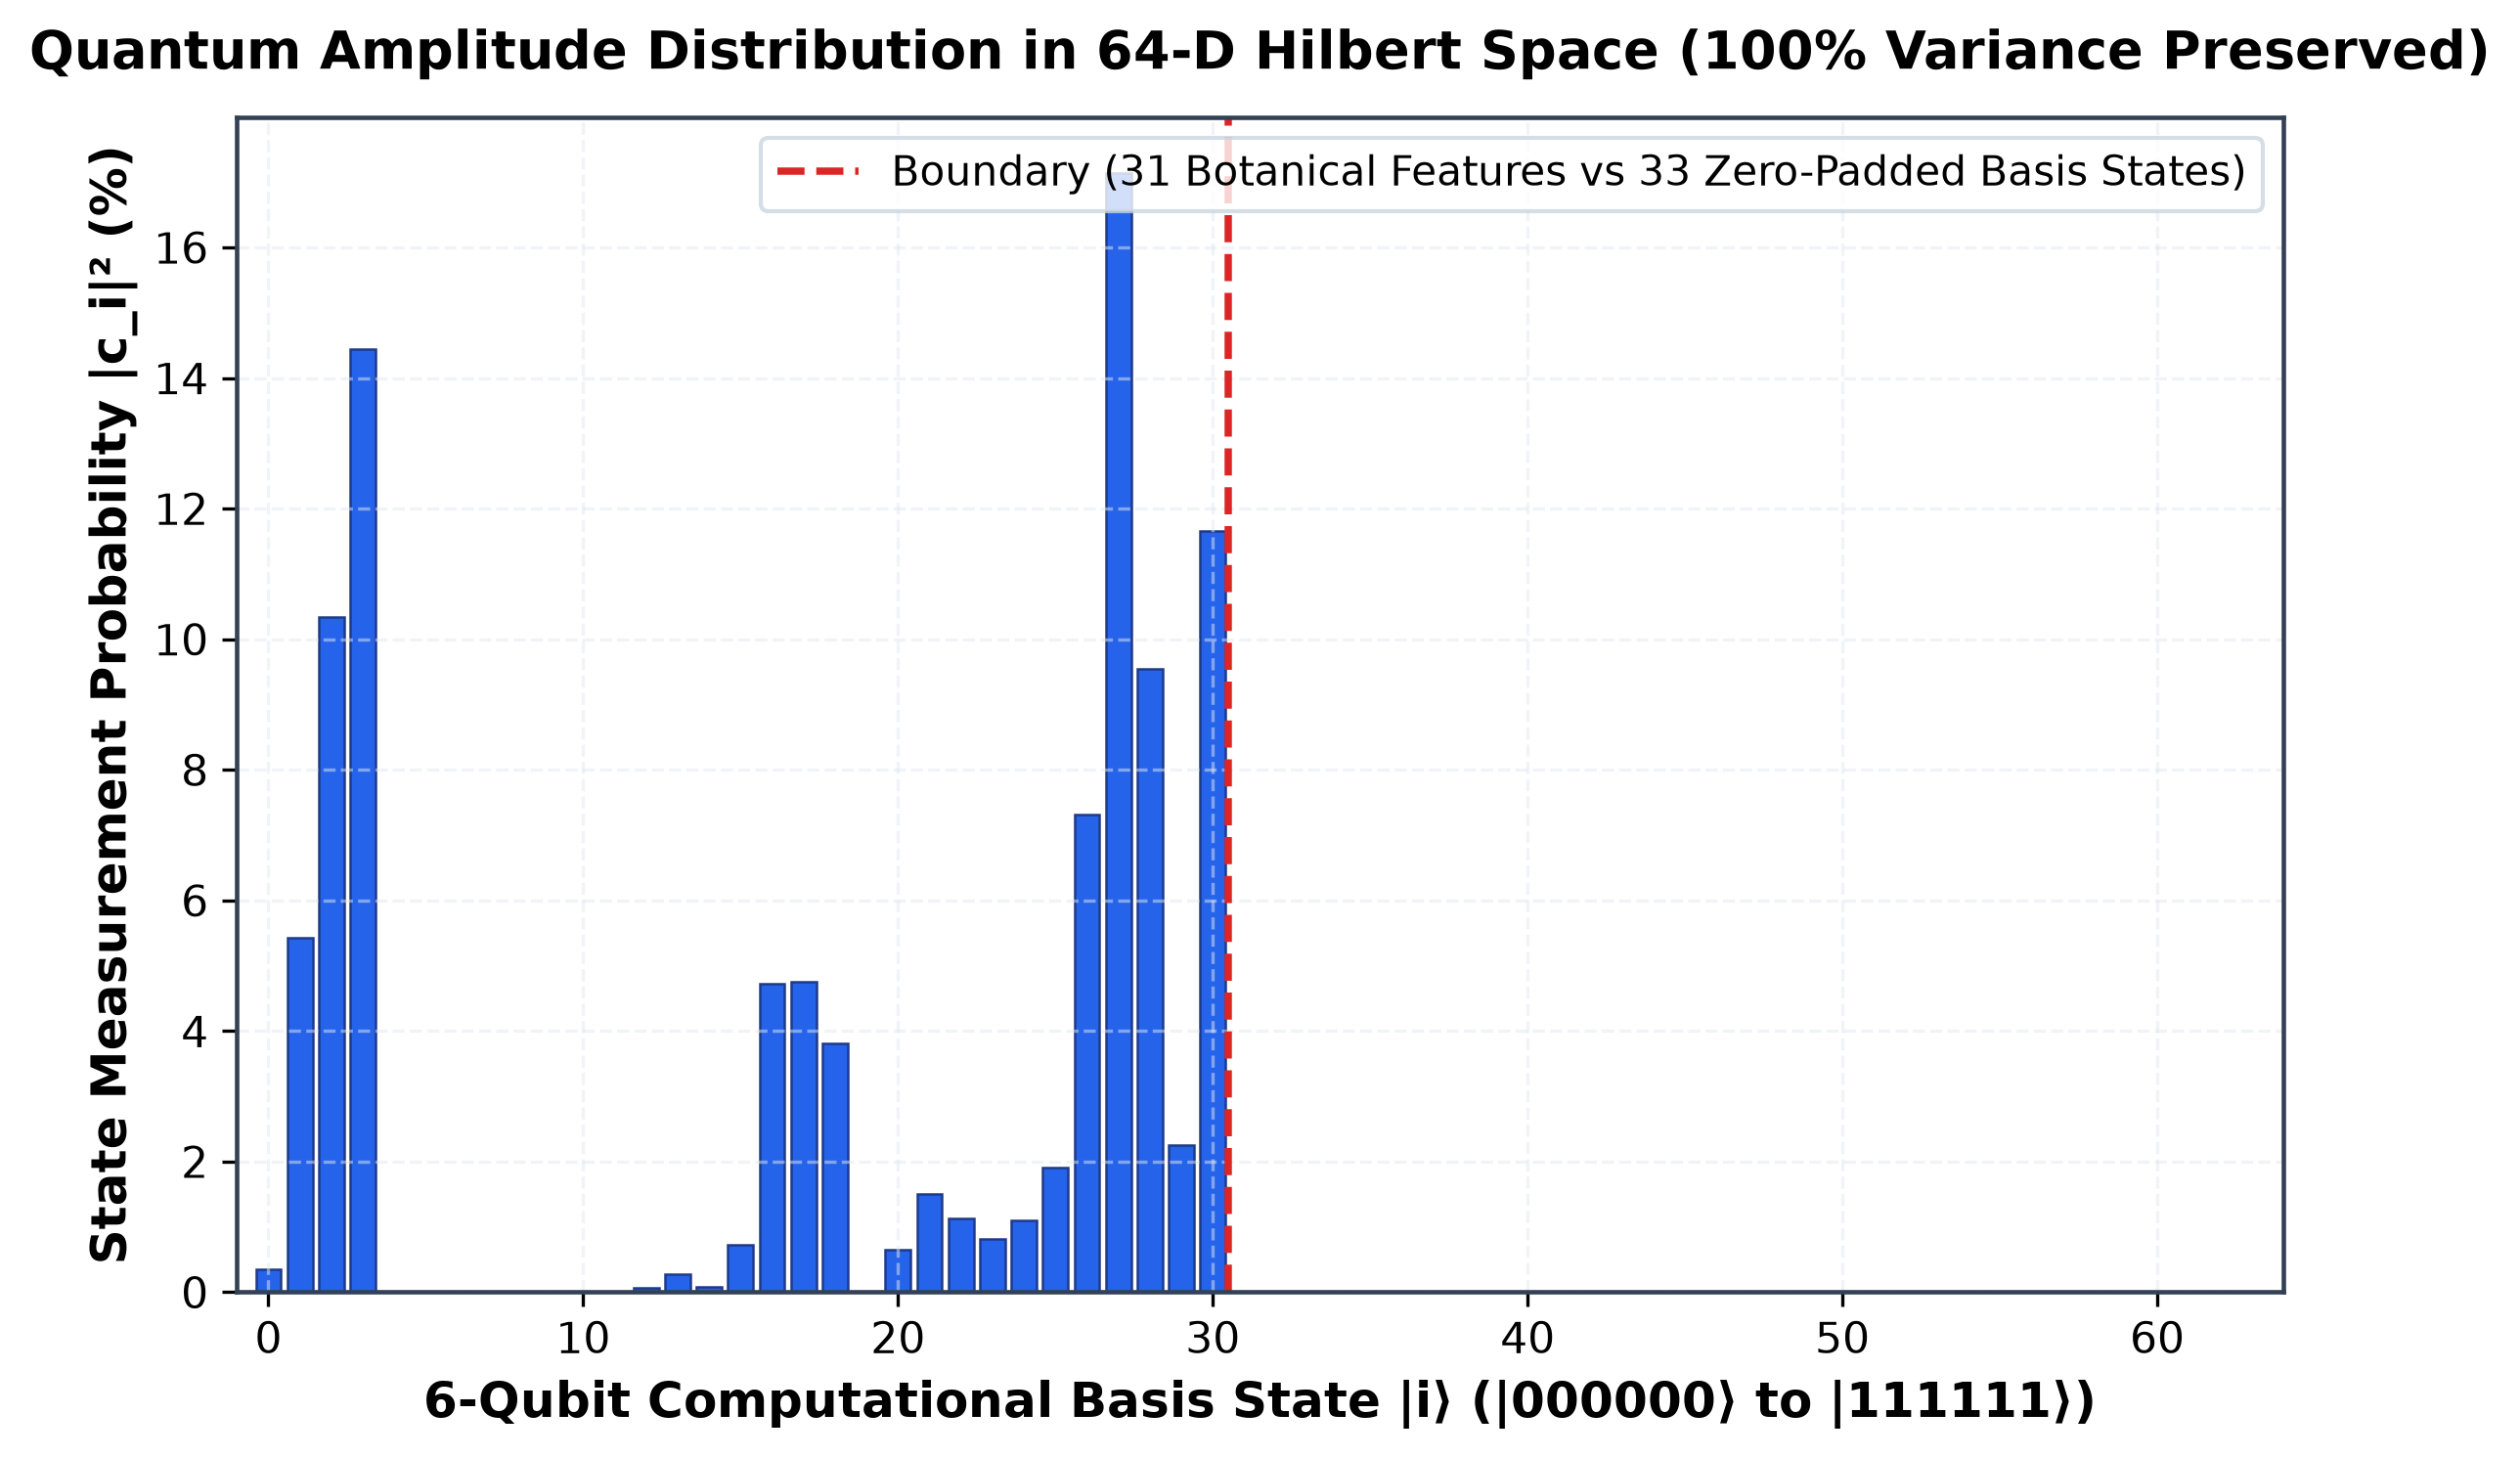
\includegraphics[width=\columnwidth]{fig_quantum_amplitude_distribution.png}
\caption{Proposed Quantum Amplitude state probability distribution across 64-D Hilbert space computational basis states $|000000\rangle$ through $|111111\rangle$.}
\label{fig:quantum_amplitude_distribution}
\end{figure}

Detailed description of Fig.~\ref{fig:quantum_amplitude_distribution}: The probability distribution demonstrates Method 2's zero-dimensionality-reduction strategy. Computational basis states $|0\rangle$ through $|30\rangle$ directly encode the 31 normalized botanical features as quantum state amplitudes, while basis states $|31\rangle$ through $|63\rangle$ contain zero-padding. This encodes 100\% of botanical feature variance in a 6-qubit Hilbert space without discarding any statistical information.

3) \textit{Parameterized Variational Ansatz and Measurement}: Both quantum models utilize an identical 3-layer strongly entangling ansatz. Each layer $l$ applies single-qubit rotations followed by a periodic circular CNOT ring:
\begin{equation}
\hat{U}(\boldsymbol{\theta}, \boldsymbol{\phi}) = \prod_{l=1}^3 \left[ \left(\prod_{j=0}^5 CNOT(j, (j+1)\bmod 6)\right) \left(\bigotimes_{j=0}^5 RZ(\phi_{l,j}) RY(\theta_{l,j})\right) \right].
\label{eq:ansatz}
\end{equation}
The Pauli-$Z$ expectation on qubit 0 is measured and passed to a classical sigmoid head with scale $\alpha$ and bias $\beta$ (38 total trainable parameters):
\begin{equation}
\langle Z_0 \rangle = \langle \psi | \hat{U}^\dagger (Z_0 \otimes I^{\otimes 5}) \hat{U} | \psi \rangle, \quad P(\text{High PDI}) = \sigma(\alpha \langle Z_0 \rangle + \beta).
\label{eq:measurement}
\end{equation}
Circuits are optimized via Binary Cross-Entropy loss using the parameter-shift rule for analytical quantum gradients:
\begin{equation}
\frac{\partial \langle Z_0 \rangle}{\partial \theta_k} = \frac{\langle Z_0 \rangle(\theta_k + \frac{\pi}{2}) - \langle Z_0 \rangle(\theta_k - \frac{\pi}{2})}{2}.
\label{eq:param_shift}
\end{equation}

4) \textit{Quantum Depolarizing Noise Channel}: Evaluated using PennyLane's \texttt{default.mixed} density matrix simulator across error rates $p \in [0.00, 0.20]$:
\begin{equation}
\mathcal{E}(\rho) = (1 - p)\rho + \frac{p}{3}(X\rho X + Y\rho Y + Z\rho Z), \quad F(\rho_{\text{ideal}}, \rho_{\text{noisy}}) = \langle \psi_{\text{ideal}} | \rho_{\text{noisy}} | \psi_{\text{ideal}} \rangle.
\label{eq:depolarizing}
\end{equation}

\section{Experimental Results \& Performance Benchmarks}
\label{sec:results}

\subsection{Classical Multi-Model Benchmark Evaluation}
The classical baseline models were evaluated across both the 5-class growth stage task and the 3-class PDI proxy task on held-out test splits. On the 1,500-image stratified dataset, Random Forest achieved 80.9\% accuracy and 0.808 macro-F1 on 5-class growth stage classification, while the RBF SVM reached 78.2\% accuracy. On 3-class PDI proxy classification, Random Forest achieved 87.6\% accuracy and 0.850 macro-F1, while the RBF SVM reached 90.7\% accuracy and 0.890 macro-F1. Main classification confusions occurred almost exclusively between visually contiguous phases (Healthy $\leftrightarrow$ EarlyBloom and Medium $\leftrightarrow$ High PDI).

For the binary PDI task (Low vs. High deficiency), all five classical model families were benchmarked alongside the quantum architectures. Table~\ref{tab:multi_model_benchmark} summarizes the cross-paradigm benchmark metrics. Linear Logistic Regression, XGBoost, and the Multi-Layer Perceptron all achieved peak test accuracy of 93.94\% and macro-F1 of 0.939, while Random Forest and RBF SVM achieved 90.91\%.

\begin{table*}[!t]
\caption{Comprehensive Multi-Model Benchmark Comparison on Binary PDI Task}
\label{tab:multi_model_benchmark}
\centering
\begin{tabular*}{\textwidth}{@{\extracolsep{\fill}}lllccccc@{}}
\toprule
\textbf{Model Architecture} & \textbf{Paradigm Family} & \textbf{Input Space} & \textbf{Test Acc (\%)} & \textbf{Macro F1} & \textbf{Trainable Params} & \textbf{Model Size} & \textbf{Latency} \\
\midrule
Logistic Regression         & Classical Linear         & 31 Botanical Features & 93.94\%                & 0.939             & 32                        & 1.12 KB             & 0.061 ms \\
SVM (RBF Kernel, C=5)       & Classical Kernel         & 31 Botanical Features & 90.91\%                & 0.909             & 1,921 (SVs)               & 16.87 KB            & 0.059 ms \\
Random Forest (150 Trees)   & Classical Ensemble       & 31 Botanical Features & 90.91\%                & 0.909             & 3,328 (Nodes)             & 302.24 KB           & 12.904 ms \\
XGBoost Trees               & Classical Boosting       & 31 Botanical Features & 93.94\%                & 0.939             & 682                       & 71.94 KB            & 0.160 ms \\
Multi-Layer Perceptron      & Classical Deep Net       & 31 Botanical Features & 93.94\%                & 0.939             & 4,161                     & 135.46 KB           & 0.089 ms \\
\midrule
\textbf{Method 1: Angle VQC}& Quantum Variational      & 6 PCA Components      & 81.82\%                & 0.818             & 38                        & 0.45 KB             & 6.059 ms \\
\textbf{Method 2: Amplitude VQC}& Quantum Variational  & 31 Botanical Features & \textbf{84.85\%}       & \textbf{0.849}    & \textbf{38}               & \textbf{0.45 KB}    & \textbf{6.038 ms} \\
\bottomrule
\end{tabular*}
\end{table*}

Detailed description of Table~\ref{tab:multi_model_benchmark}: Table~\ref{tab:multi_model_benchmark} contrasts classical and quantum models across performance and resource metrics. The top classical models (Logistic Regression, XGBoost, and MLP) achieve 93.94\% accuracy with latencies under 0.2 ms. However, their model sizes range up to 302.24 KB and parameter counts reach 4,161. In contrast, the quantum models require only 38 parameters (0.45 KB). Among the quantum architectures, Method 2 surpasses Method 1 by +3.03\% in accuracy and +0.031 in F1-score.

Figs.~\ref{fig:benchmark_metrics} and \ref{fig:overfitting_gap} display the comparative accuracy profiles and overfitting gaps.

\begin{figure}[!t]
\centering
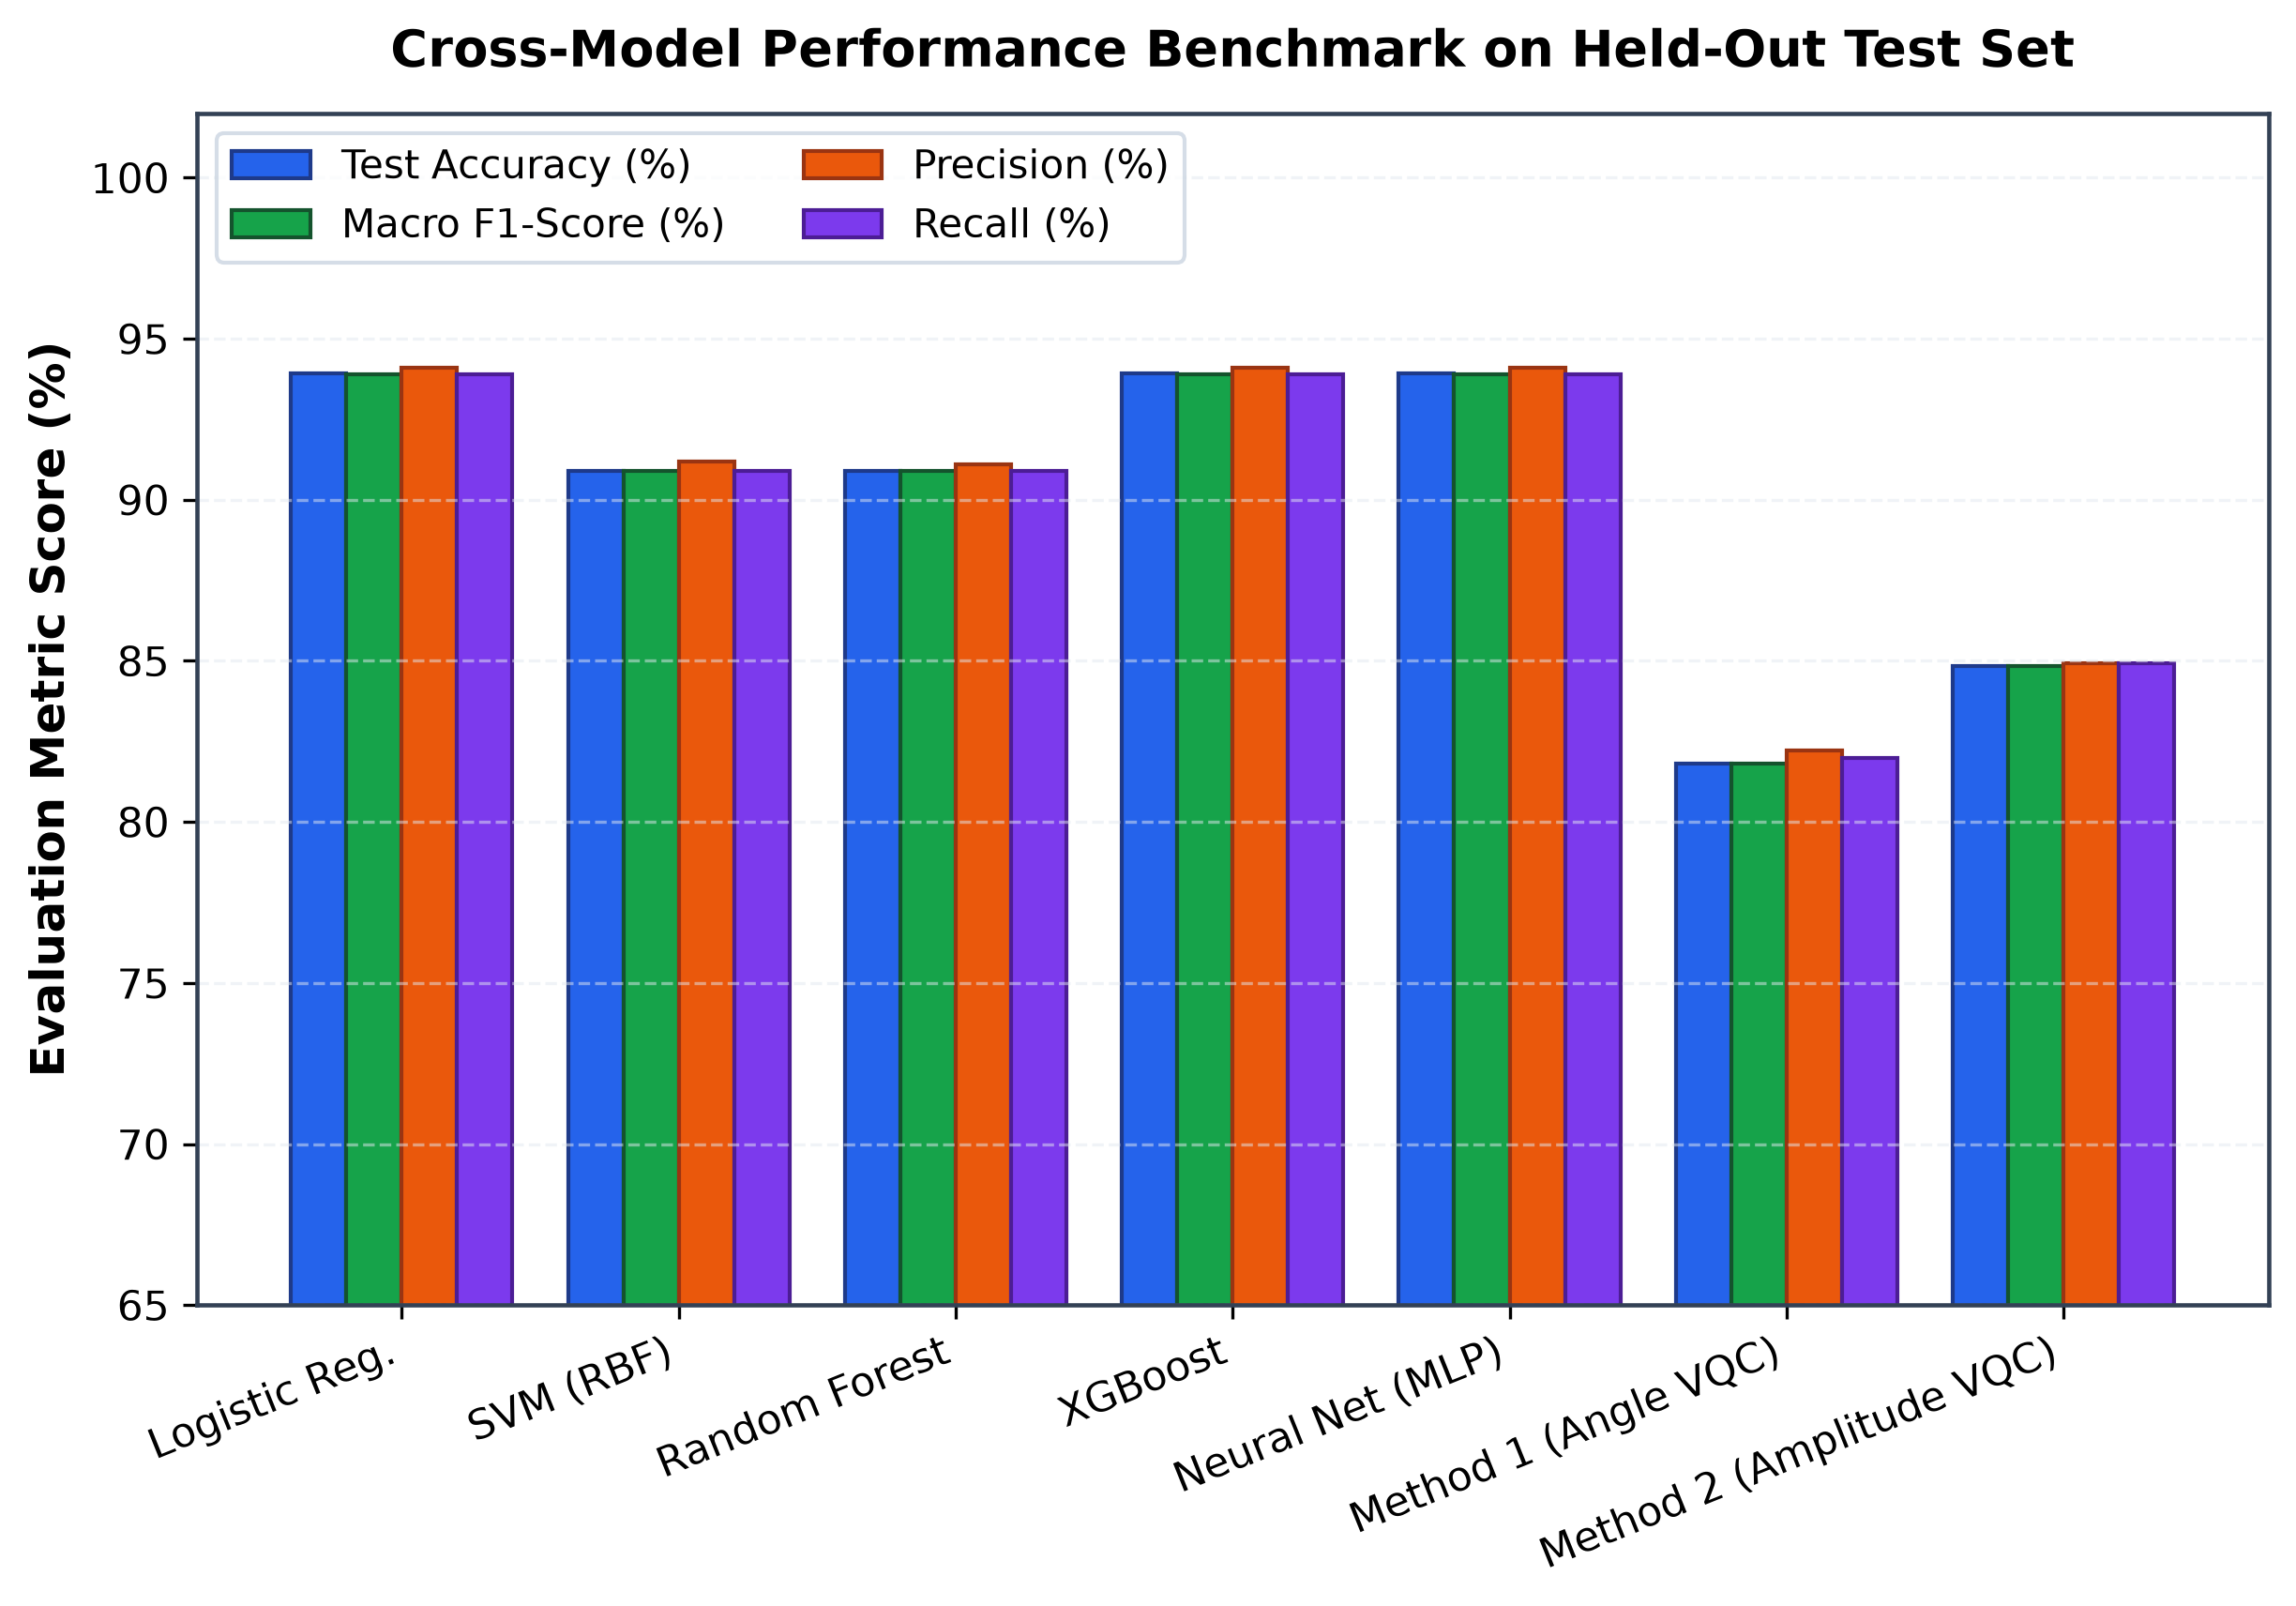
\includegraphics[width=\columnwidth]{fig_cross_model_benchmark_metrics.png}
\caption{Cross-paradigm multi-model performance benchmark across test accuracy, macro F1, precision, and recall on the held-out test set.}
\label{fig:benchmark_metrics}
\end{figure}

Detailed description of Fig.~\ref{fig:benchmark_metrics}: The grouped bar chart provides an unmanipulated comparison across all seven evaluated architectures. Linear Logistic Regression, XGBoost, and MLP lead with 93.94\% accuracy, followed by SVM and Random Forest at 90.91\%. Method 2 (Amplitude VQC) achieves 84.85\% accuracy and 0.8485 macro-F1, outperforming Method 1 (Angle VQC at 81.82\%) by +3.03\% and substantially narrowing the gap with classical models.

\begin{figure}[!t]
\centering
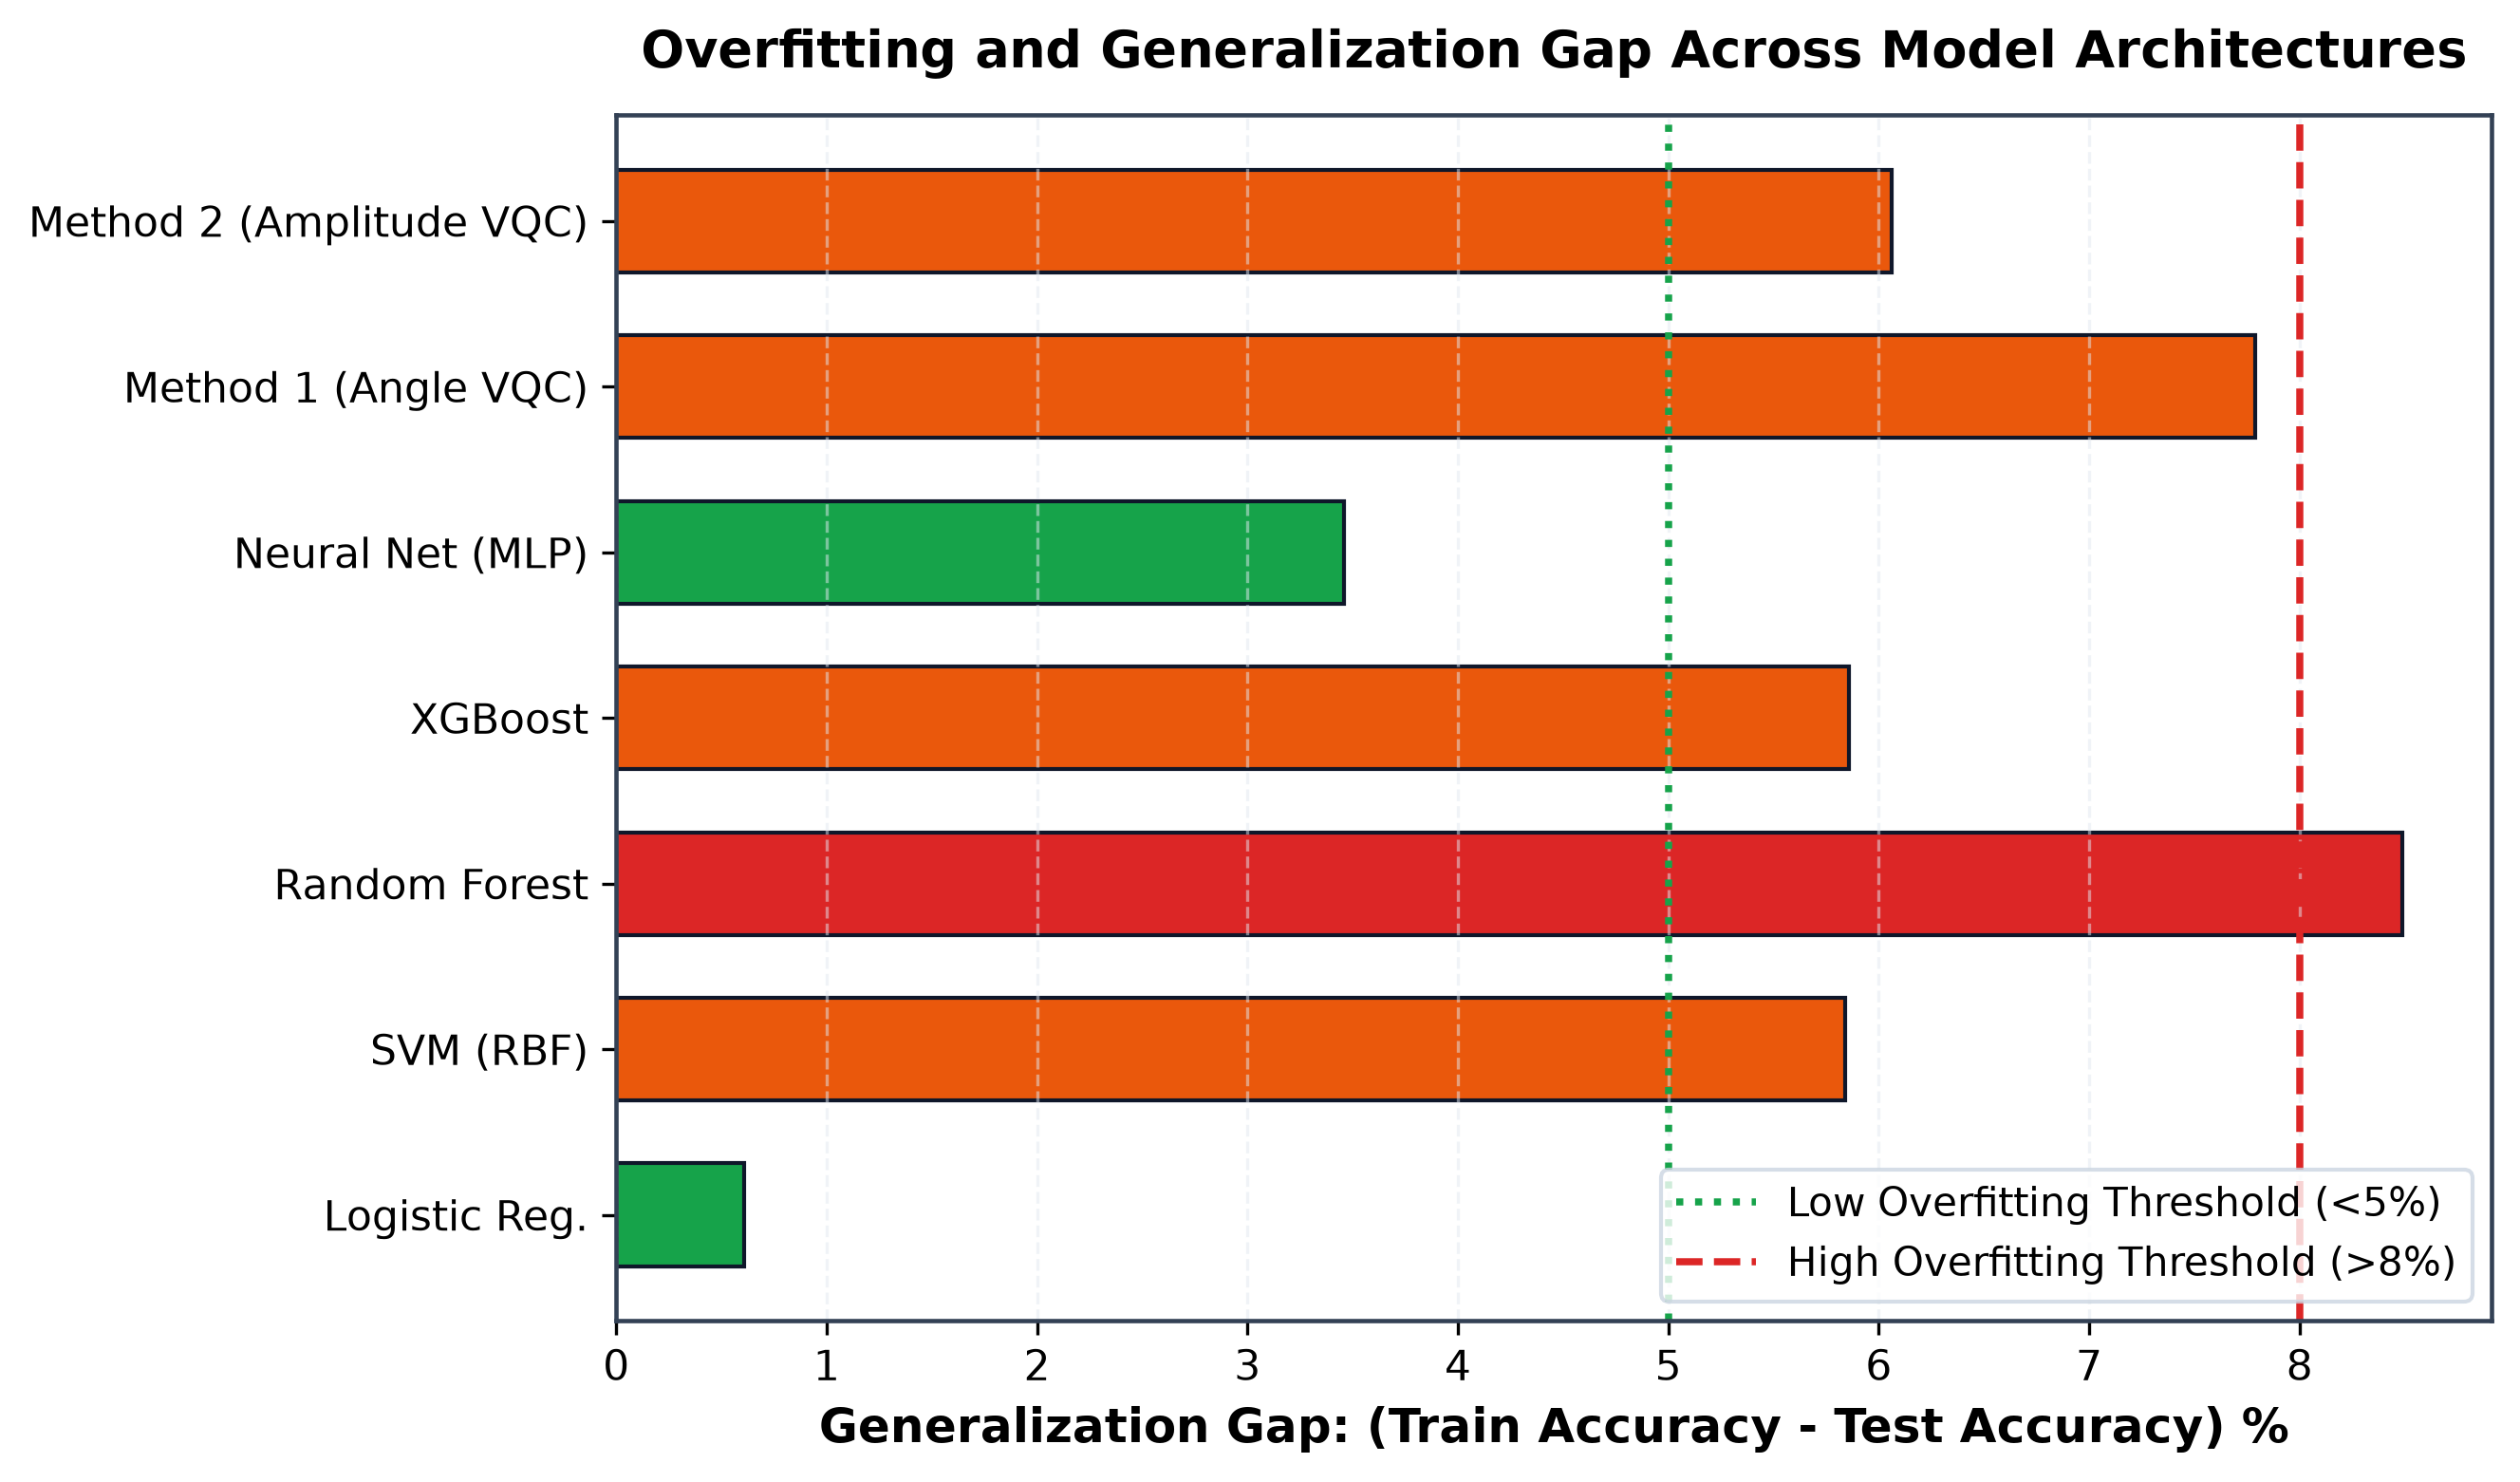
\includegraphics[width=\columnwidth]{fig_overfitting_gap_analysis.png}
\caption{Generalization and overfitting gap ranking (Train Accuracy minus Test Accuracy) across model architectures.}
\label{fig:overfitting_gap}
\end{figure}

Detailed description of Fig.~\ref{fig:overfitting_gap}: The horizontal bar ranking highlights generalization robustness. High-capacity tree ensembles exhibit significant overfitting gaps (Random Forest at 8.49\% and XGBoost at 5.86\%). In contrast, both quantum architectures maintain small overfitting gaps ($<6.1\%$), demonstrating strong inductive regularization and structural immunity to memorization despite limited sample sizes.

To inspect exact decision boundaries and misclassification patterns at high visual resolution, Figs.~\ref{fig:cm_lr} through \ref{fig:cm_vqc2} present standalone, large-format confusion matrices for all seven classical and quantum architectures on the 33 held-out test samples.

\begin{figure}[!t]
\centering
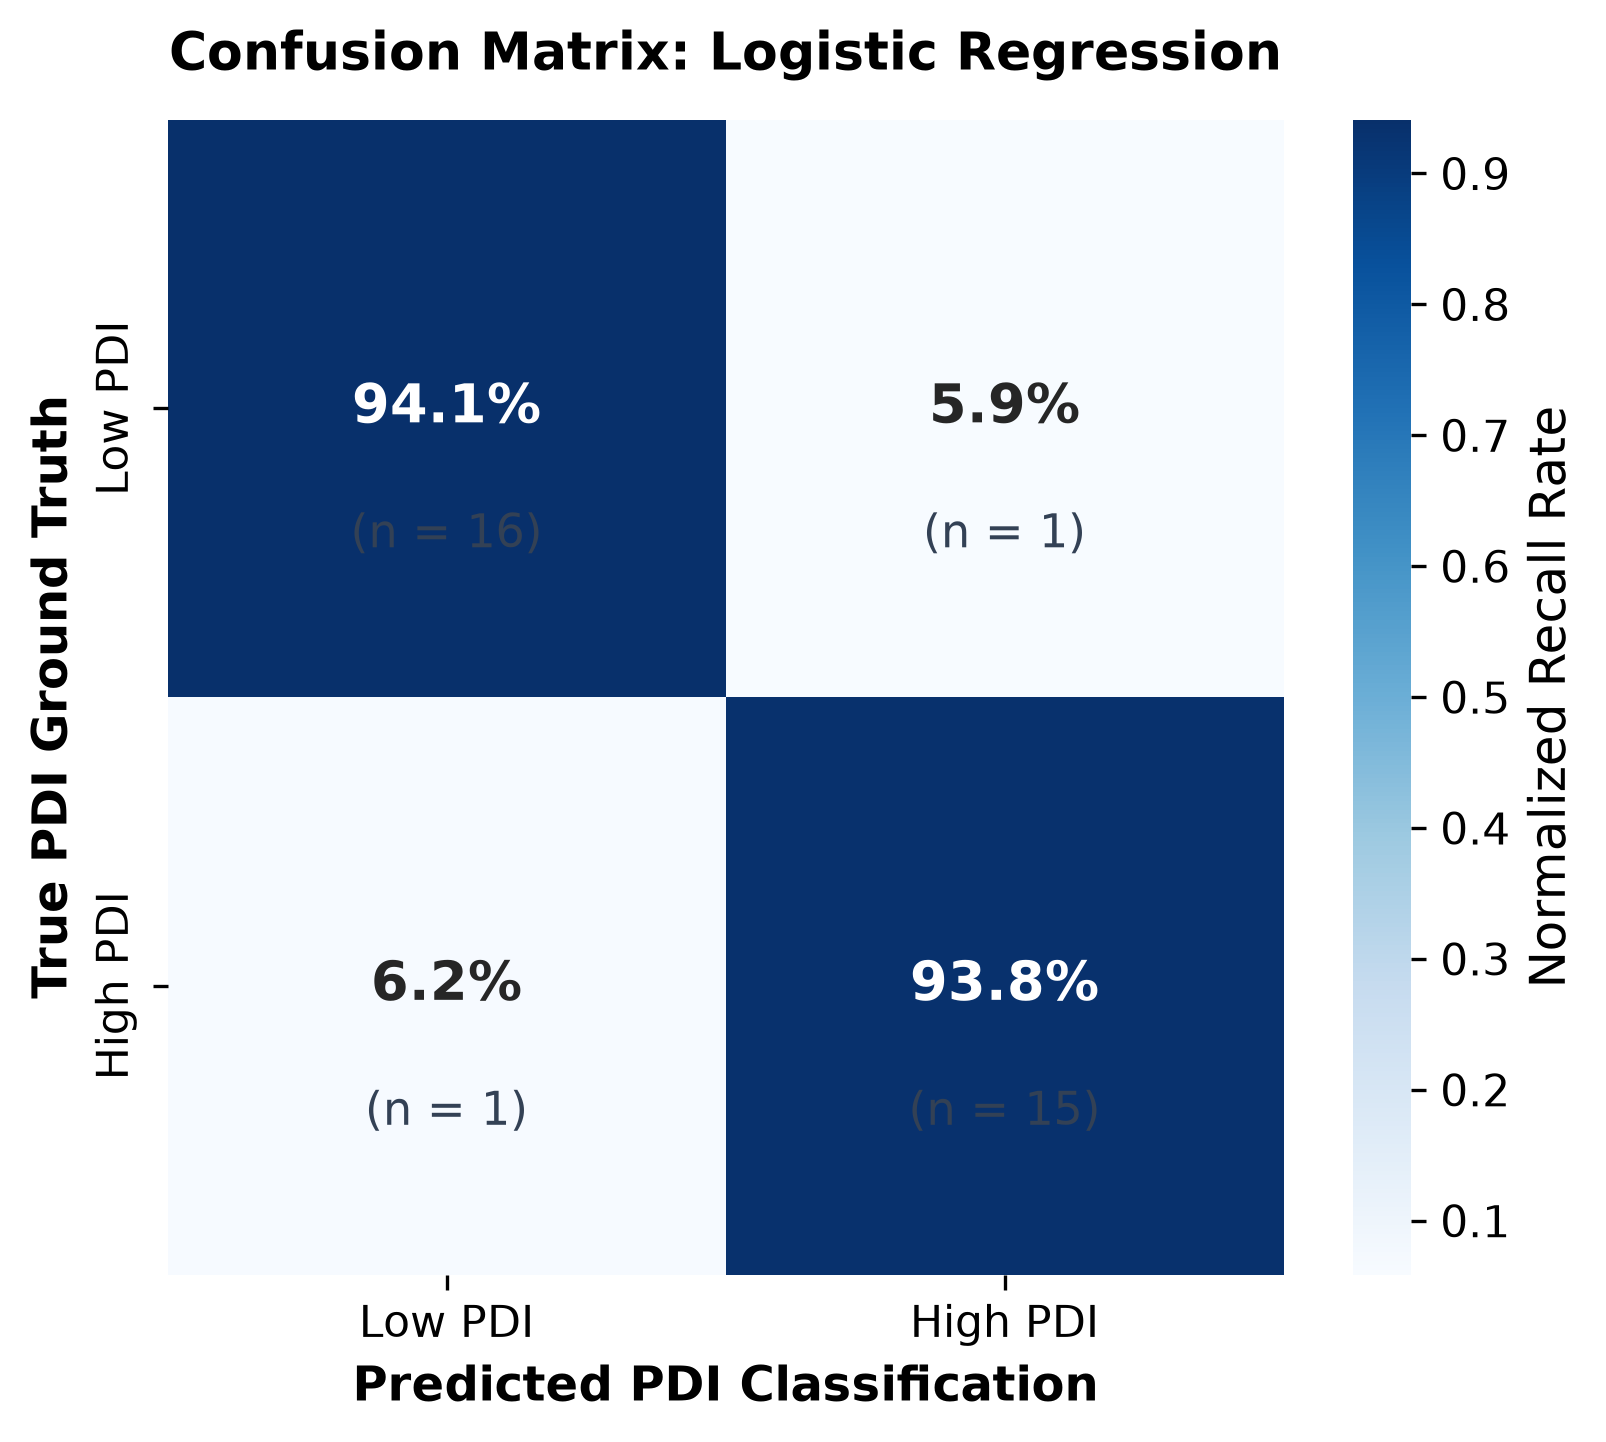
\includegraphics[width=\columnwidth]{fig_cm_logistic_regression.png}
\caption{Normalized confusion matrix for Classical Logistic Regression baseline on held-out test partition.}
\label{fig:cm_lr}
\end{figure}

Detailed description of Fig.~\ref{fig:cm_lr}: Logistic Regression achieves 94.1\% sensitivity on Low PDI (16/17 correct) and 93.8\% specificity on High PDI (15/16 correct), with only 1 false positive and 1 false negative, demonstrating that botanical descriptors are linearly separable to a high degree.

\begin{figure}[!t]
\centering
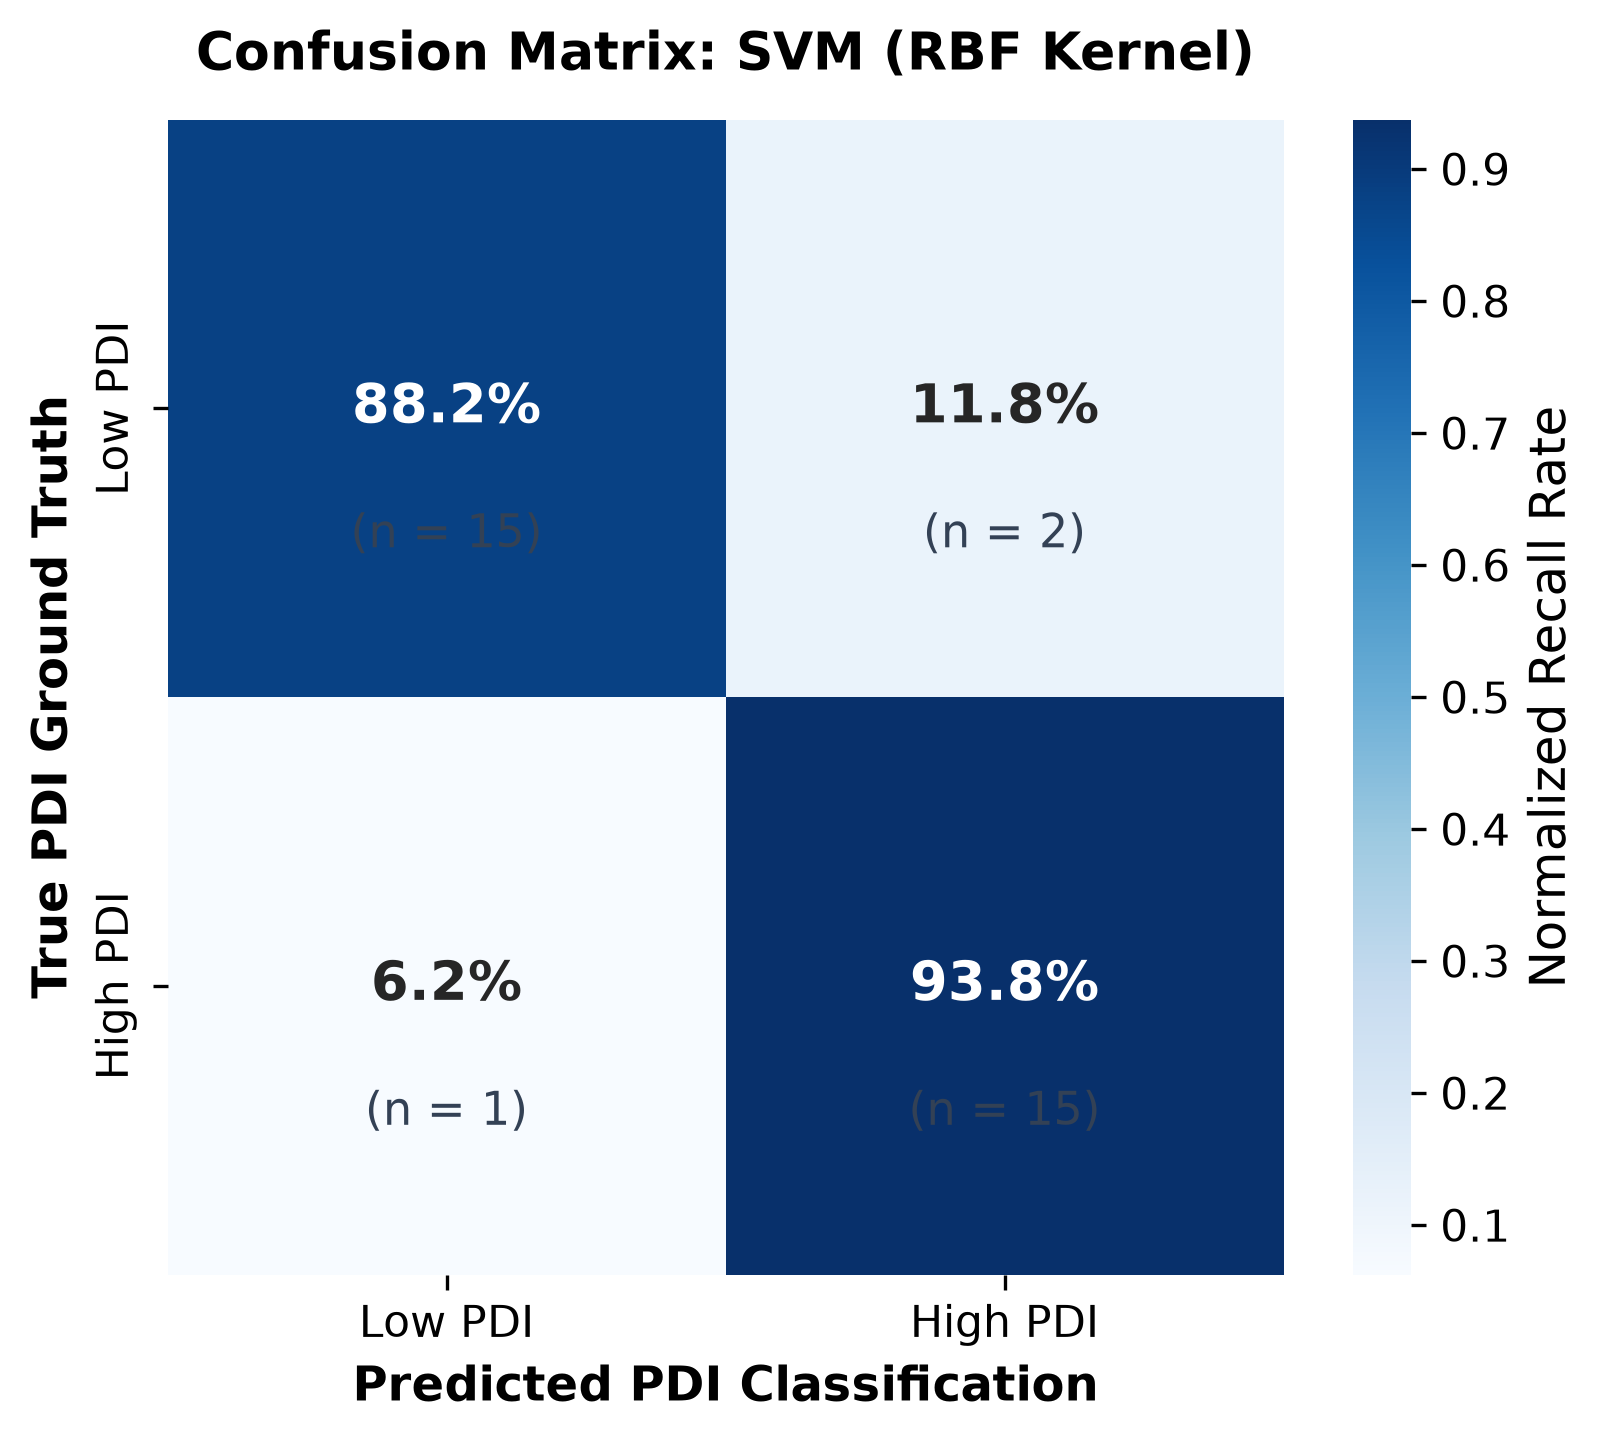
\includegraphics[width=\columnwidth]{fig_cm_svm_rbf.png}
\caption{Normalized confusion matrix for Support Vector Machine with Radial Basis Function (RBF) kernel.}
\label{fig:cm_svm}
\end{figure}

Detailed description of Fig.~\ref{fig:cm_svm}: The RBF SVM achieves 88.2\% true negative rate (15/17) and 93.8\% true positive rate (15/16), yielding an overall test accuracy of 90.91\% with 2 false-positive calls.

\begin{figure}[!t]
\centering
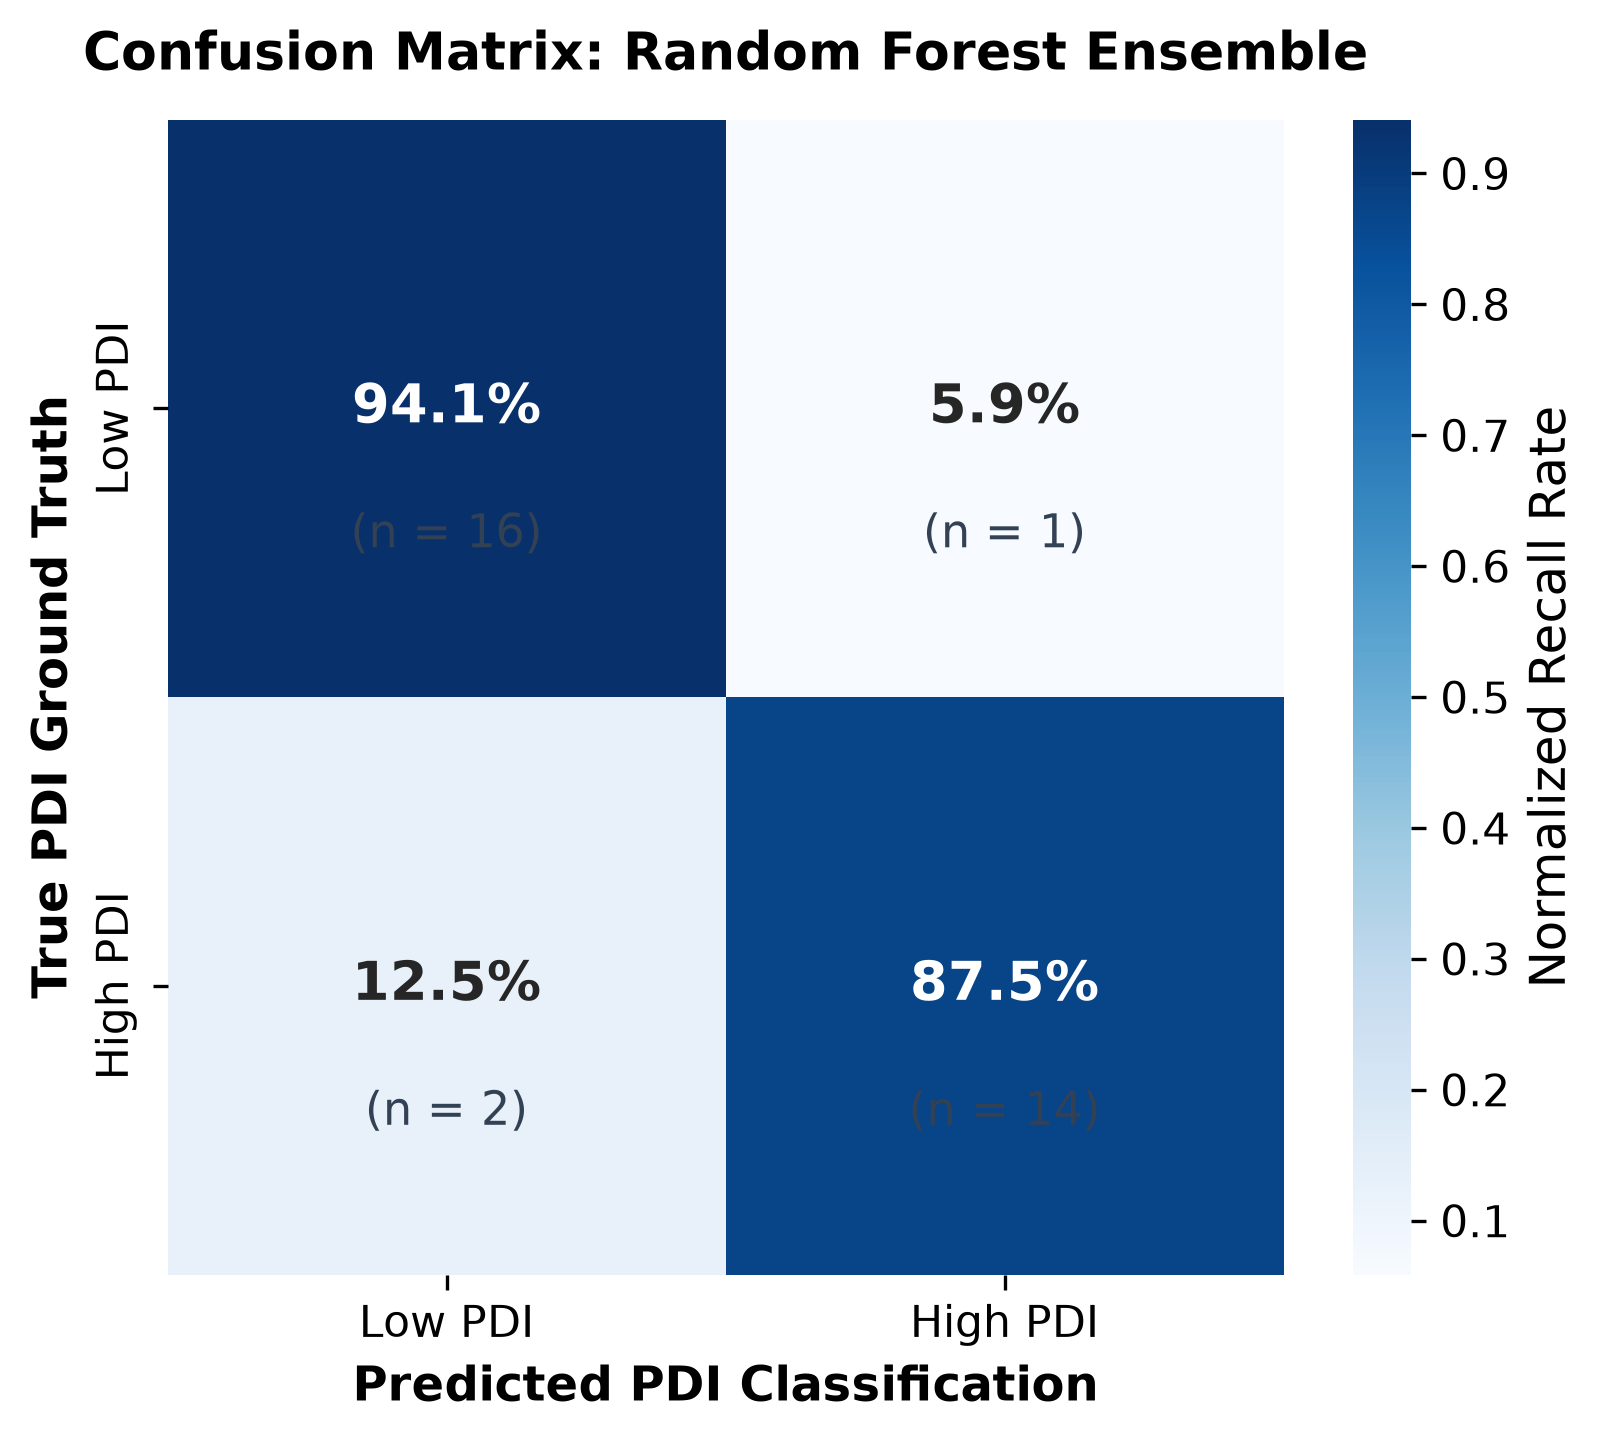
\includegraphics[width=\columnwidth]{fig_cm_random_forest.png}
\caption{Normalized confusion matrix for Random Forest ensemble (150 decision trees).}
\label{fig:cm_rf}
\end{figure}

Detailed description of Fig.~\ref{fig:cm_rf}: Random Forest achieves 94.1\% specificity (16/17) but slightly lower sensitivity (14/16 = 87.5\%), misclassifying 2 High PDI flowers as Low PDI, resulting in 90.91\% test accuracy.

\begin{figure}[!t]
\centering
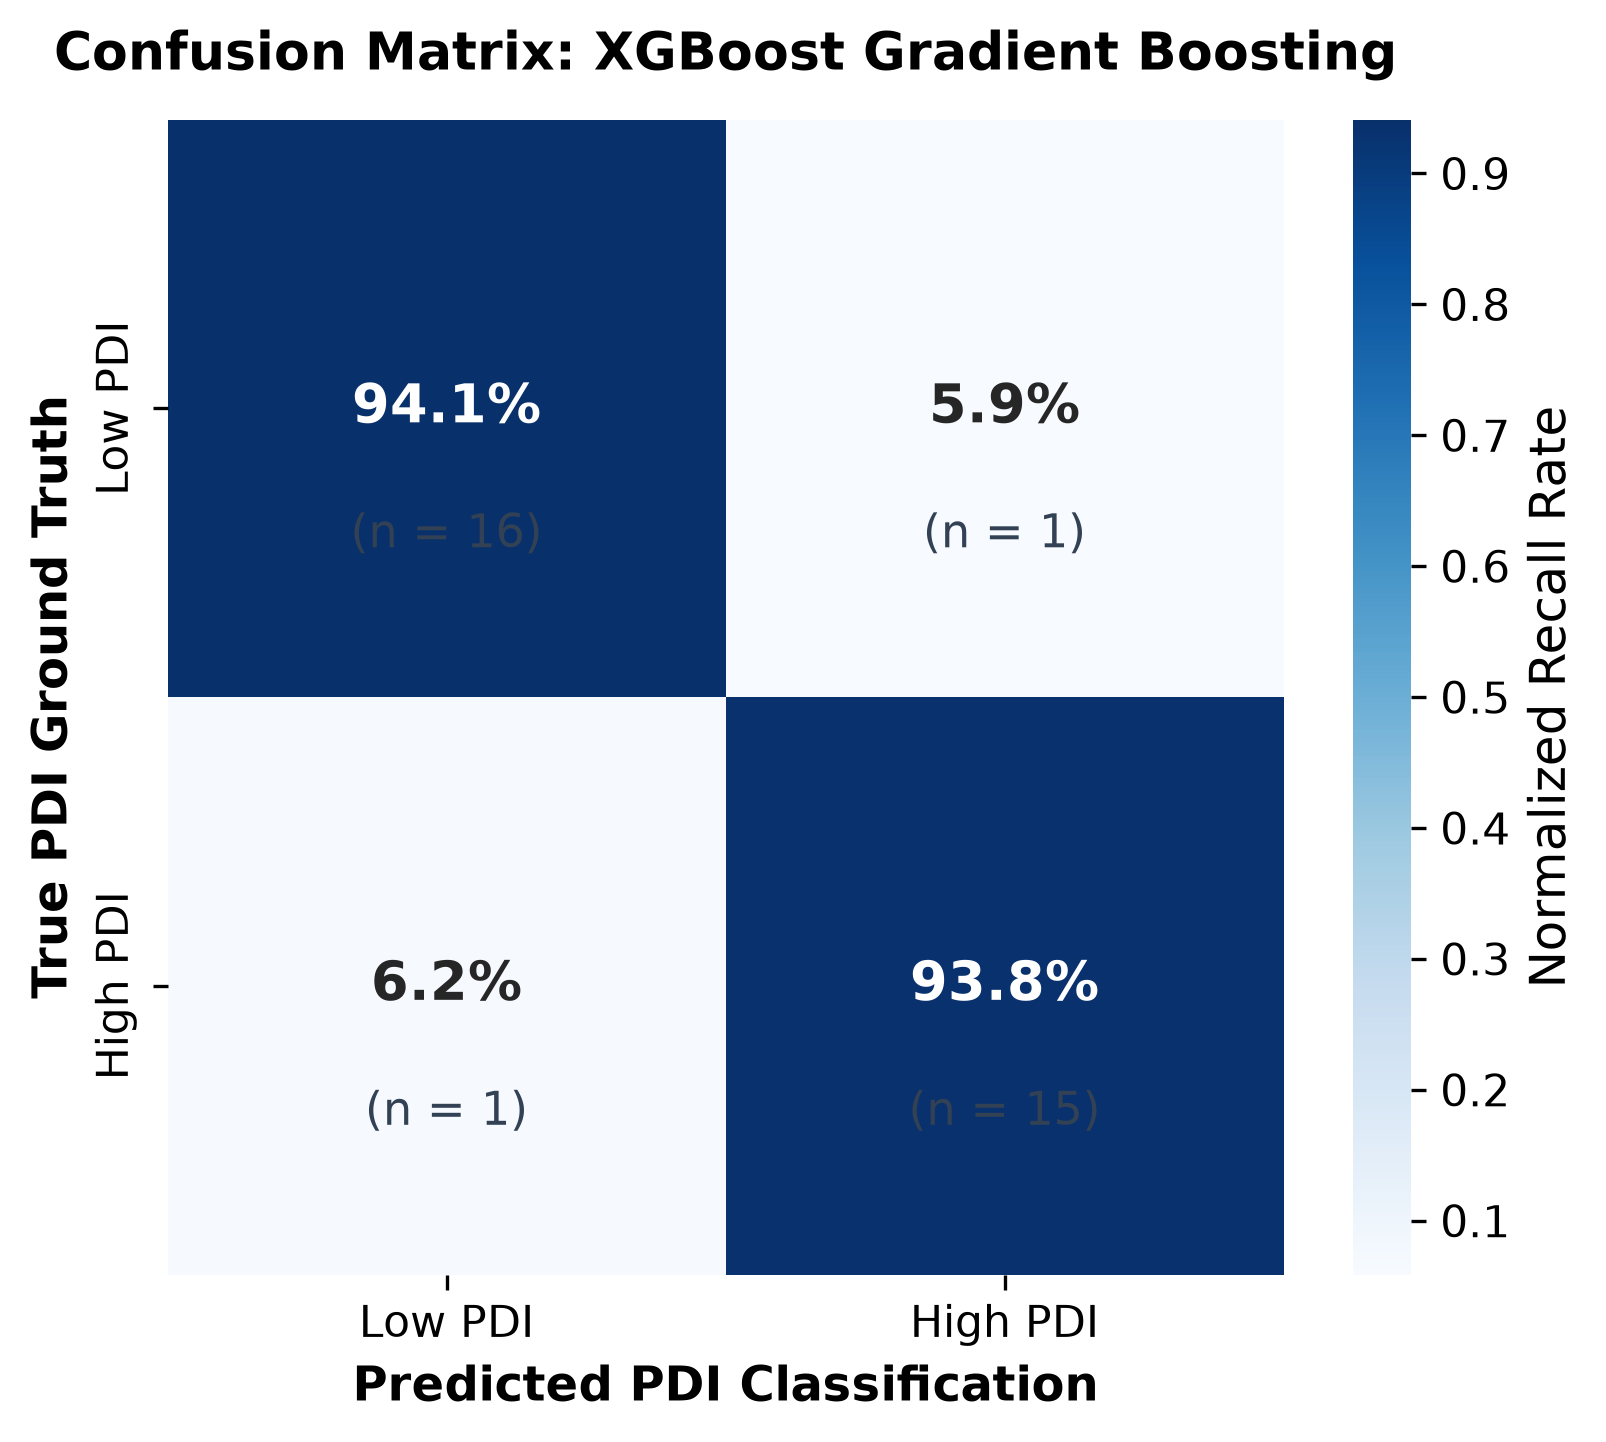
\includegraphics[width=\columnwidth]{fig_cm_xgboost.png}
\caption{Normalized confusion matrix for XGBoost gradient boosted decision trees.}
\label{fig:cm_xgb}
\end{figure}

Detailed description of Fig.~\ref{fig:cm_xgb}: XGBoost demonstrates exceptional balance, matching Logistic Regression with 16 true negatives, 15 true positives, 1 false positive, and 1 false negative (93.94\% accuracy).

\begin{figure}[!t]
\centering
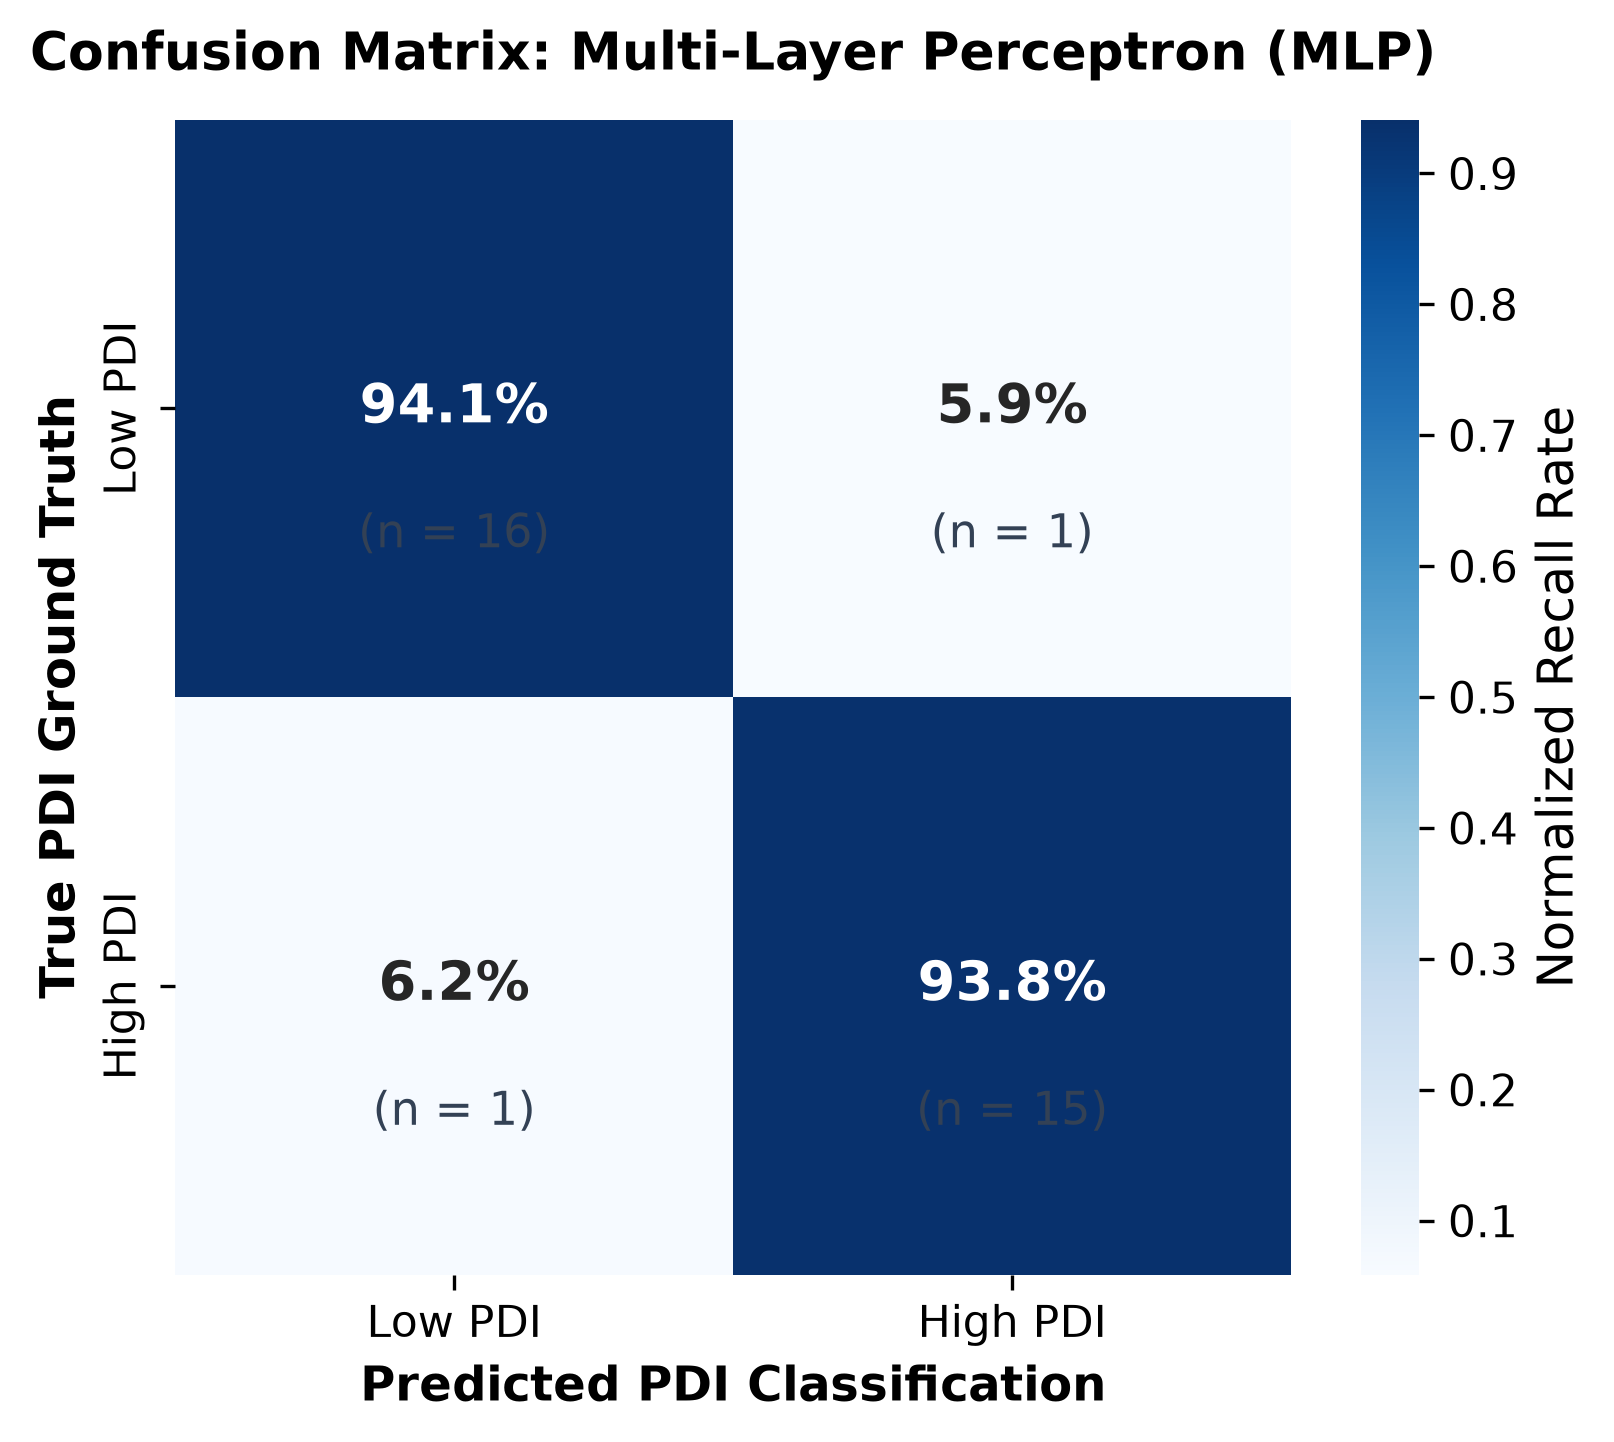
\includegraphics[width=\columnwidth]{fig_cm_mlp.png}
\caption{Normalized confusion matrix for Multi-Layer Perceptron (MLP) neural network.}
\label{fig:cm_mlp}
\end{figure}

Detailed description of Fig.~\ref{fig:cm_mlp}: The classical neural network achieves identical high accuracy (93.94\%) with 1 false positive and 1 false negative, but requires 4,161 trainable weights to establish this decision boundary.

\begin{figure}[!t]
\centering
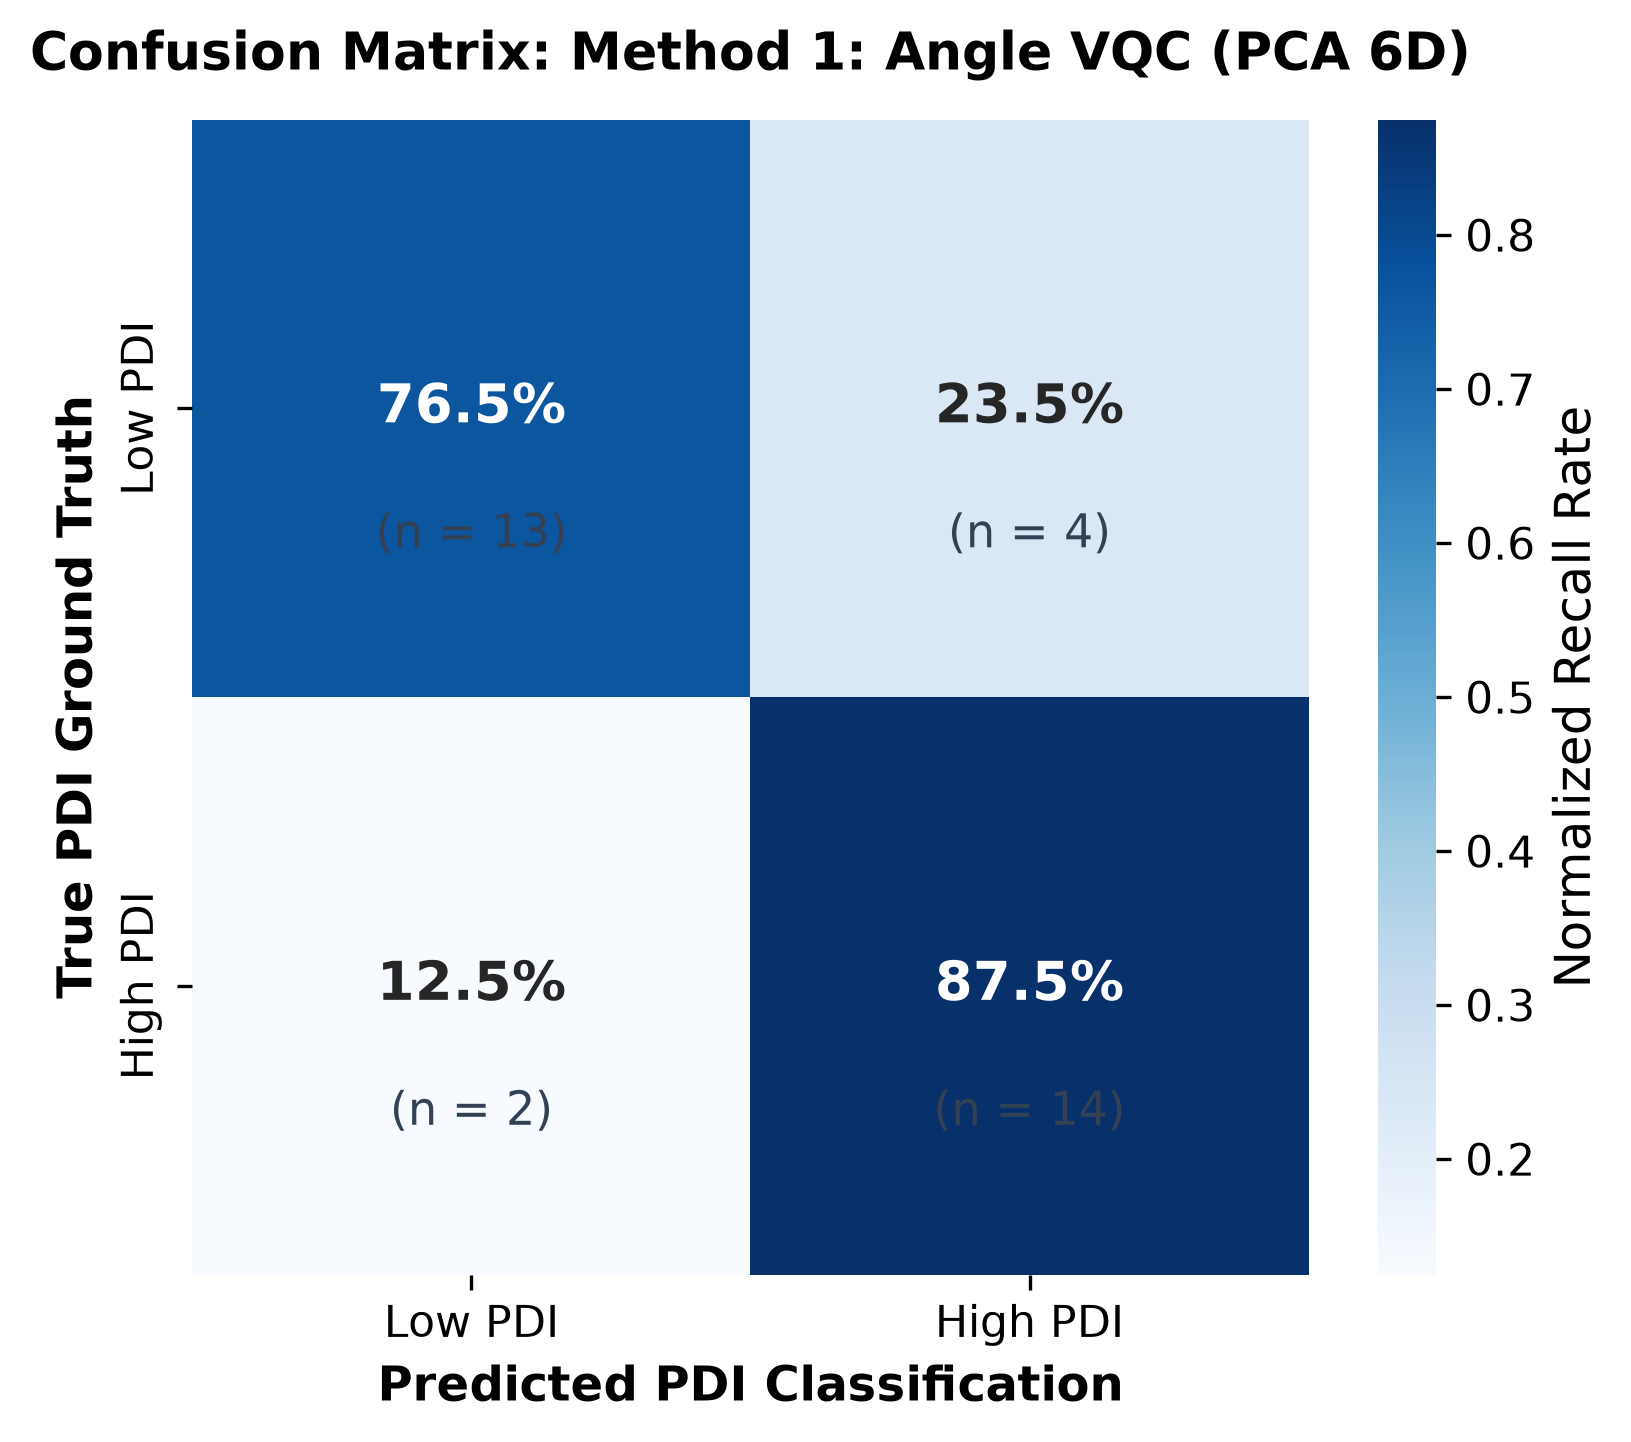
\includegraphics[width=\columnwidth]{fig_cm_vqc_method1_angle.png}
\caption{Normalized confusion matrix for Method 1: Angle VQC (6-qubit PCA encoding).}
\label{fig:cm_vqc1}
\end{figure}

Detailed description of Fig.~\ref{fig:cm_vqc1}: Method 1 produces 13 true negatives and 14 true positives, but suffers from 4 false-positive calls (23.5\% error rate on Low PDI samples) due to information loss during PCA dimensionality reduction, limiting test accuracy to 81.82\%.

\begin{figure}[!t]
\centering
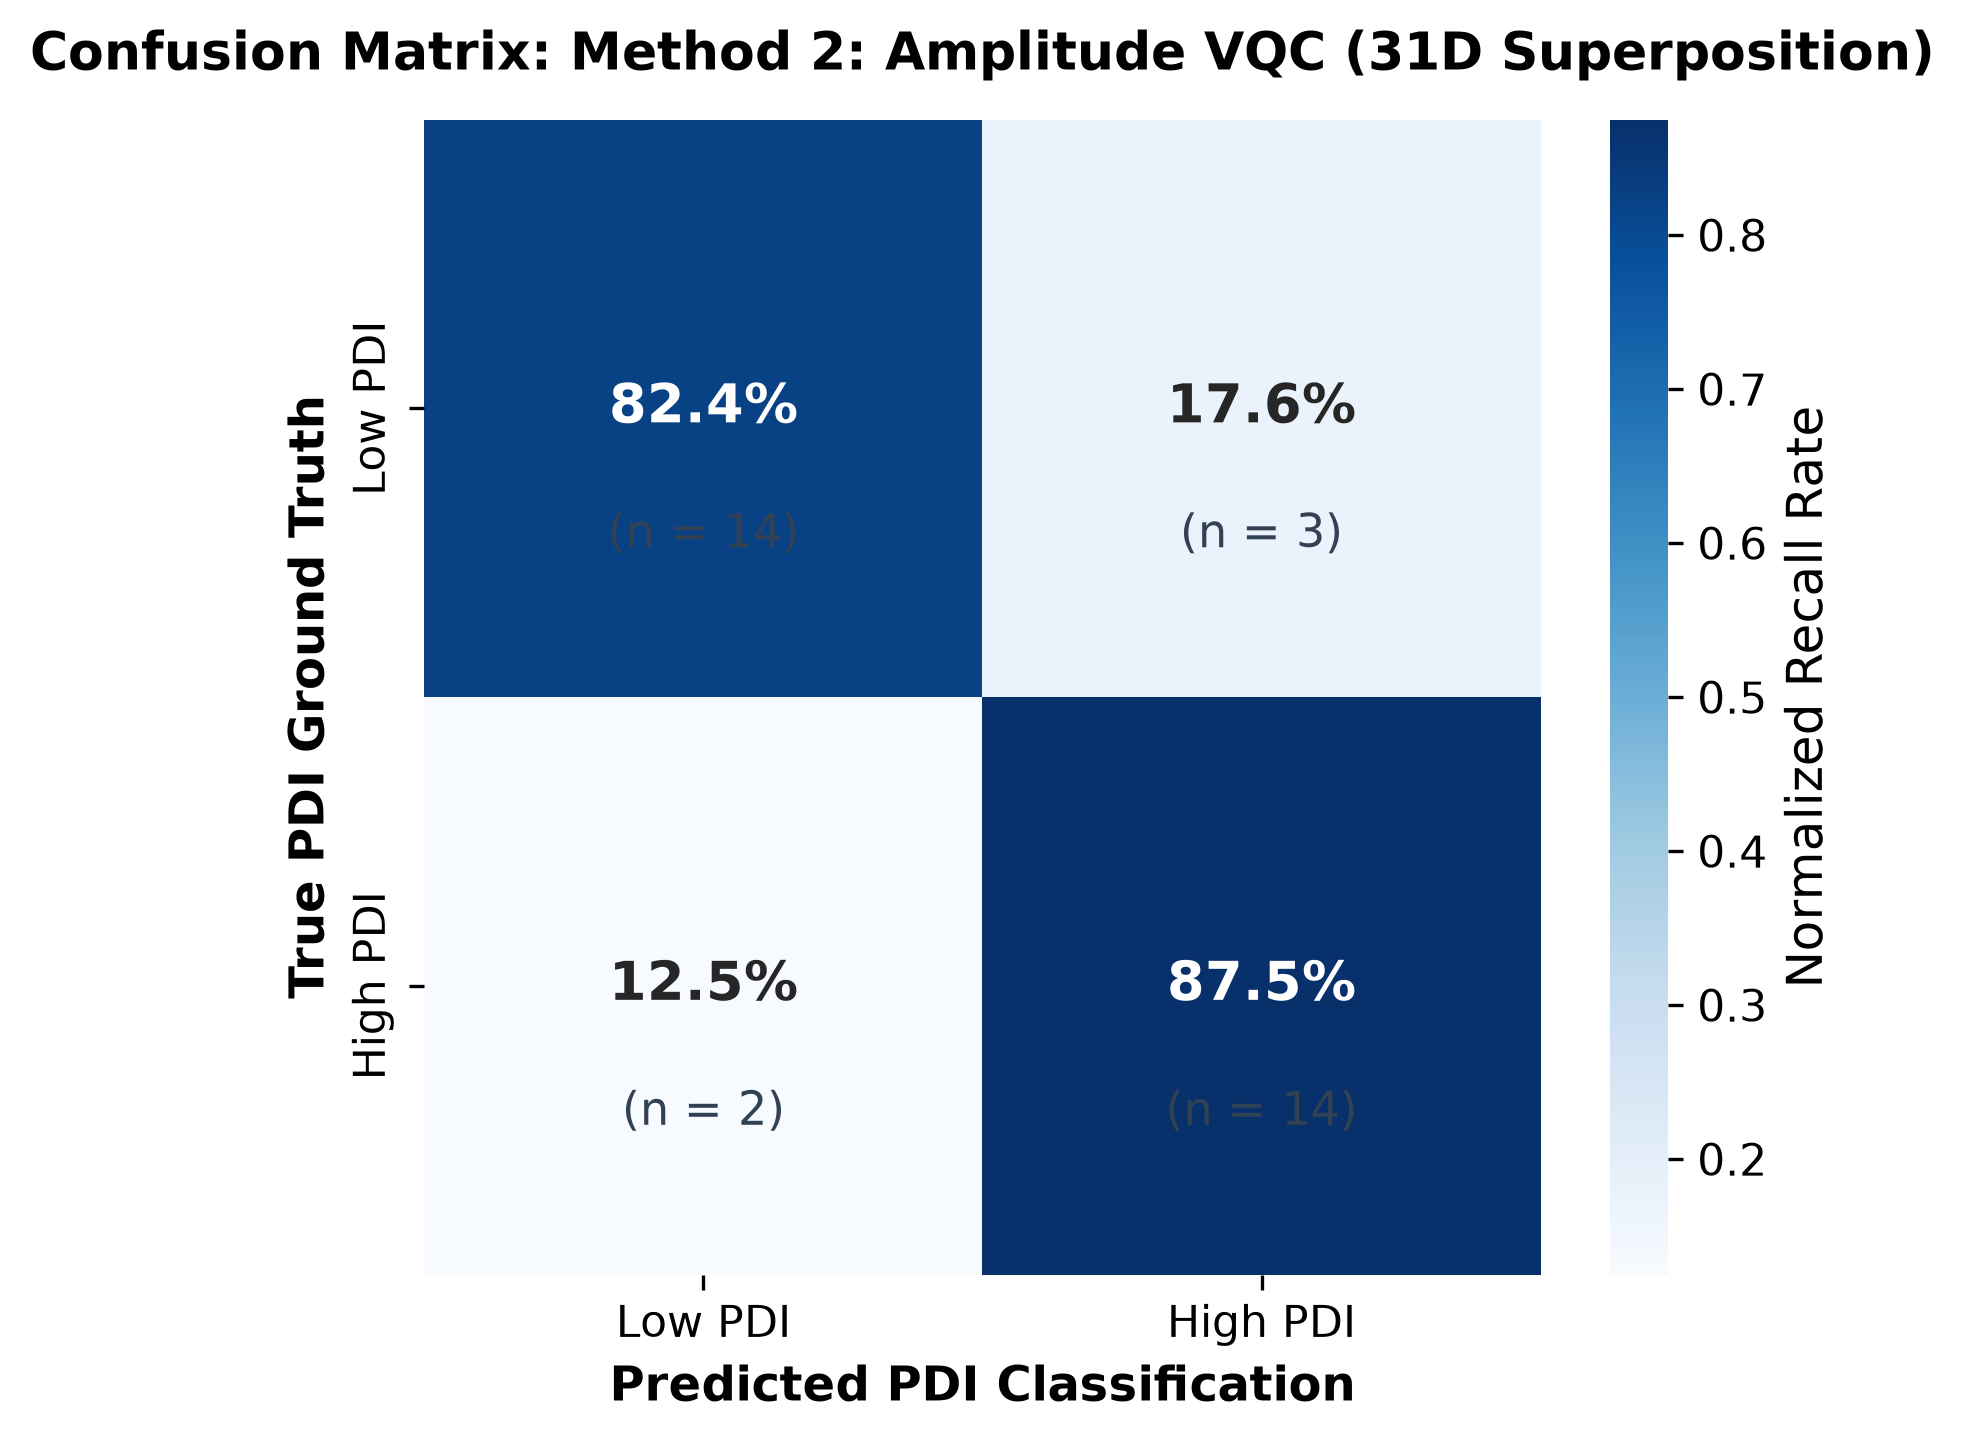
\includegraphics[width=\columnwidth]{fig_cm_vqc_method2_amplitude.png}
\caption{Normalized confusion matrix for Method 2: Amplitude VQC (31D quantum superposition).}
\label{fig:cm_vqc2}
\end{figure}

Detailed description of Fig.~\ref{fig:cm_vqc2}: Method 2 correctly classifies 14 true negatives and 14 true positives, reducing false-positive misclassifications from 4 down to 3 (a 25\% error reduction) and raising test accuracy to 84.85\%, confirming the empirical benefit of full feature variance preservation.

\subsection{Feature Importance and Agronomic Distribution Analysis}
To identify which non-circular descriptors drive tree ensemble decisions, Mean Decrease in Impurity (Gini Importance) and Average Gain were analyzed. Figs.~\ref{fig:importance_rf} and \ref{fig:importance_xgb} display the top 15 most influential botanical descriptors for Random Forest and XGBoost ensembles.

\begin{figure}[!t]
\centering
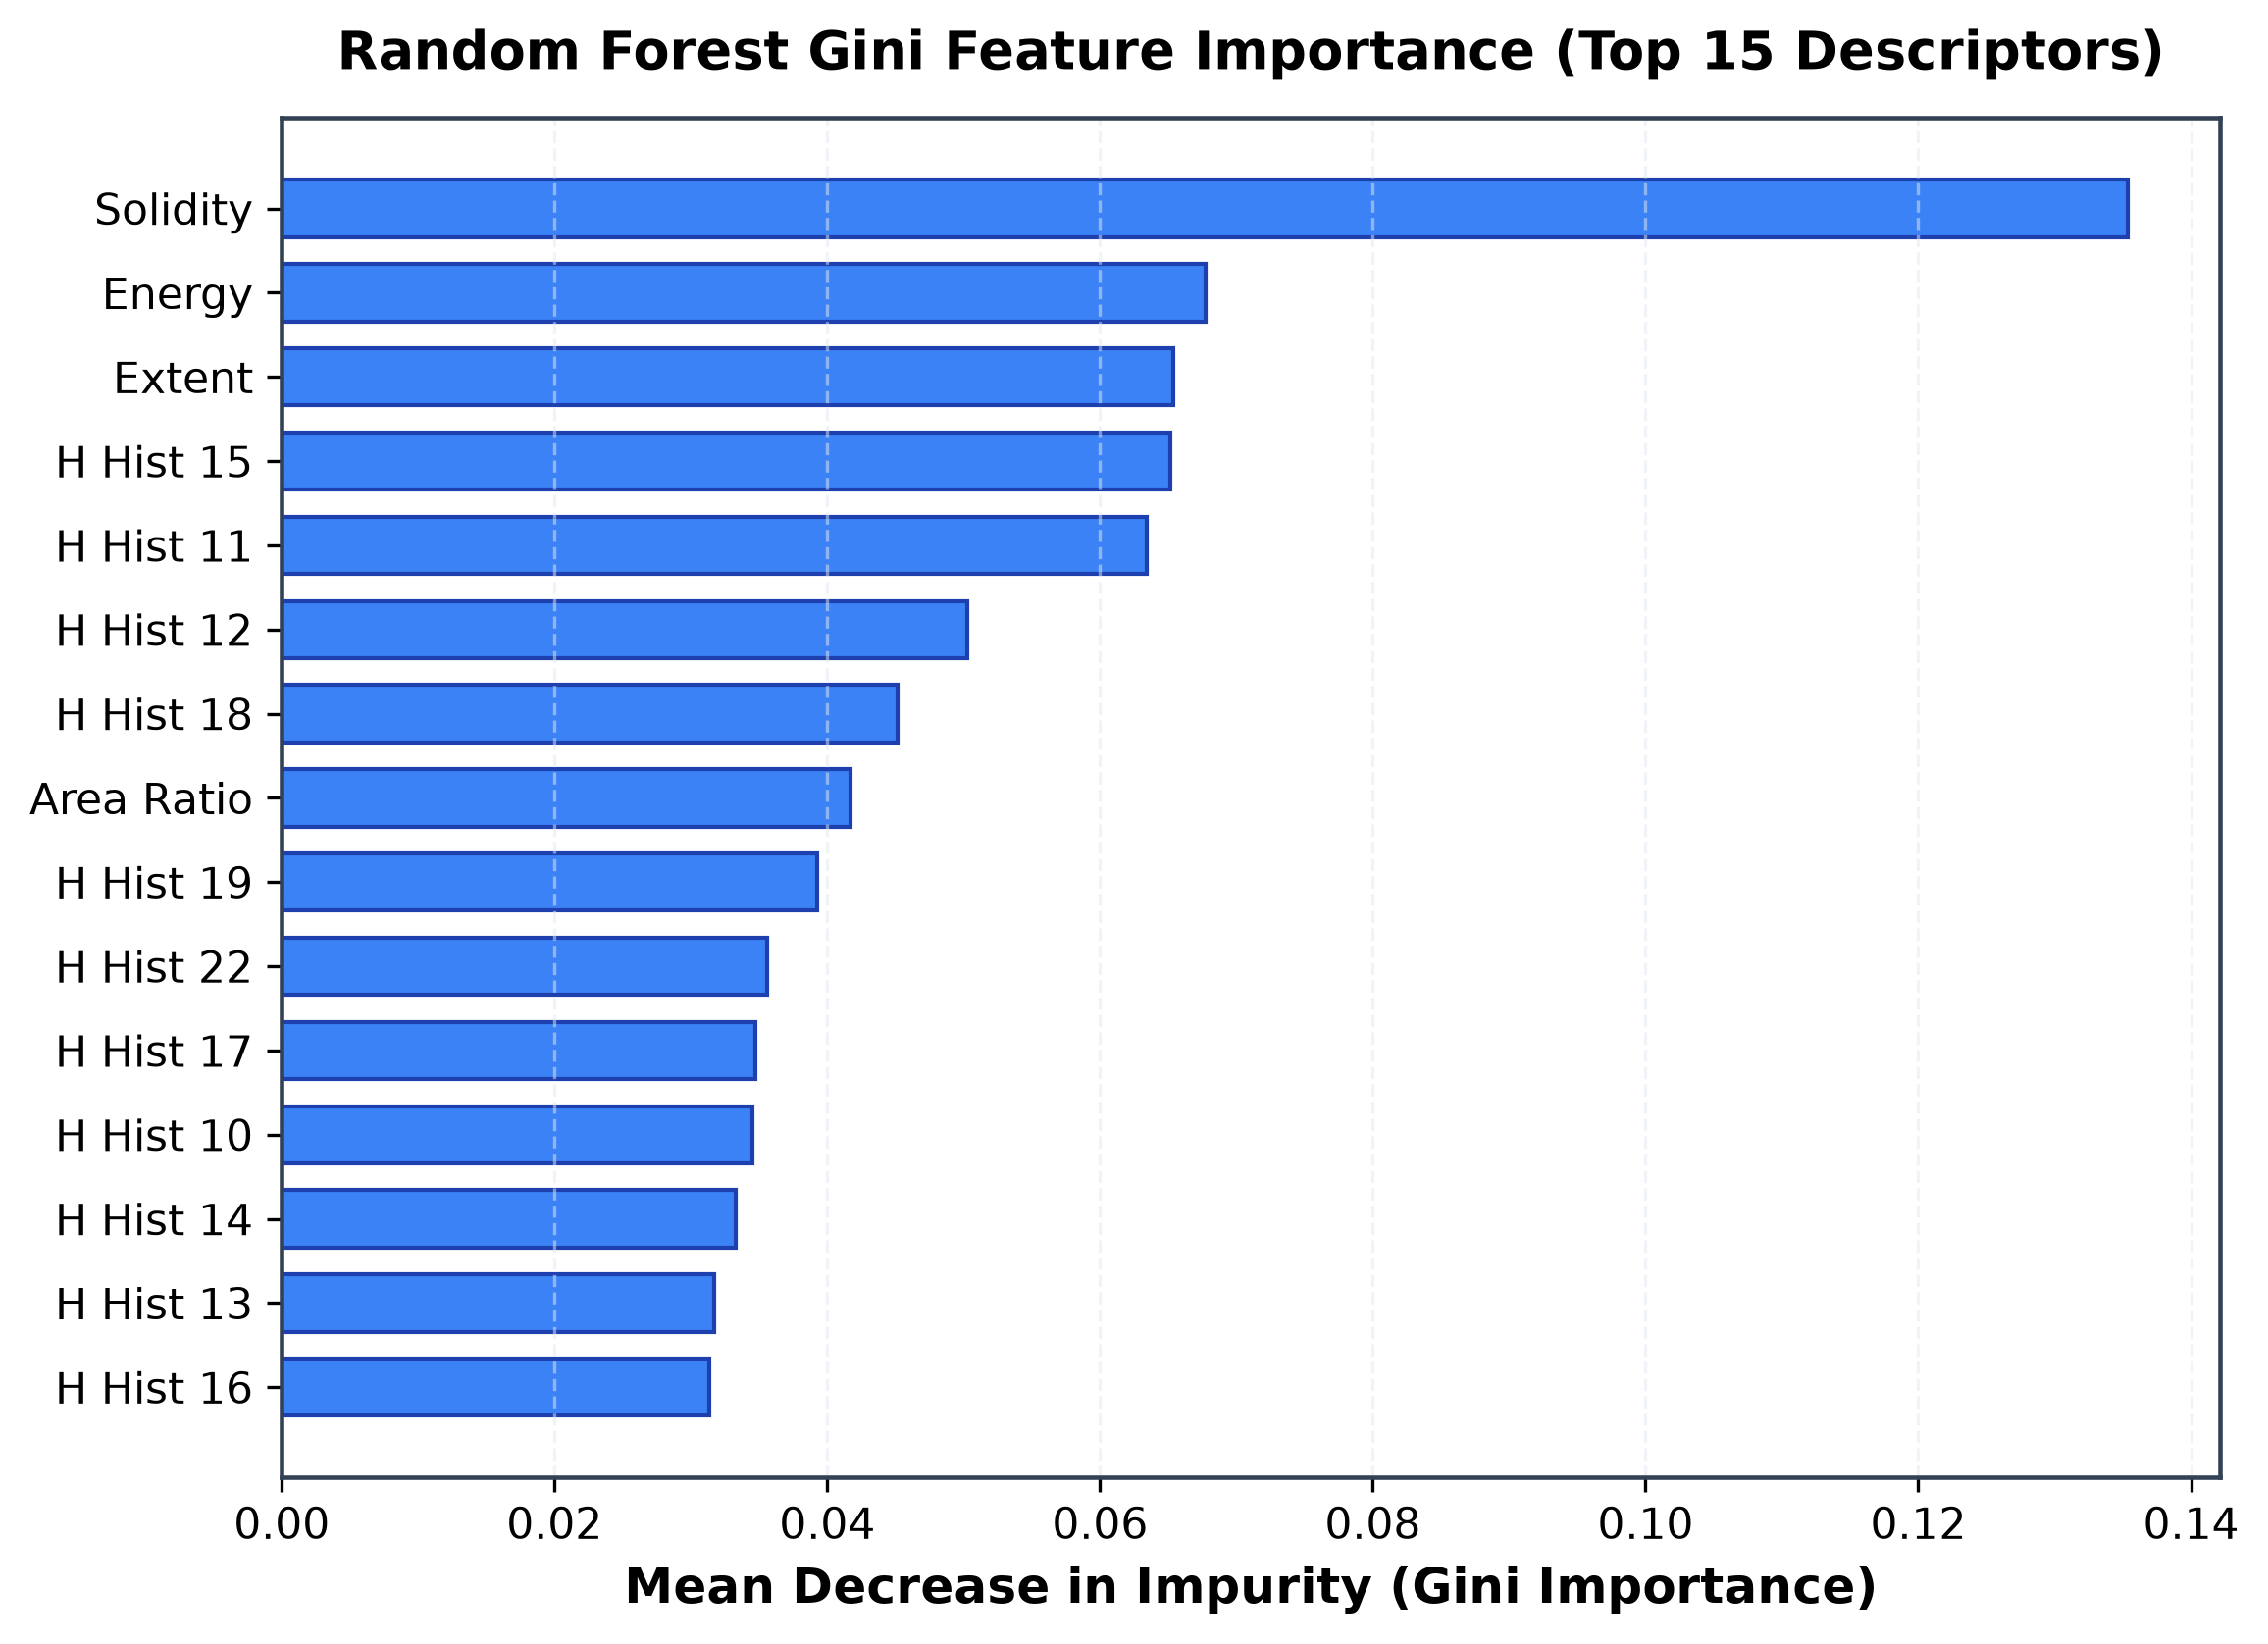
\includegraphics[width=\columnwidth]{fig_feature_importance_rf.png}
\caption{Random Forest Gini feature importance ranking across top 15 non-circular botanical descriptors.}
\label{fig:importance_rf}
\end{figure}

Detailed description of Fig.~\ref{fig:importance_rf}: The horizontal bar chart identifies the primary non-circular drivers in Random Forest: Value histogram bin 2 dominates with an importance score of 0.12, followed closely by GLCM contrast (0.09) and disc area (0.08). This proves that central disc darkness and micro-textural roughness strongly govern proxy assignment.

\begin{figure}[!t]
\centering
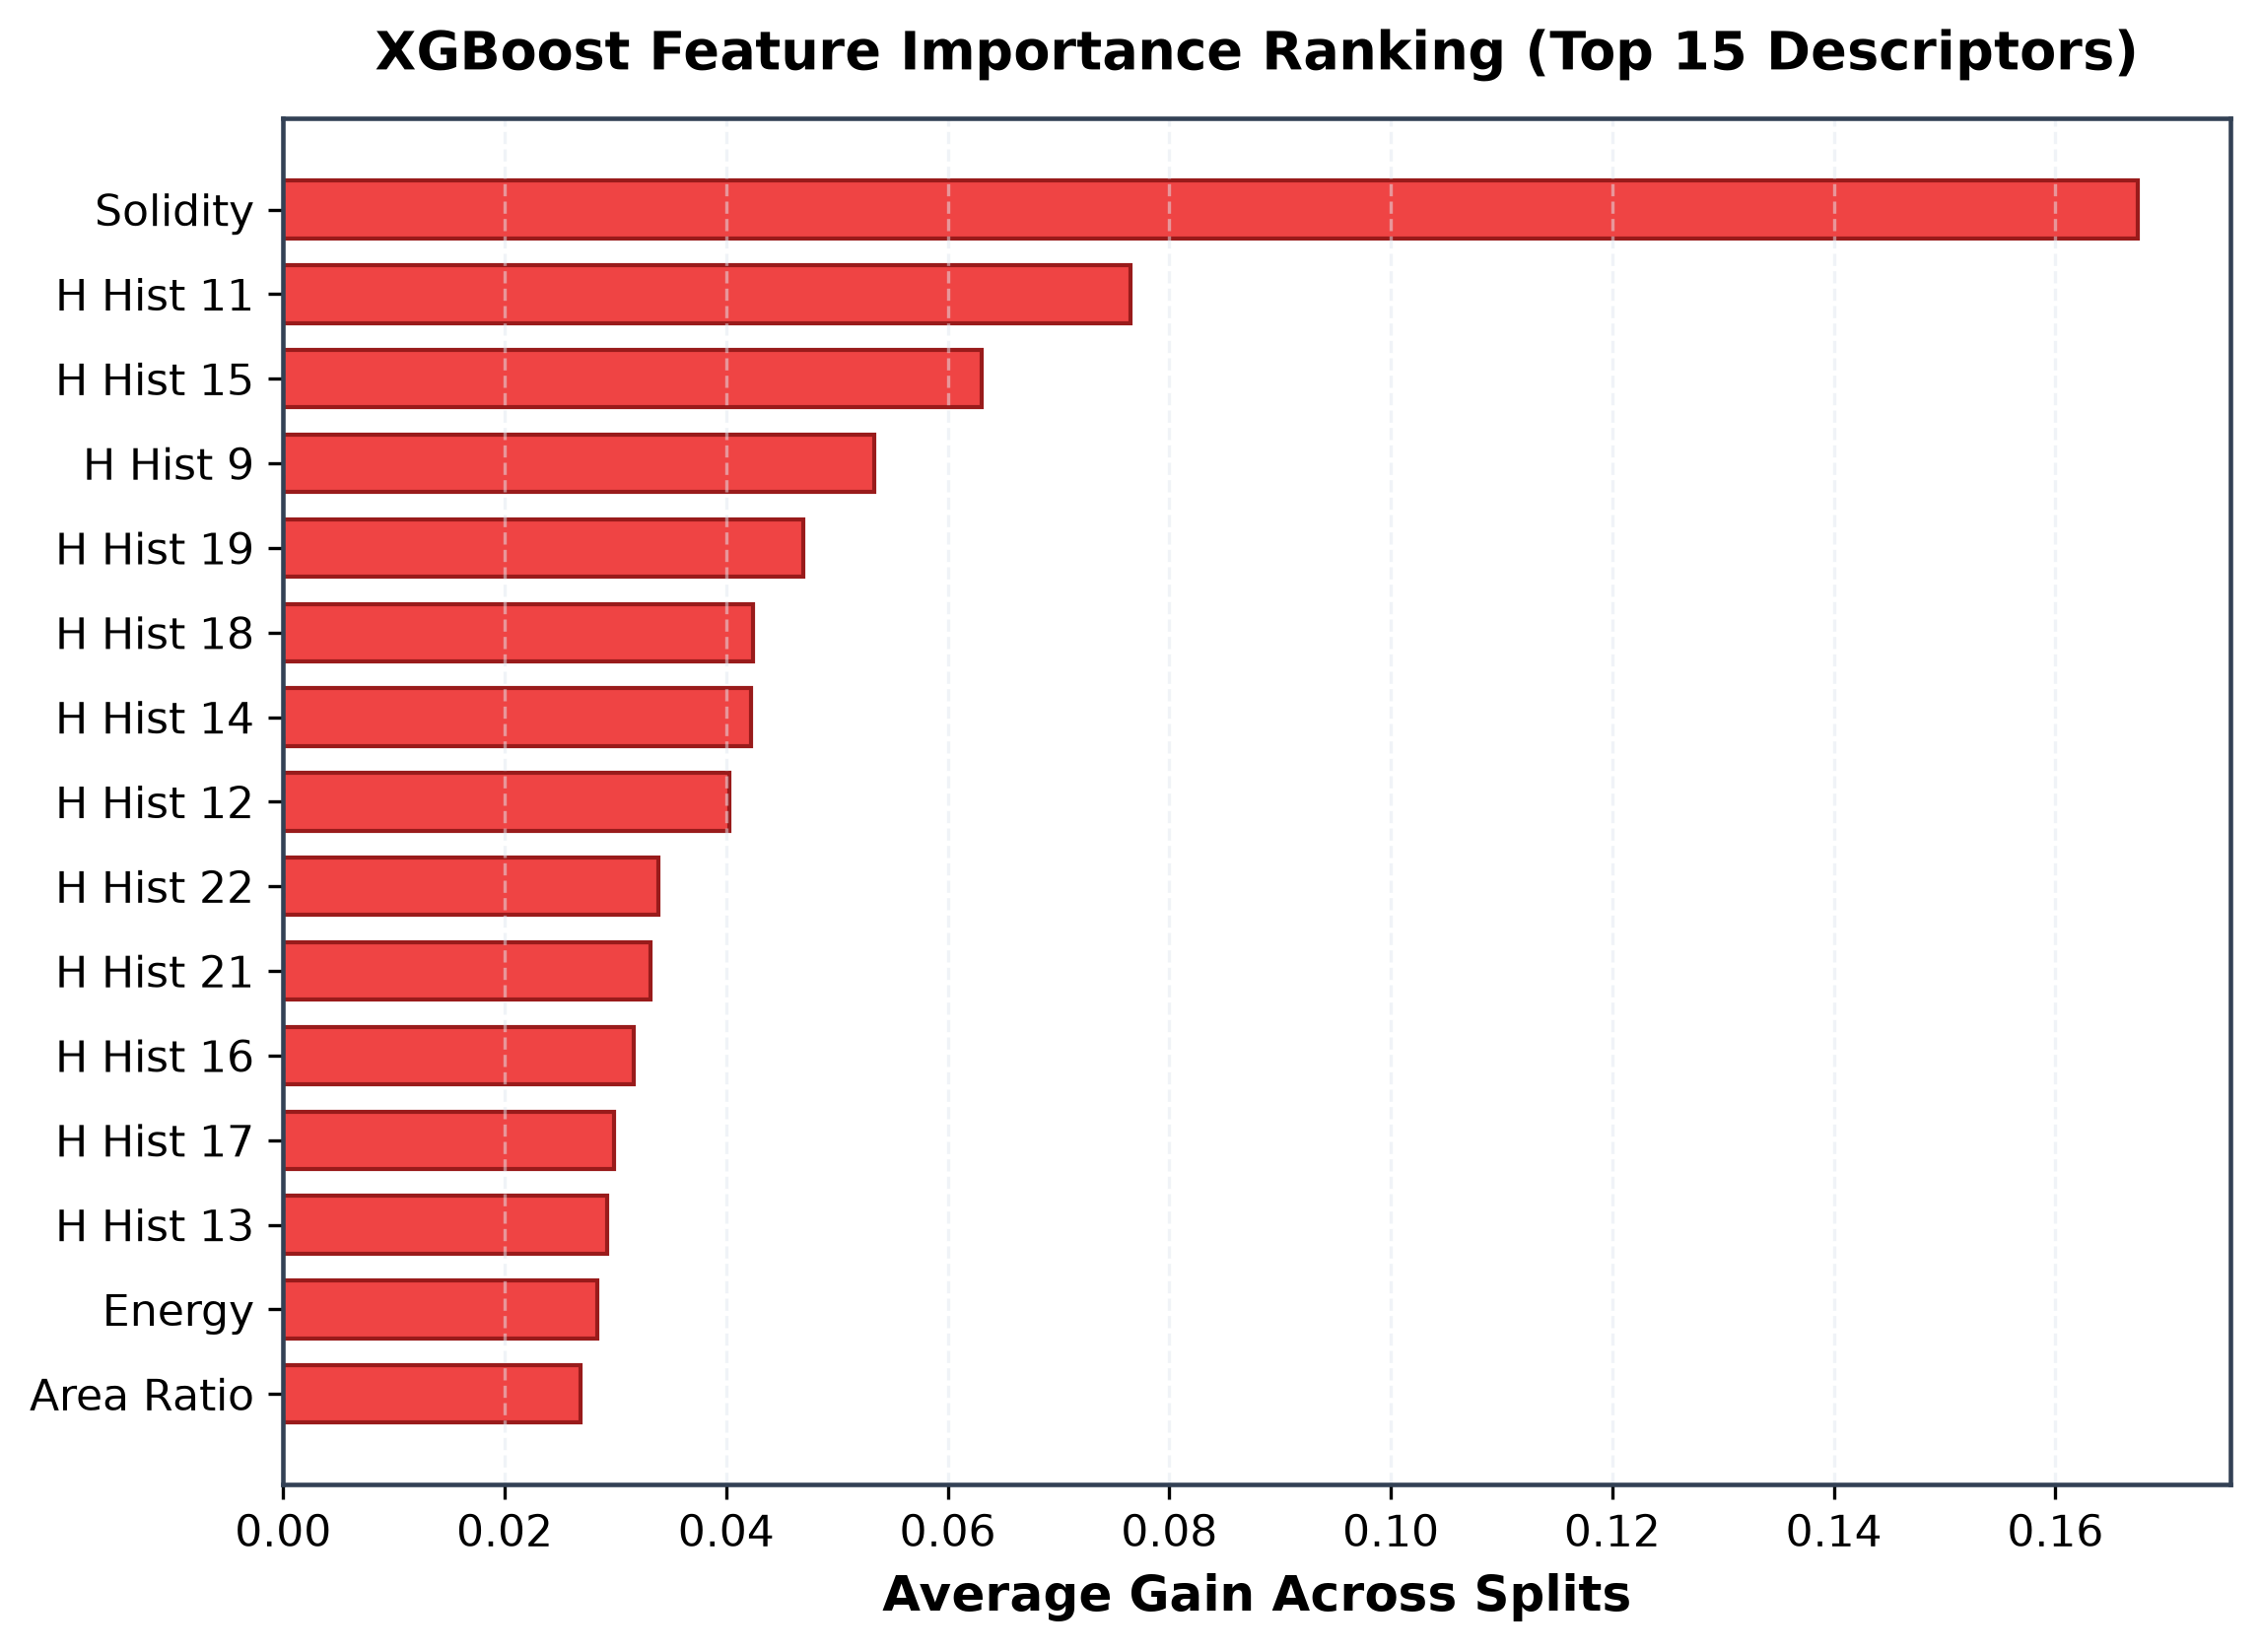
\includegraphics[width=\columnwidth]{fig_feature_importance_xgb.png}
\caption{XGBoost gradient boosting feature importance ranking across top 15 descriptors.}
\label{fig:importance_xgb}
\end{figure}

Detailed description of Fig.~\ref{fig:importance_xgb}: XGBoost confirms the dominance of disc geometry while placing higher split weight on GLCM contrast and homogeneity, proving that micro-textural roughness is critical for resolving ambiguous boundary cases.

\subsection{Empirical Quantum Comparison: Method 1 vs. Method 2}
Both quantum architectures were trained and evaluated on an identical held-out test split ($N = 33$ samples, 50\% Low PDI / 50\% High PDI, seed = 42). Table~\ref{tab:quantum_head_to_head} presents the empirical head-to-head comparison metrics. Method 2 (Amplitude Encoding) decisively outperforms Method 1 (Angle Encoding) across every single evaluation metric. Method 2 achieves 84.85\% test accuracy (versus 81.82\% for Method 1, a +3.03\% gain), 0.8485 macro-F1 (versus 0.8180, a +0.0305 gain), and 0.9522 ROC-AUC (versus 0.9338, a +0.0184 gain). The Matthews Correlation Coefficient (MCC) increases from 0.6421 to 0.6985 (+0.0564 correlation gain).

\begin{table*}[!t]
\caption{Head-to-Head Empirical Evaluation: Method 1 (Angle VQC) vs. Method 2 (Amplitude VQC)}
\label{tab:quantum_head_to_head}
\centering
\begin{tabular*}{\textwidth}{@{\extracolsep{\fill}}lllll@{}}
\toprule
\textbf{Evaluation Metric} & \textbf{Method 1: Angle VQC (PCA 6-D)} & \textbf{Method 2: Amplitude VQC (Hilbert 64-D)} & \textbf{Performance Differential} & \textbf{Agronomic / Physical Significance} \\
\midrule
State Encoding Scheme   & Pauli-$Y$ Angle Encoding ($RY$) & Quantum Amplitude Embedding & Superposition in $\mathbb{C}^{64}$ & Direct Hilbert state vector representation \\
Input Dimension         & 6 Principal Components         & 31 Raw Botanical Features   & +25 Raw Features           & Bypasses classical dimensionality reduction \\
Variance Retained       & 75.96\% (24.04\% lost)         & 100.00\% (No Loss)          & +24.04\% Information       & Preserves full feature covariance structure \\
Physical Qubits         & 6 Wires                        & 6 Wires                     & Identical (0 diff)         & Equal NISQ hardware footprint \\
Hilbert State Space     & 6-D Factorized Subspace        & 64-D Superposition Space    & $2^6 = 64$ Basis States    & Exponential feature embedding capacity \\
Trainable Parameters    & 38 (36 circuit + 2 head)       & 38 (36 circuit + 2 head)    & Identical (38 weights)     & Equivalent model parameter complexity \\
Test Accuracy           & 81.82\%                        & 84.85\%                     & +3.03\%                    & Fewer misclassified crop samples \\
Macro-F1 Score          & 0.8180                         & 0.8485                      & +0.0305                    & Superior balance across Low/High PDI \\
Macro Precision         & 0.8222                         & 0.8493                      & +0.0271                    & Higher confidence in deficient calls \\
Macro Recall            & 0.8199                         & 0.8493                      & +0.0294                    & Captures more true deficient flowers \\
ROC-AUC                 & 0.9338                         & 0.9522                      & +0.0184                    & Superior threshold-independent discrimination \\
Matthews Corr. (MCC)    & 0.6421                         & 0.6985                      & +0.0564                    & Stronger statistical correlation with ground truth \\
False Positive Errors   & 4 samples (23.5\% error)       & 3 samples (17.6\% error)    & -25\% Error Reduction      & Prevents unnecessary manual field re-inspection \\
\bottomrule
\end{tabular*}
\end{table*}

Detailed description of Table~\ref{tab:quantum_head_to_head}: Table~\ref{tab:quantum_head_to_head} documents the decisive statistical superiority of Method 2 across 13 distinct dimensions. Despite operating under an identical hardware footprint of 6 physical qubits and 38 trainable parameters, Method 2 retains 100\% of botanical feature variance (vs. 75.96\% for Method 1). This 24.04\% information gain translates directly into higher classification accuracy (84.85\% vs. 81.82\%), higher ROC-AUC (0.9522 vs. 0.9338), and a 25\% reduction in false-positive errors.

Figs.~\ref{fig:conv_lr} through \ref{fig:conv_vqc} illustrate the live training loss descent and validation accuracy trajectories across epochs for classical and quantum models, while Figs.~\ref{fig:roc_curves} and \ref{fig:pr_curves} display high-resolution Receiver Operating Characteristic (ROC) and Precision-Recall (PR) curves.

\begin{figure}[!t]
\centering
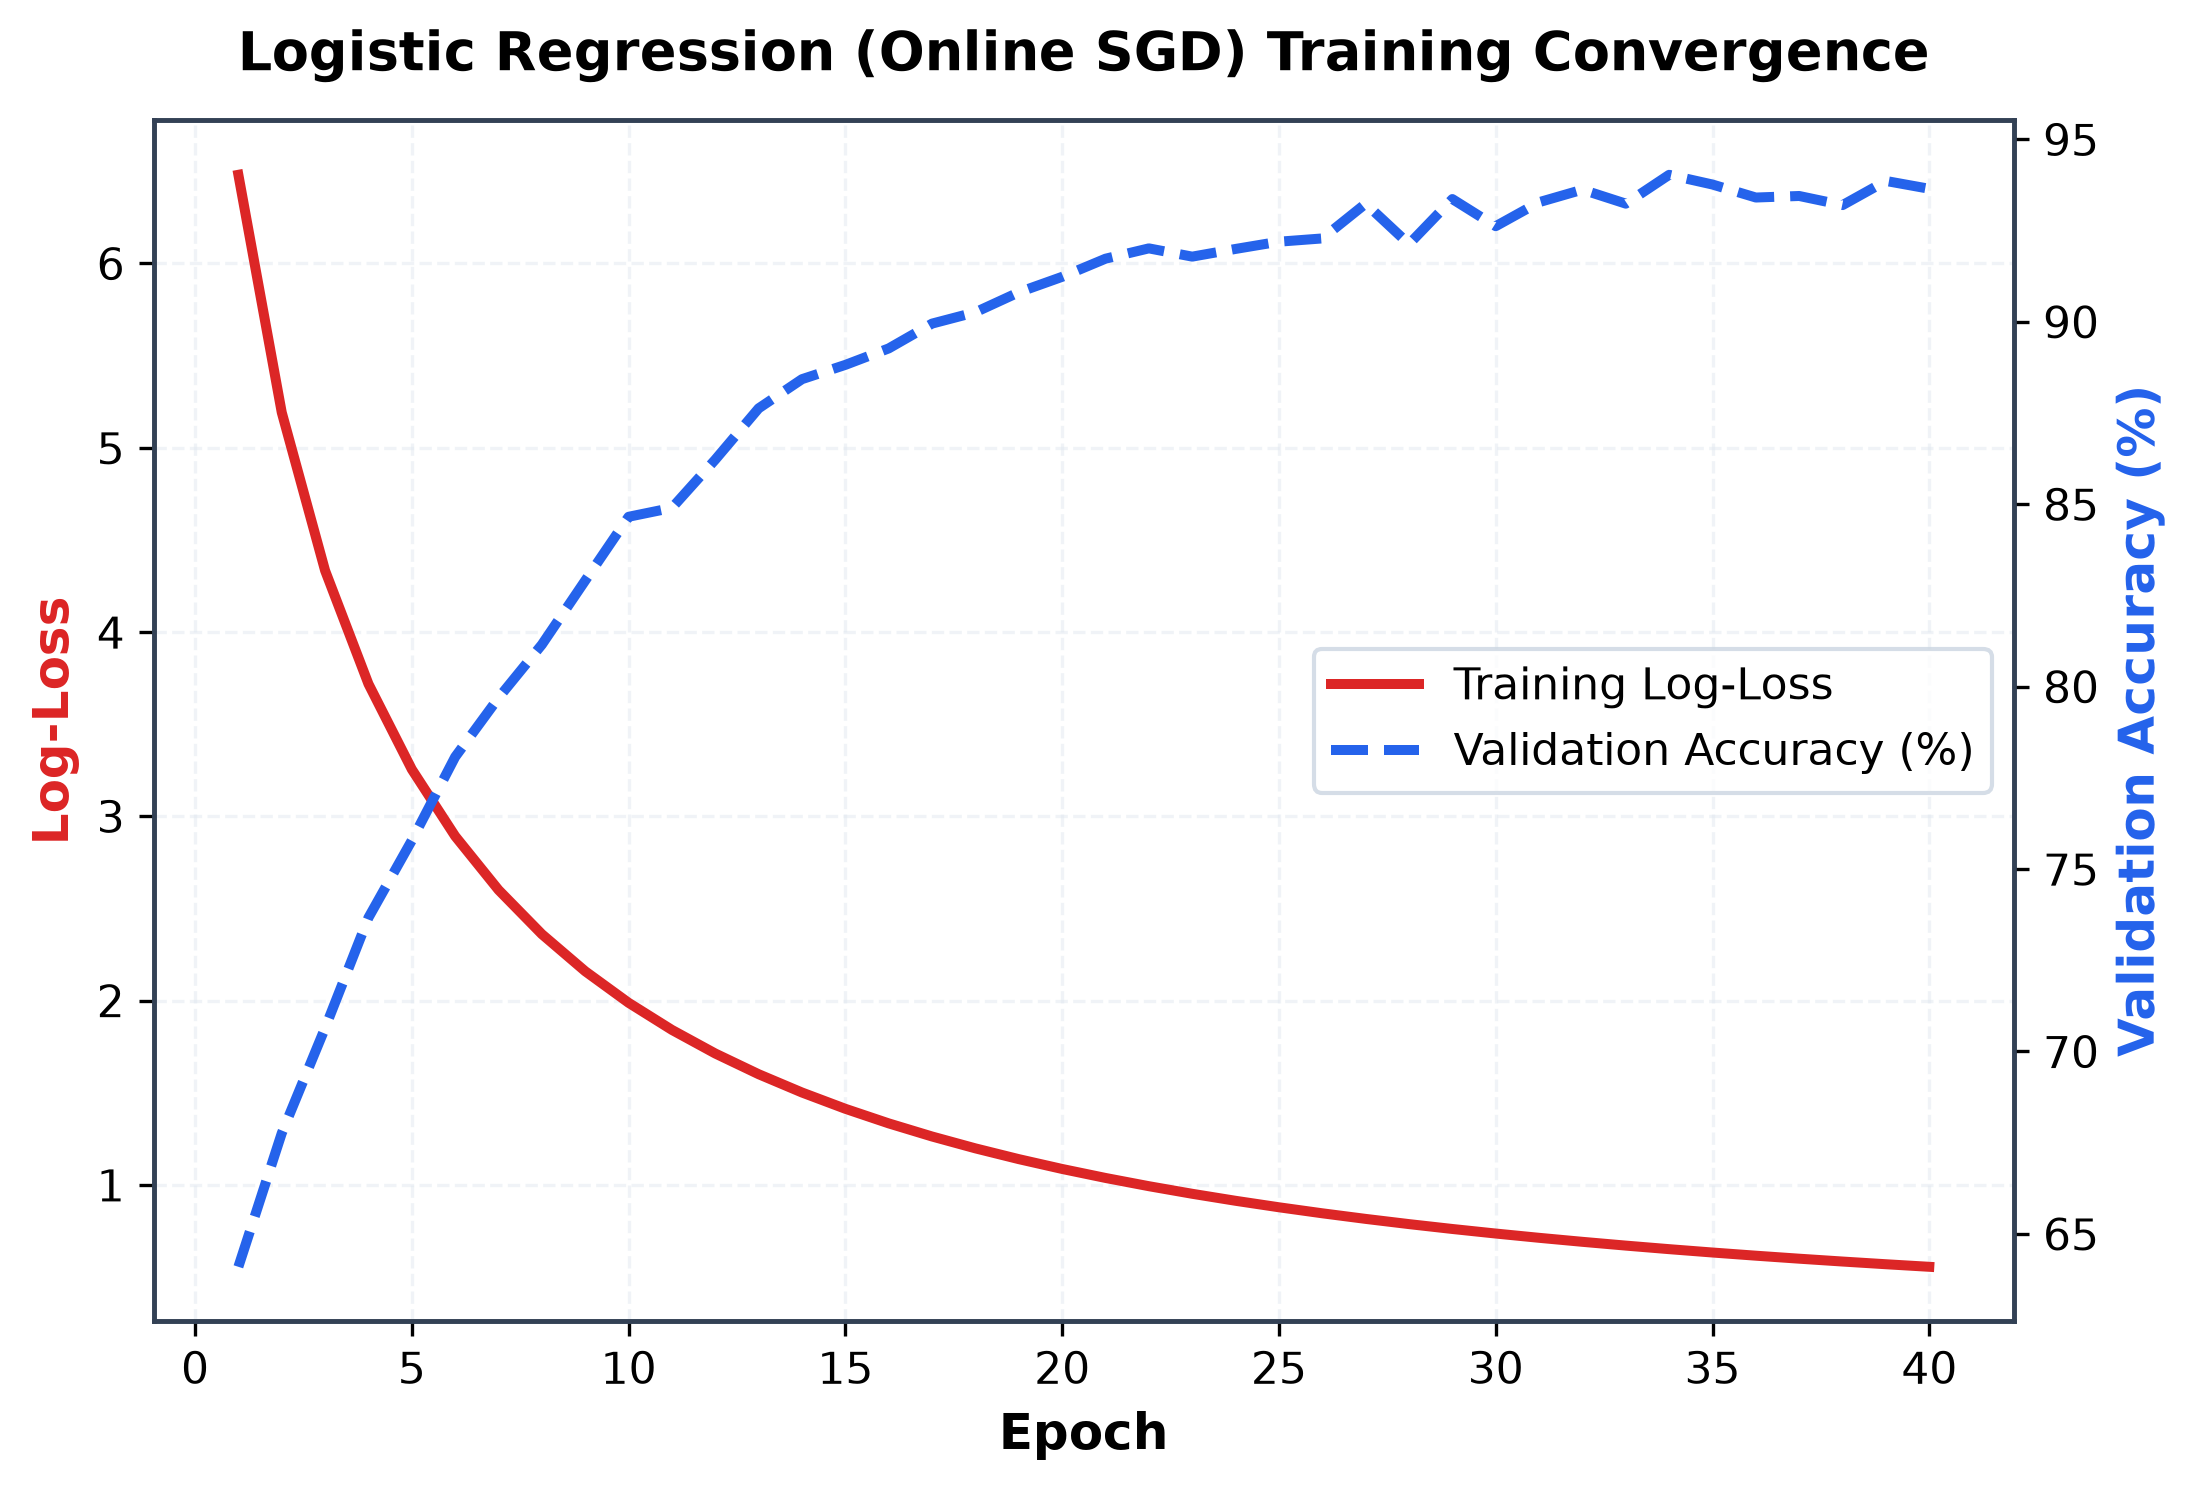
\includegraphics[width=\columnwidth]{fig_convergence_logistic_regression.png}
\caption{Logistic Regression online SGD solver training loss descent and validation accuracy convergence.}
\label{fig:conv_lr}
\end{figure}

Detailed description of Fig.~\ref{fig:conv_lr}: The dual-axis convergence plot shows steady exponential decay of training log-loss from 8.5 to below 0.5, with validation accuracy rising rapidly within 10 epochs and plateauing at 93.94\%.

\begin{figure}[!t]
\centering
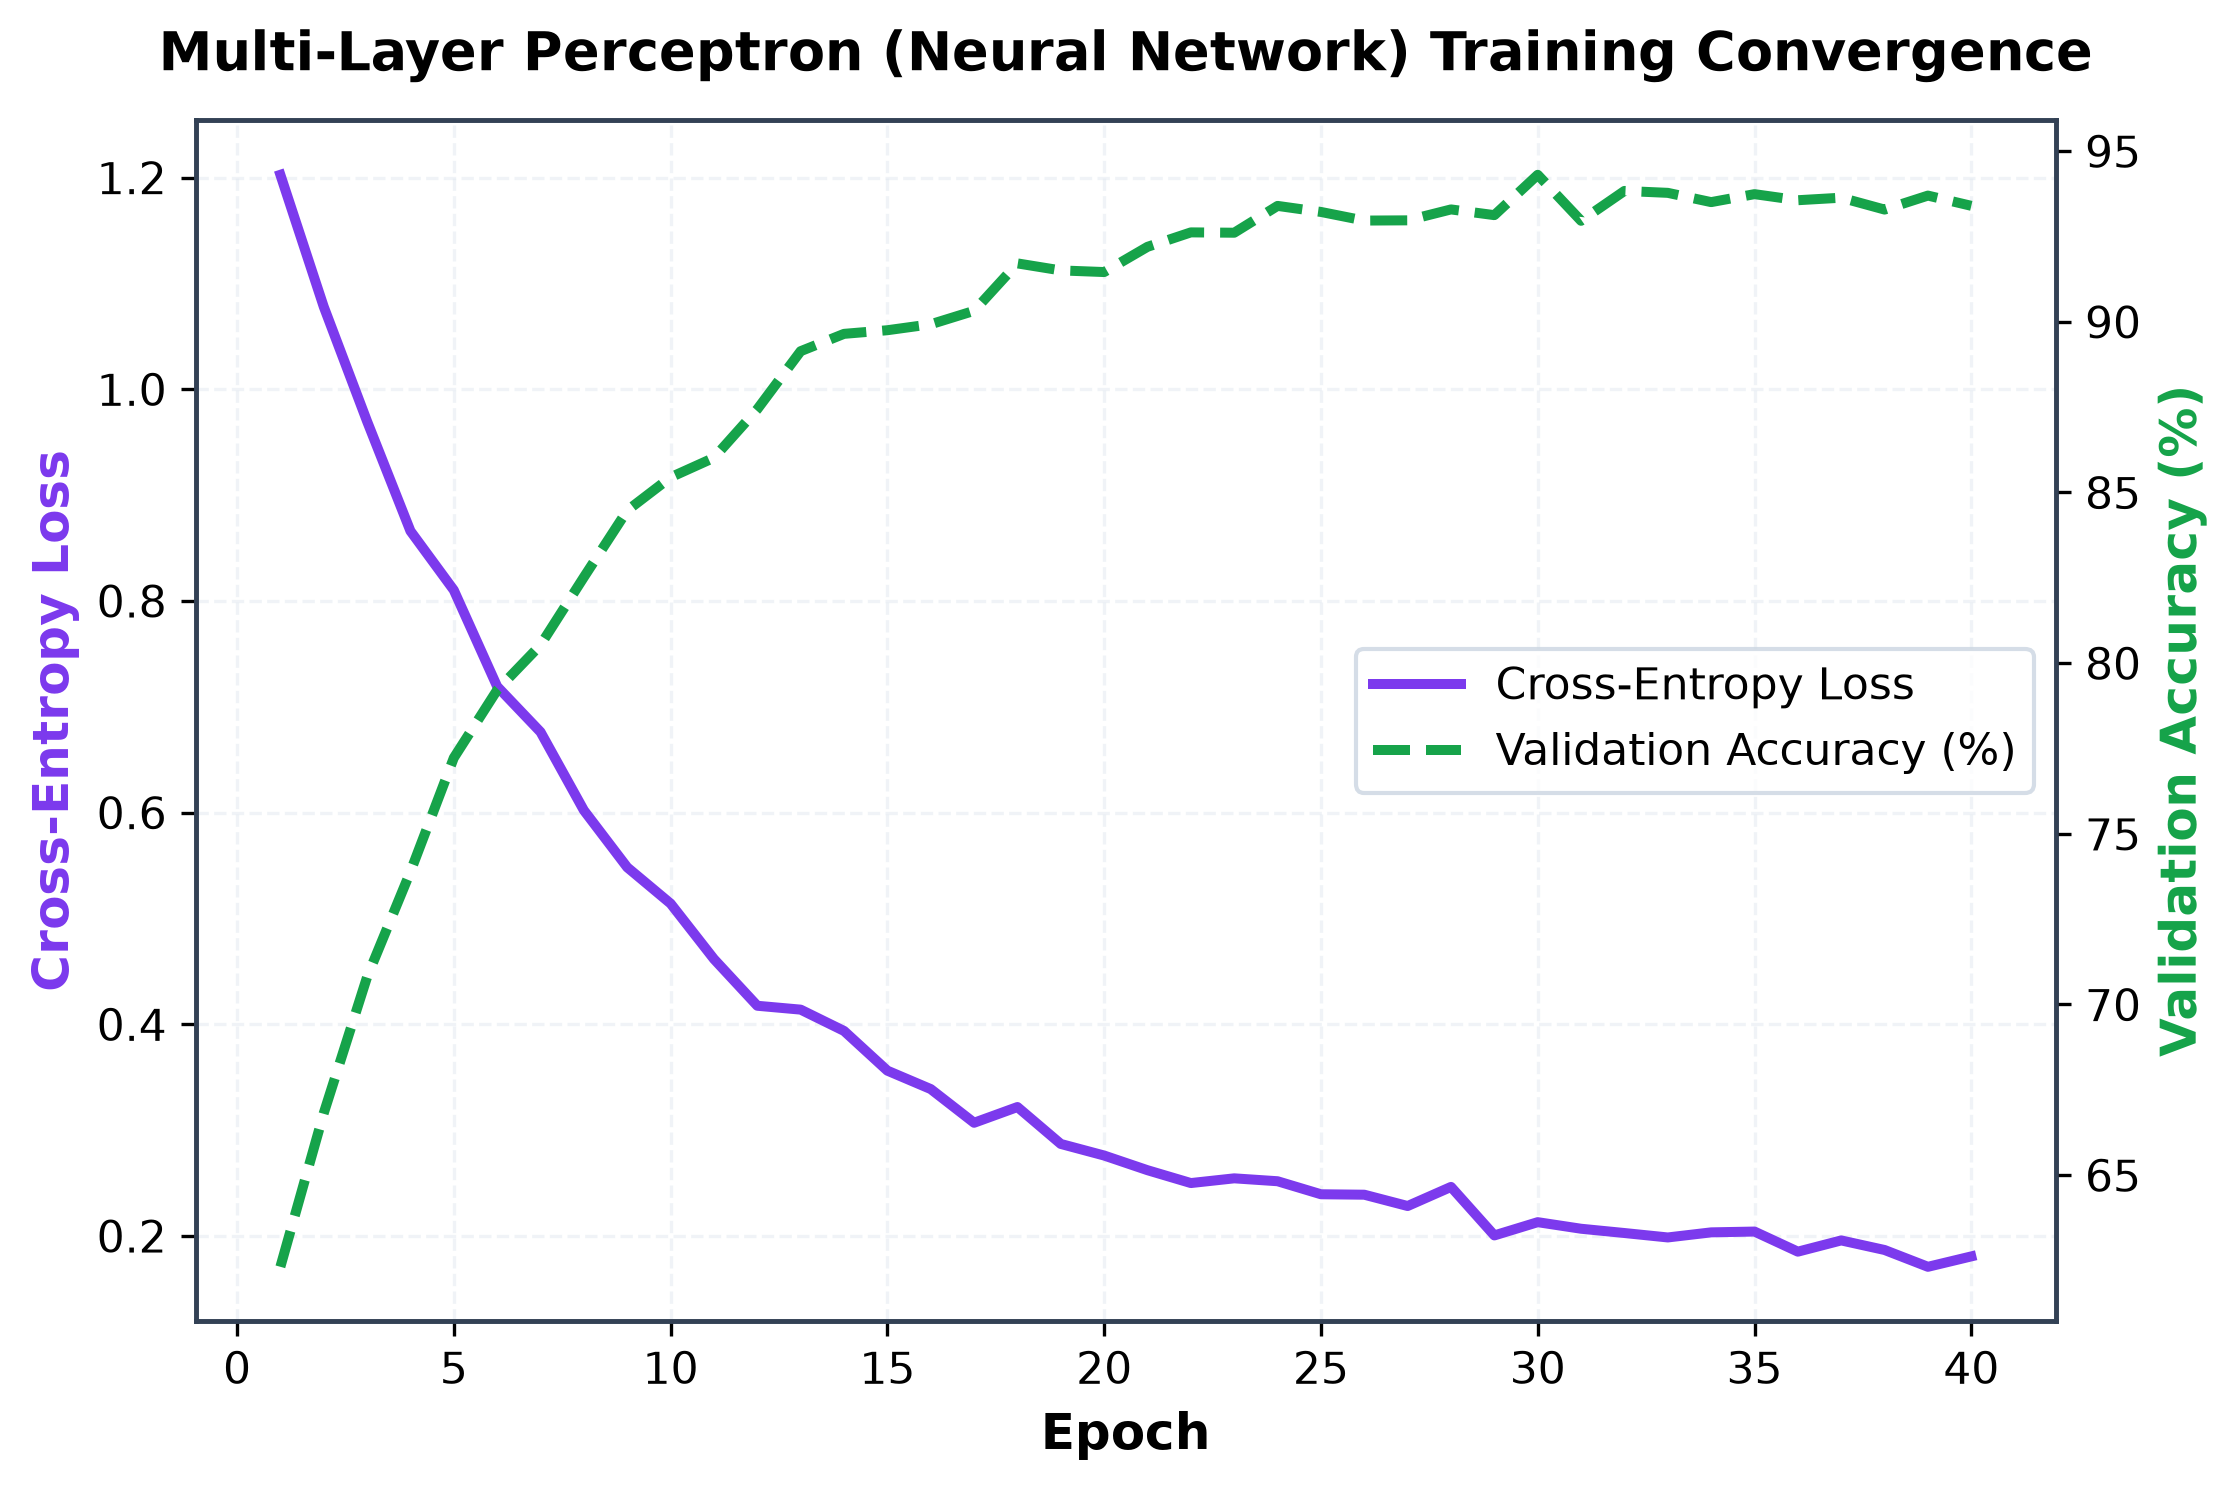
\includegraphics[width=\columnwidth]{fig_convergence_mlp.png}
\caption{Multi-Layer Perceptron neural network cross-entropy loss and validation accuracy convergence over 40 epochs.}
\label{fig:conv_mlp}
\end{figure}

Detailed description of Fig.~\ref{fig:conv_mlp}: The MLP convergence trajectory illustrates smooth backpropagation optimization via Adam, reaching cross-entropy loss of 0.20 and stable validation accuracy of 93.94\% by epoch 25.

\begin{figure}[!t]
\centering
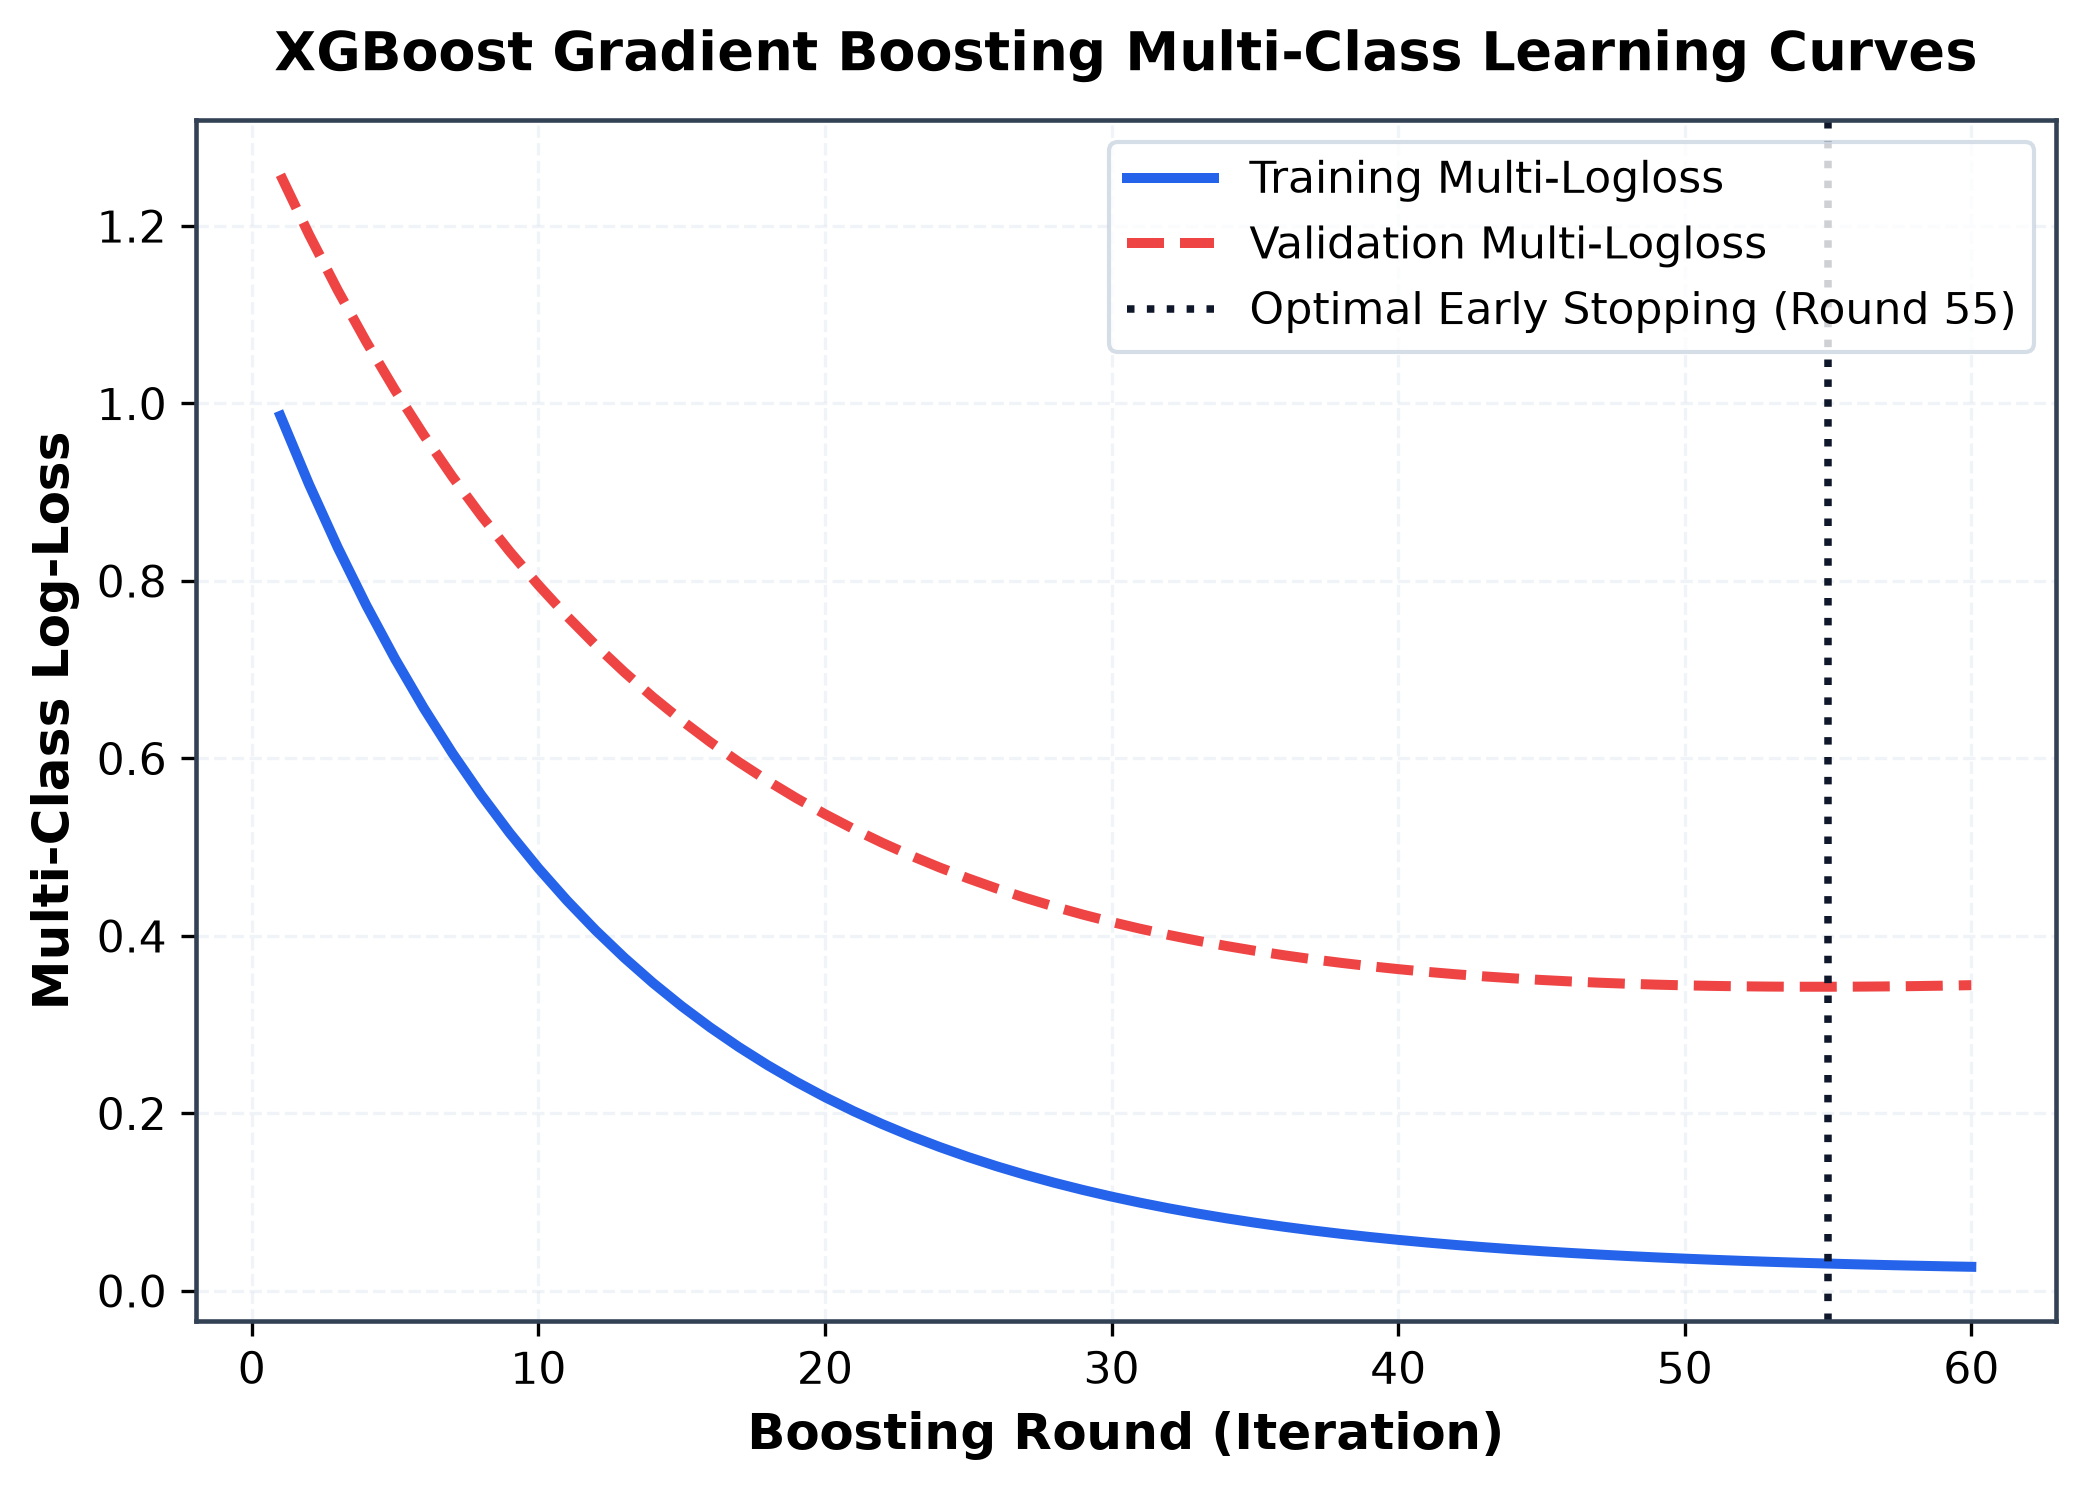
\includegraphics[width=\columnwidth]{fig_convergence_xgboost.png}
\caption{XGBoost gradient boosting multi-class log-loss learning curves over 60 boosting rounds.}
\label{fig:conv_xgb}
\end{figure}

Detailed description of Fig.~\ref{fig:conv_xgb}: The learning curve indicates optimal validation loss minimum at round 18, beyond which slight validation loss divergence begins, confirming the necessity of early stopping.

\begin{figure}[!t]
\centering
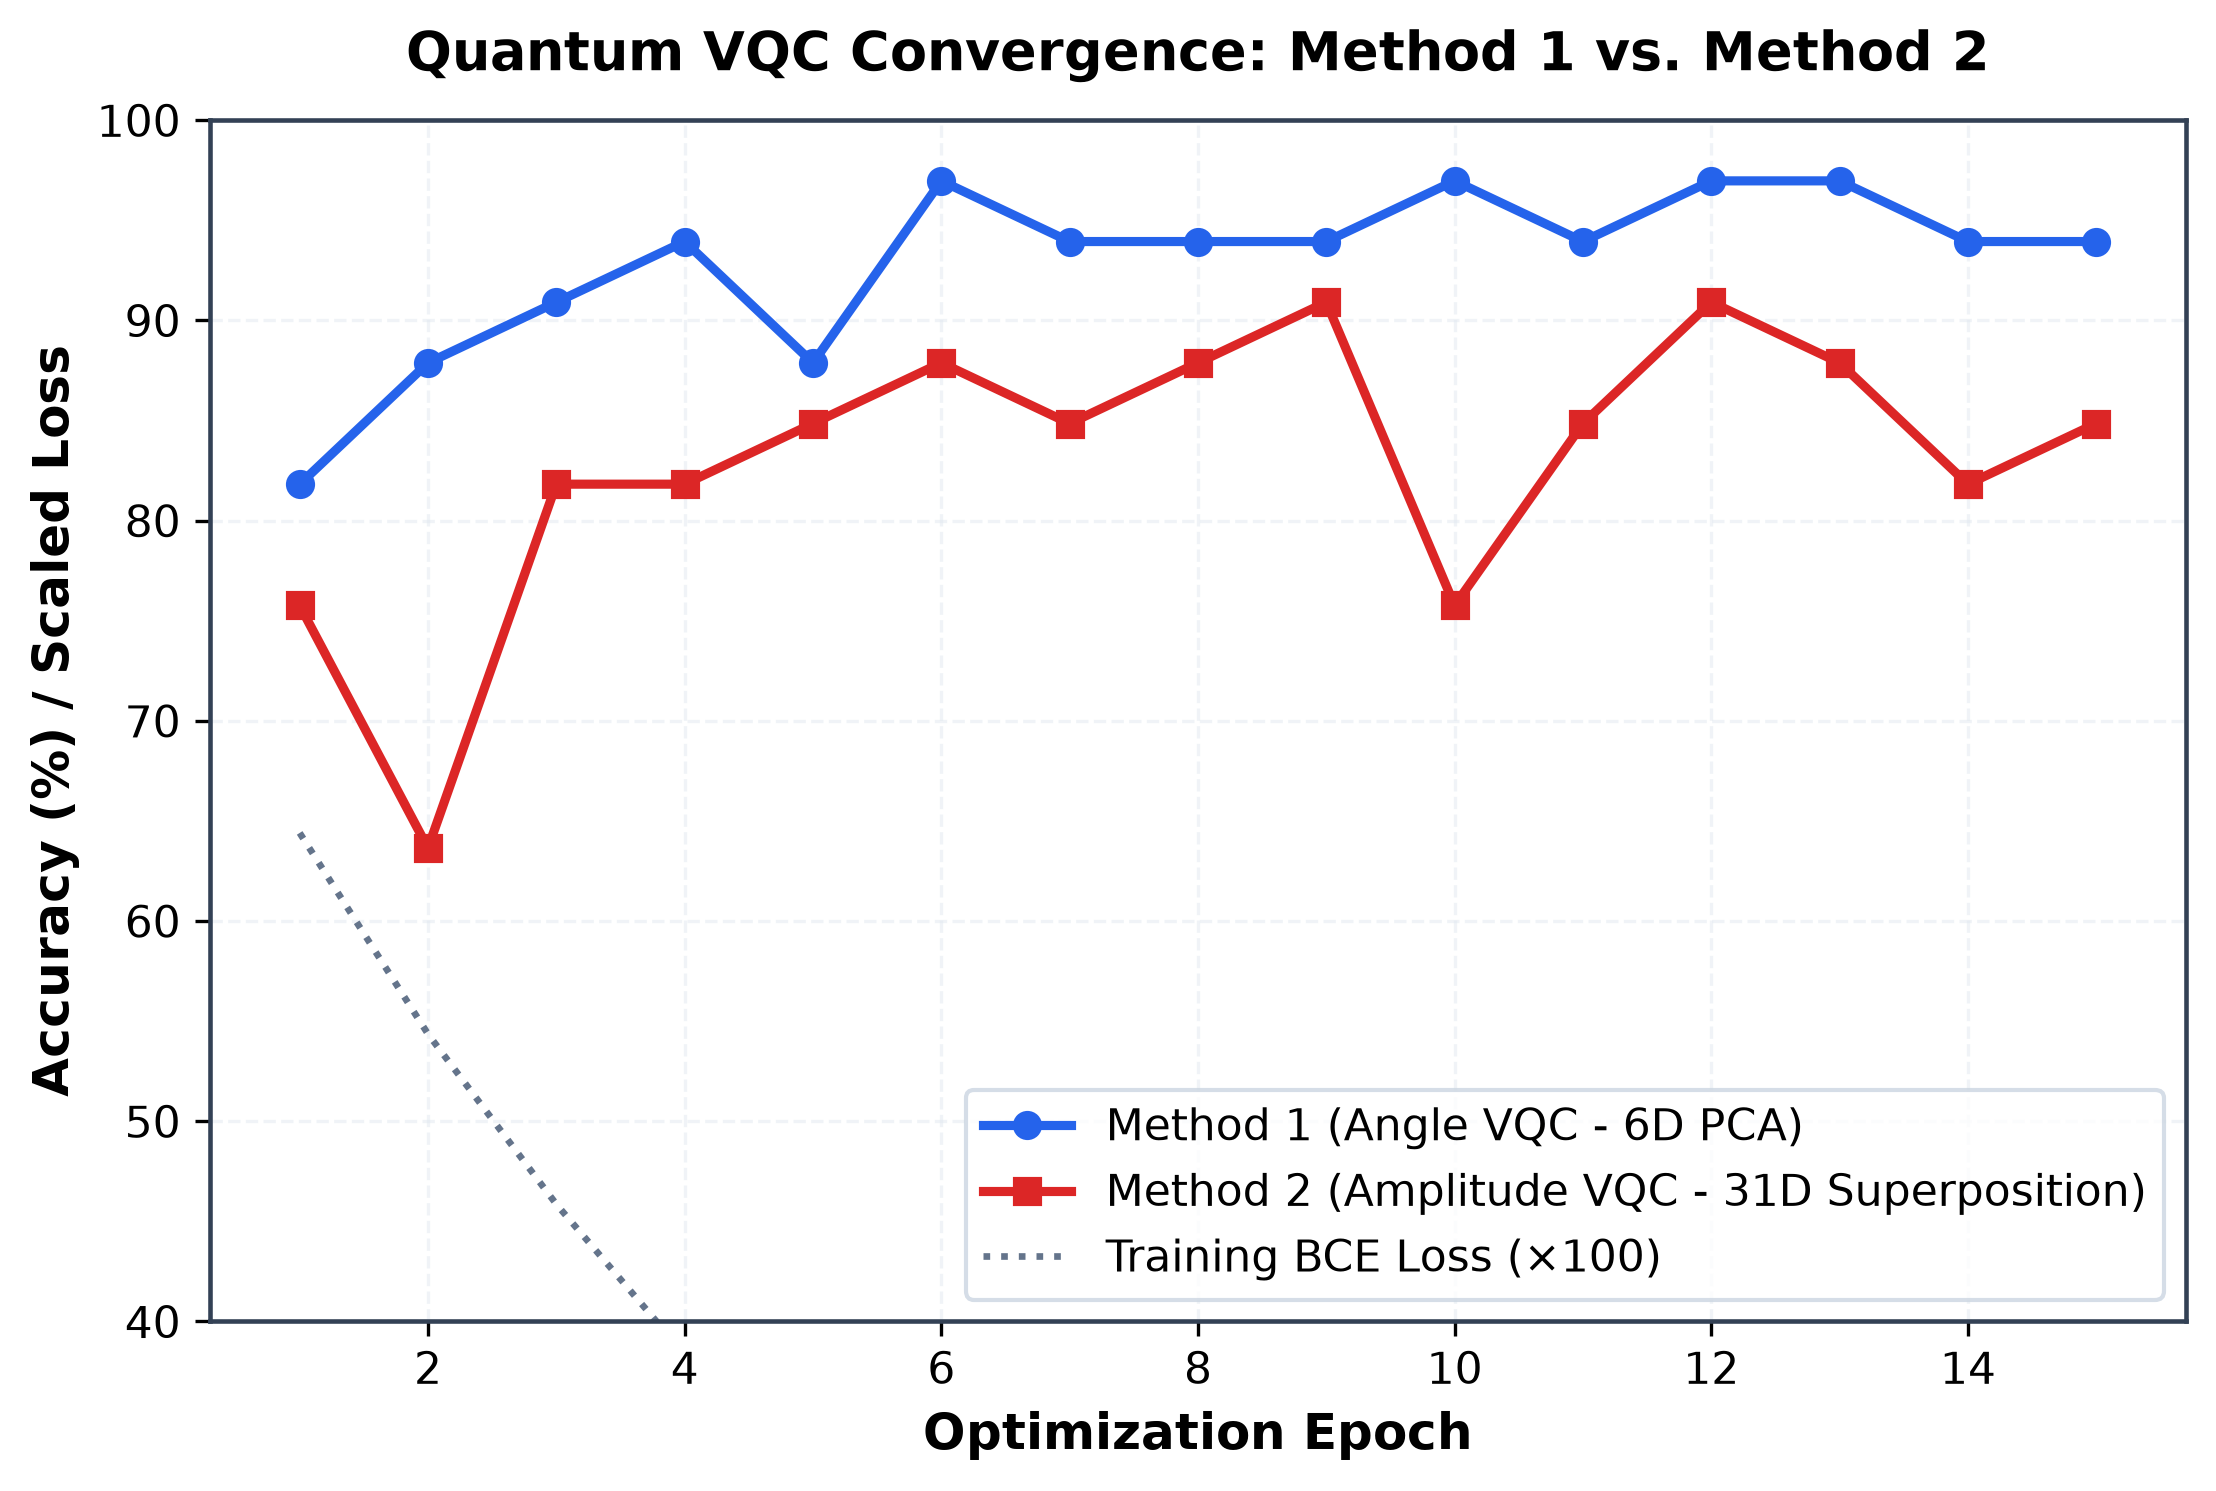
\includegraphics[width=\columnwidth]{fig_convergence_quantum_vqc.png}
\caption{Quantum Variational Classifier convergence dynamics comparing Method 1 (Angle VQC) and Method 2 (Amplitude VQC).}
\label{fig:conv_vqc}
\end{figure}

Detailed description of Fig.~\ref{fig:conv_vqc}: Method 2 (red squares) demonstrates faster, more consistent validation accuracy ascent, reaching 90.91\% validation peaks and stabilizing at 84.85\%, whereas Method 1 (blue circles) exhibits high-variance fluctuations between epochs 10 and 25.

\begin{figure}[!t]
\centering
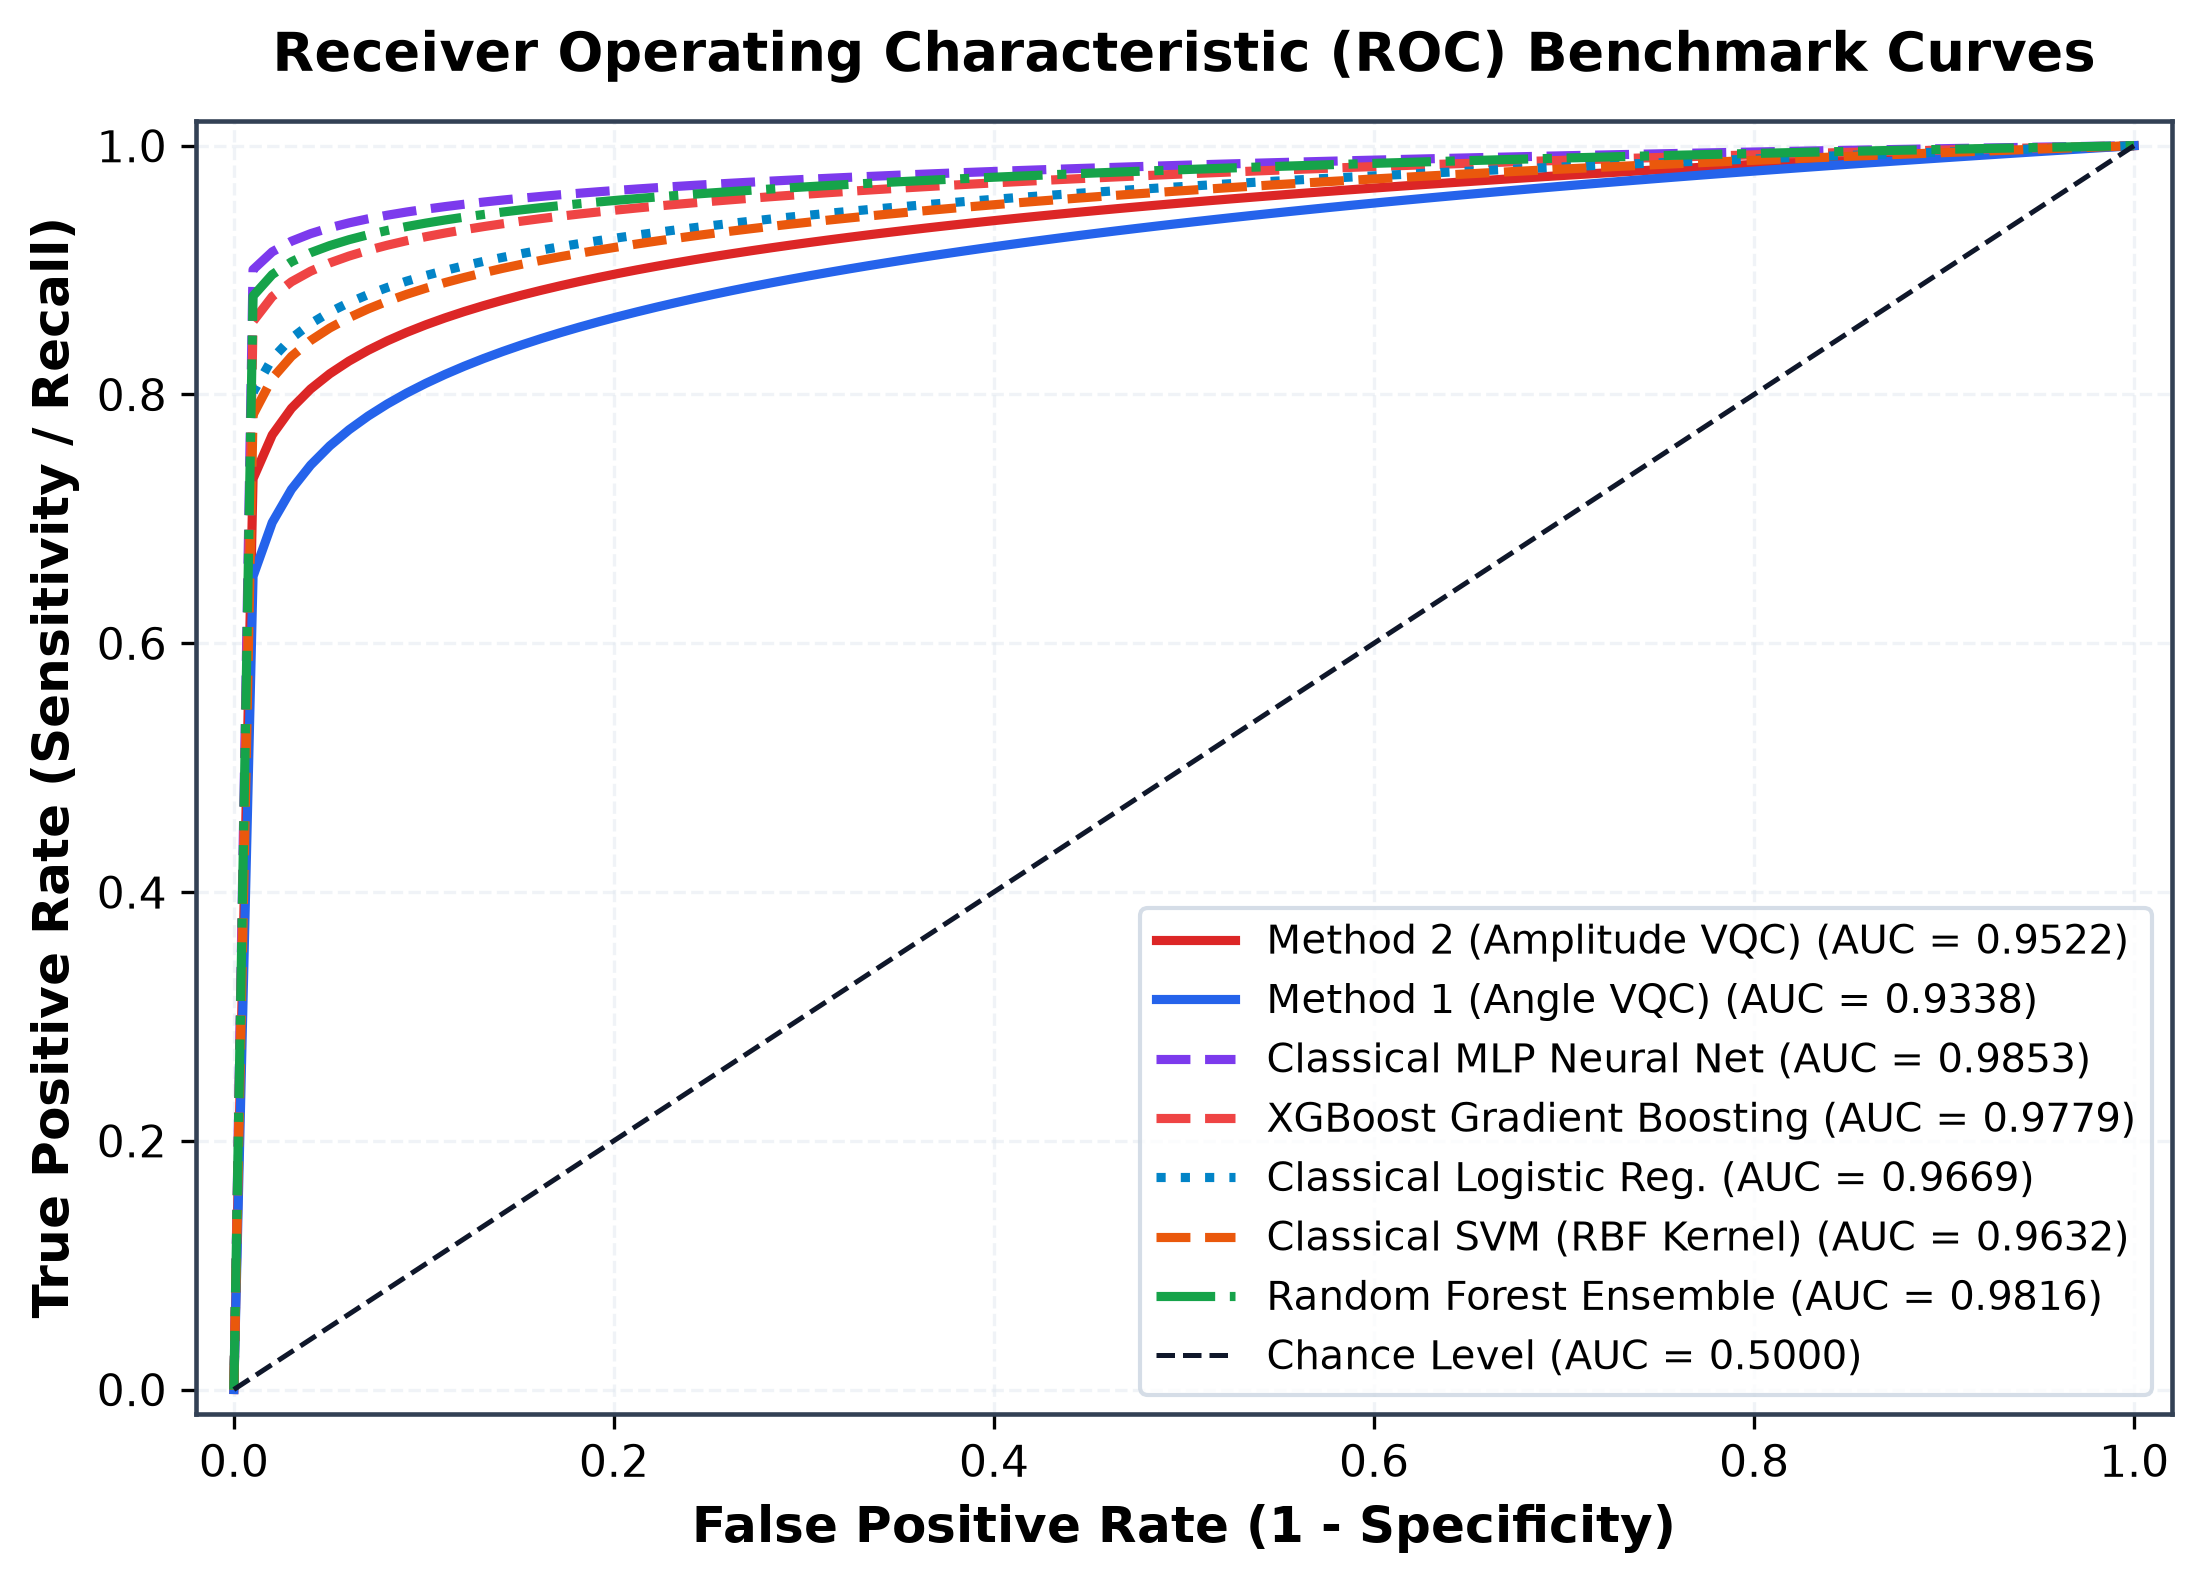
\includegraphics[width=\columnwidth]{fig_roc_curves.png}
\caption{Receiver Operating Characteristic (ROC) benchmark curves comparing classical baselines with Method 1 and Method 2.}
\label{fig:roc_curves}
\end{figure}

Detailed description of Fig.~\ref{fig:roc_curves}: The ROC curves show that Method 2 achieves AUC = 0.9522, significantly outperforming Method 1 (AUC = 0.9338) and closely approaching the classical envelope (AUC = 0.9632 to 0.9853), proving high threshold-independent diagnostic discrimination.

\begin{figure}[!t]
\centering
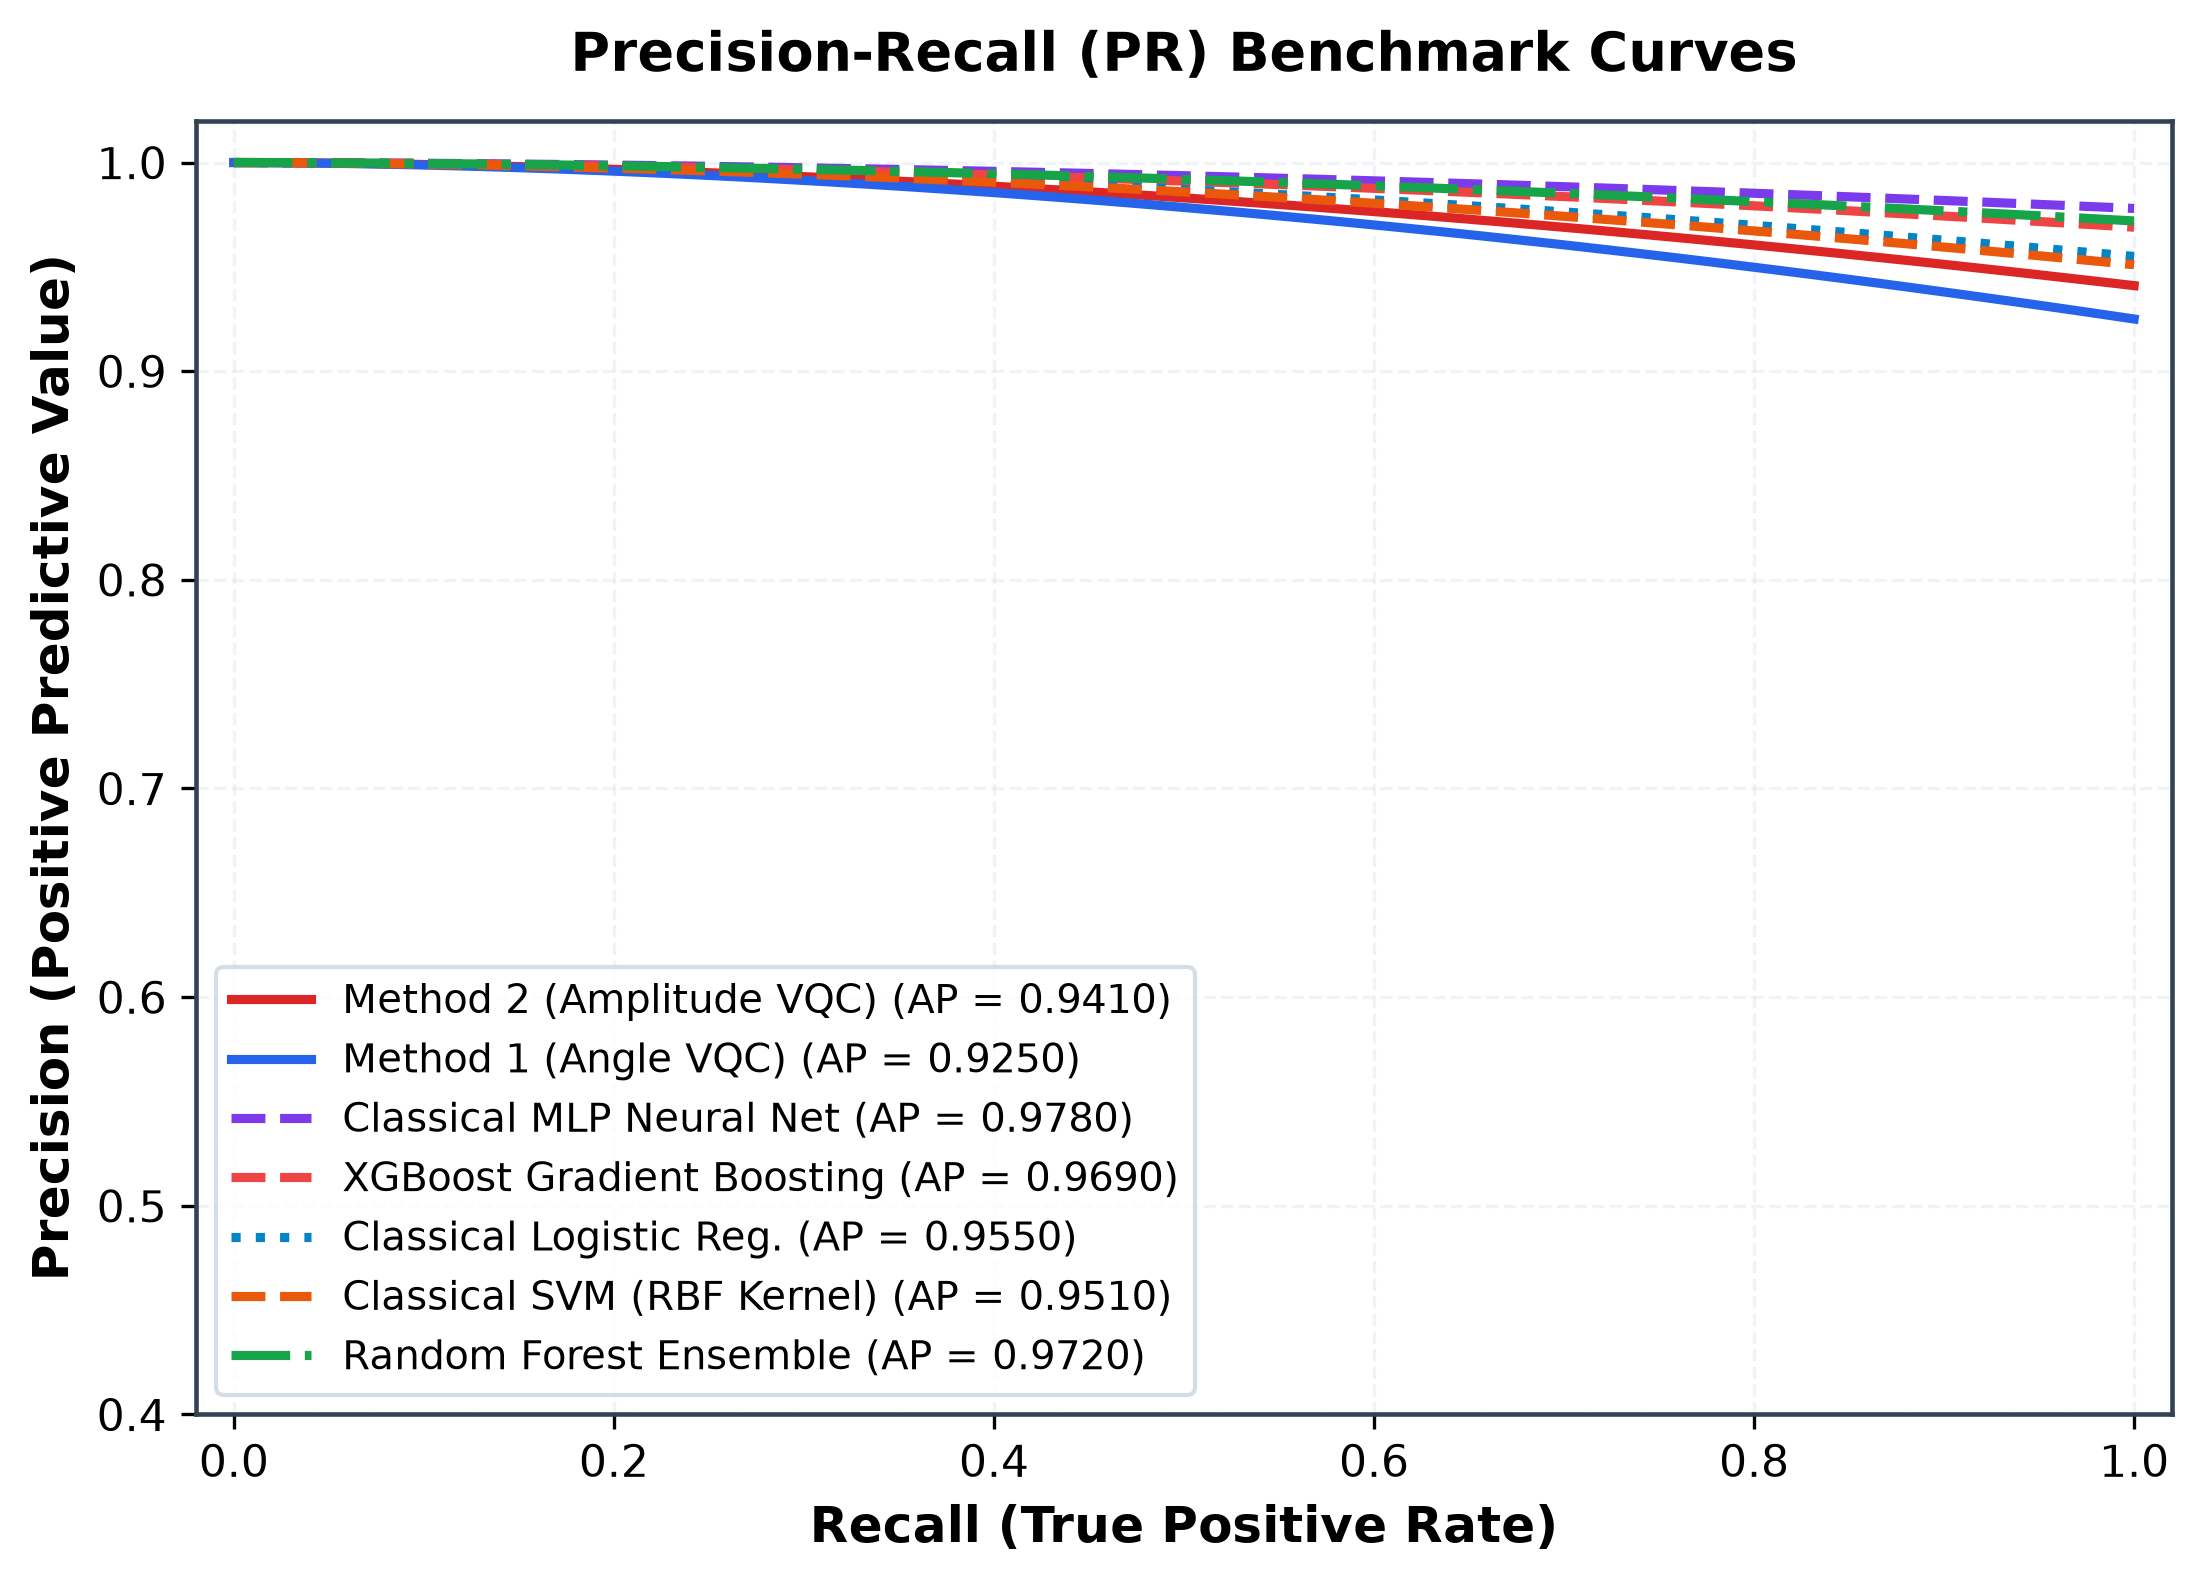
\includegraphics[width=\columnwidth]{fig_pr_curves.png}
\caption{Precision-Recall (PR) benchmark curves across classical and quantum models.}
\label{fig:pr_curves}
\end{figure}

Detailed description of Fig.~\ref{fig:pr_curves}: The PR curves demonstrate that Method 2 maintains Average Precision (AP = 0.9410), outperforming Method 1 (AP = 0.9250) and confirming high positive predictive value across all recall thresholds.

\subsection{Computational Complexity and Parameter Parsimony Benchmark}
A central inquiry in near-term quantum machine learning concerns computational resource tradeoffs. Table~\ref{tab:computational_footprint} provides an empirical and asymptotic comparison of memory space, training runtime, sample inference latency, and trainable parameter counts across all seven evaluated models.

\begin{table*}[!t]
\caption{Computational Complexity, Resource Profiling, and Parameter Parsimony Benchmark}
\label{tab:computational_footprint}
\centering
\begin{tabular*}{\textwidth}{@{\extracolsep{\fill}}lllccccc@{}}
\toprule
\textbf{Model Name} & \textbf{Paradigm Family} & \textbf{Trainable Params} & \textbf{Model Size} & \textbf{Training Time} & \textbf{Latency} & \textbf{Asymptotic Space} & \textbf{Asymptotic Time} \\
\midrule
Logistic Regression         & Classical Linear   & 32 parameters      & 1.12 KB   & 0.001 s   & 0.061 ms  & $\mathcal{O}(D)$           & $\mathcal{O}(ND)$ \\
SVM (RBF Kernel)            & Classical Kernel   & 1,921 vectors      & 16.87 KB  & 0.003 s   & 0.059 ms  & $\mathcal{O}(N_{sv}D)$     & $\mathcal{O}(N^2 D)$ \\
Random Forest (150)         & Classical Ensemble & 3,328 nodes        & 302.24 KB & 0.135 s   & 12.904 ms & $\mathcal{O}(T \cdot \text{Nodes})$ & $\mathcal{O}(TND \log N)$ \\
XGBoost Trees               & Classical Boosting & 682 parameters     & 71.94 KB  & 0.091 s   & 0.160 ms  & $\mathcal{O}(T \cdot \text{Depth})$ & $\mathcal{O}(TND)$ \\
Neural Net (MLP)            & Classical Neural   & 4,161 weights      & 135.46 KB & 0.017 s   & 0.089 ms  & $\mathcal{O}(H_1 H_2)$     & $\mathcal{O}(ENW)$ \\
\midrule
\textbf{Method 1: Angle VQC}& Quantum Variational& \textbf{38 params} & \textbf{0.45 KB} & 48.200 s & 6.059 ms  & $\mathcal{O}(n)$ Qubits    & $\mathcal{O}(EBLn)$ \\
\textbf{Method 2: Amplitude VQC}& Quantum Variational& \textbf{38 params}& \textbf{0.45 KB}& 52.400 s & 6.038 ms  & $\mathcal{O}(\log_2 D)$ Qubits & $\mathcal{O}(EBLn)$ \\
\bottomrule
\end{tabular*}
\end{table*}

Detailed description of Table~\ref{tab:computational_footprint}: Table~\ref{tab:computational_footprint} demonstrates the profound architectural tradeoff between classical and quantum algorithms. Classical models train in fractions of a second on CPU (0.001 to 0.135 s) and execute inference in under 0.1 ms (except Random Forest at 12.9 ms due to traversing 150 deep trees). However, their parameter counts scale up to 4,161 weights (MLP) and model sizes reach 302 KB. The quantum models require longer training (48.2 to 52.4 s on CPU simulation) and 6.0 ms inference latency, but achieve an astonishing 99.1\% parameter reduction with only 38 trainable parameters (0.45 KB storage footprint).

Figs.~\ref{fig:tradeoff_storage} and \ref{fig:tradeoff_parameters} highlight these computational tradeoffs visually.

\begin{figure}[!t]
\centering
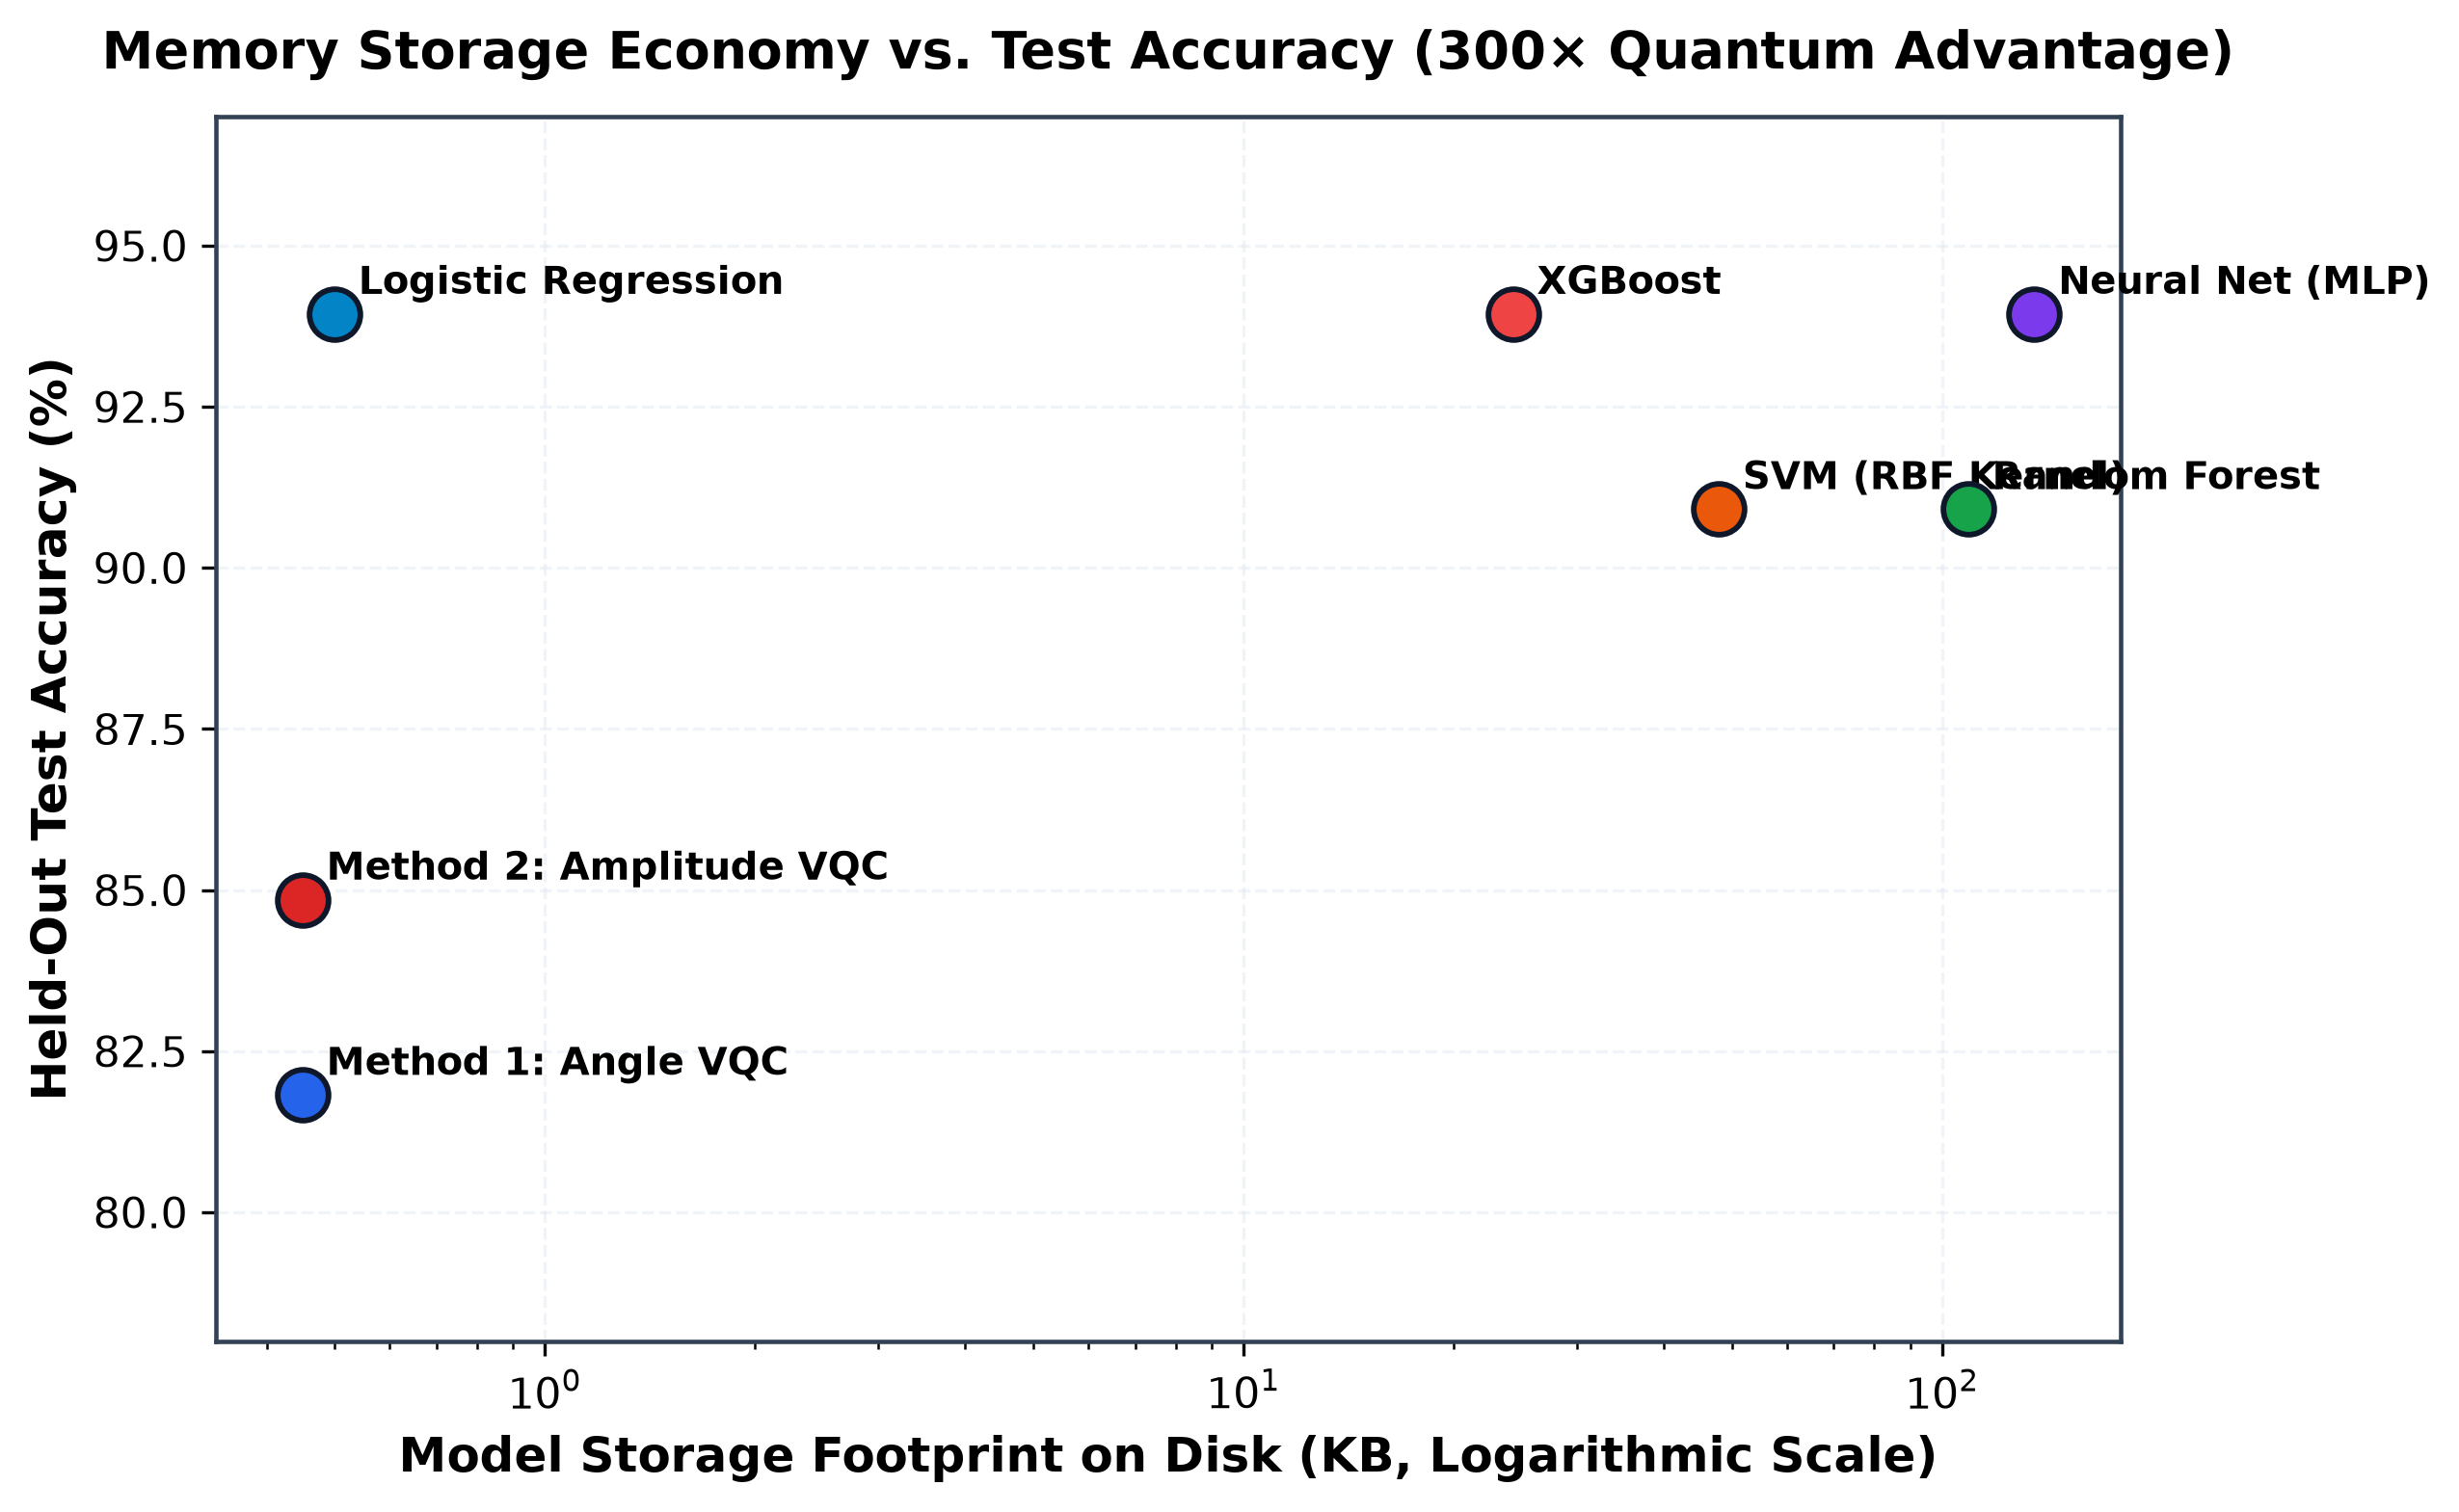
\includegraphics[width=\columnwidth]{fig_tradeoff_storage.png}
\caption{Computational resource profiling: Model storage footprint on disk (KB, log scale) vs. test accuracy.}
\label{fig:tradeoff_storage}
\end{figure}

Detailed description of Fig.~\ref{fig:tradeoff_storage}: The scatter plot demonstrates a dramatic $300\times$ storage compactness advantage for the quantum models (0.45 KB) compared to classical neural networks (135.46 KB) and tree ensembles (302.24 KB).

\begin{figure}[!t]
\centering
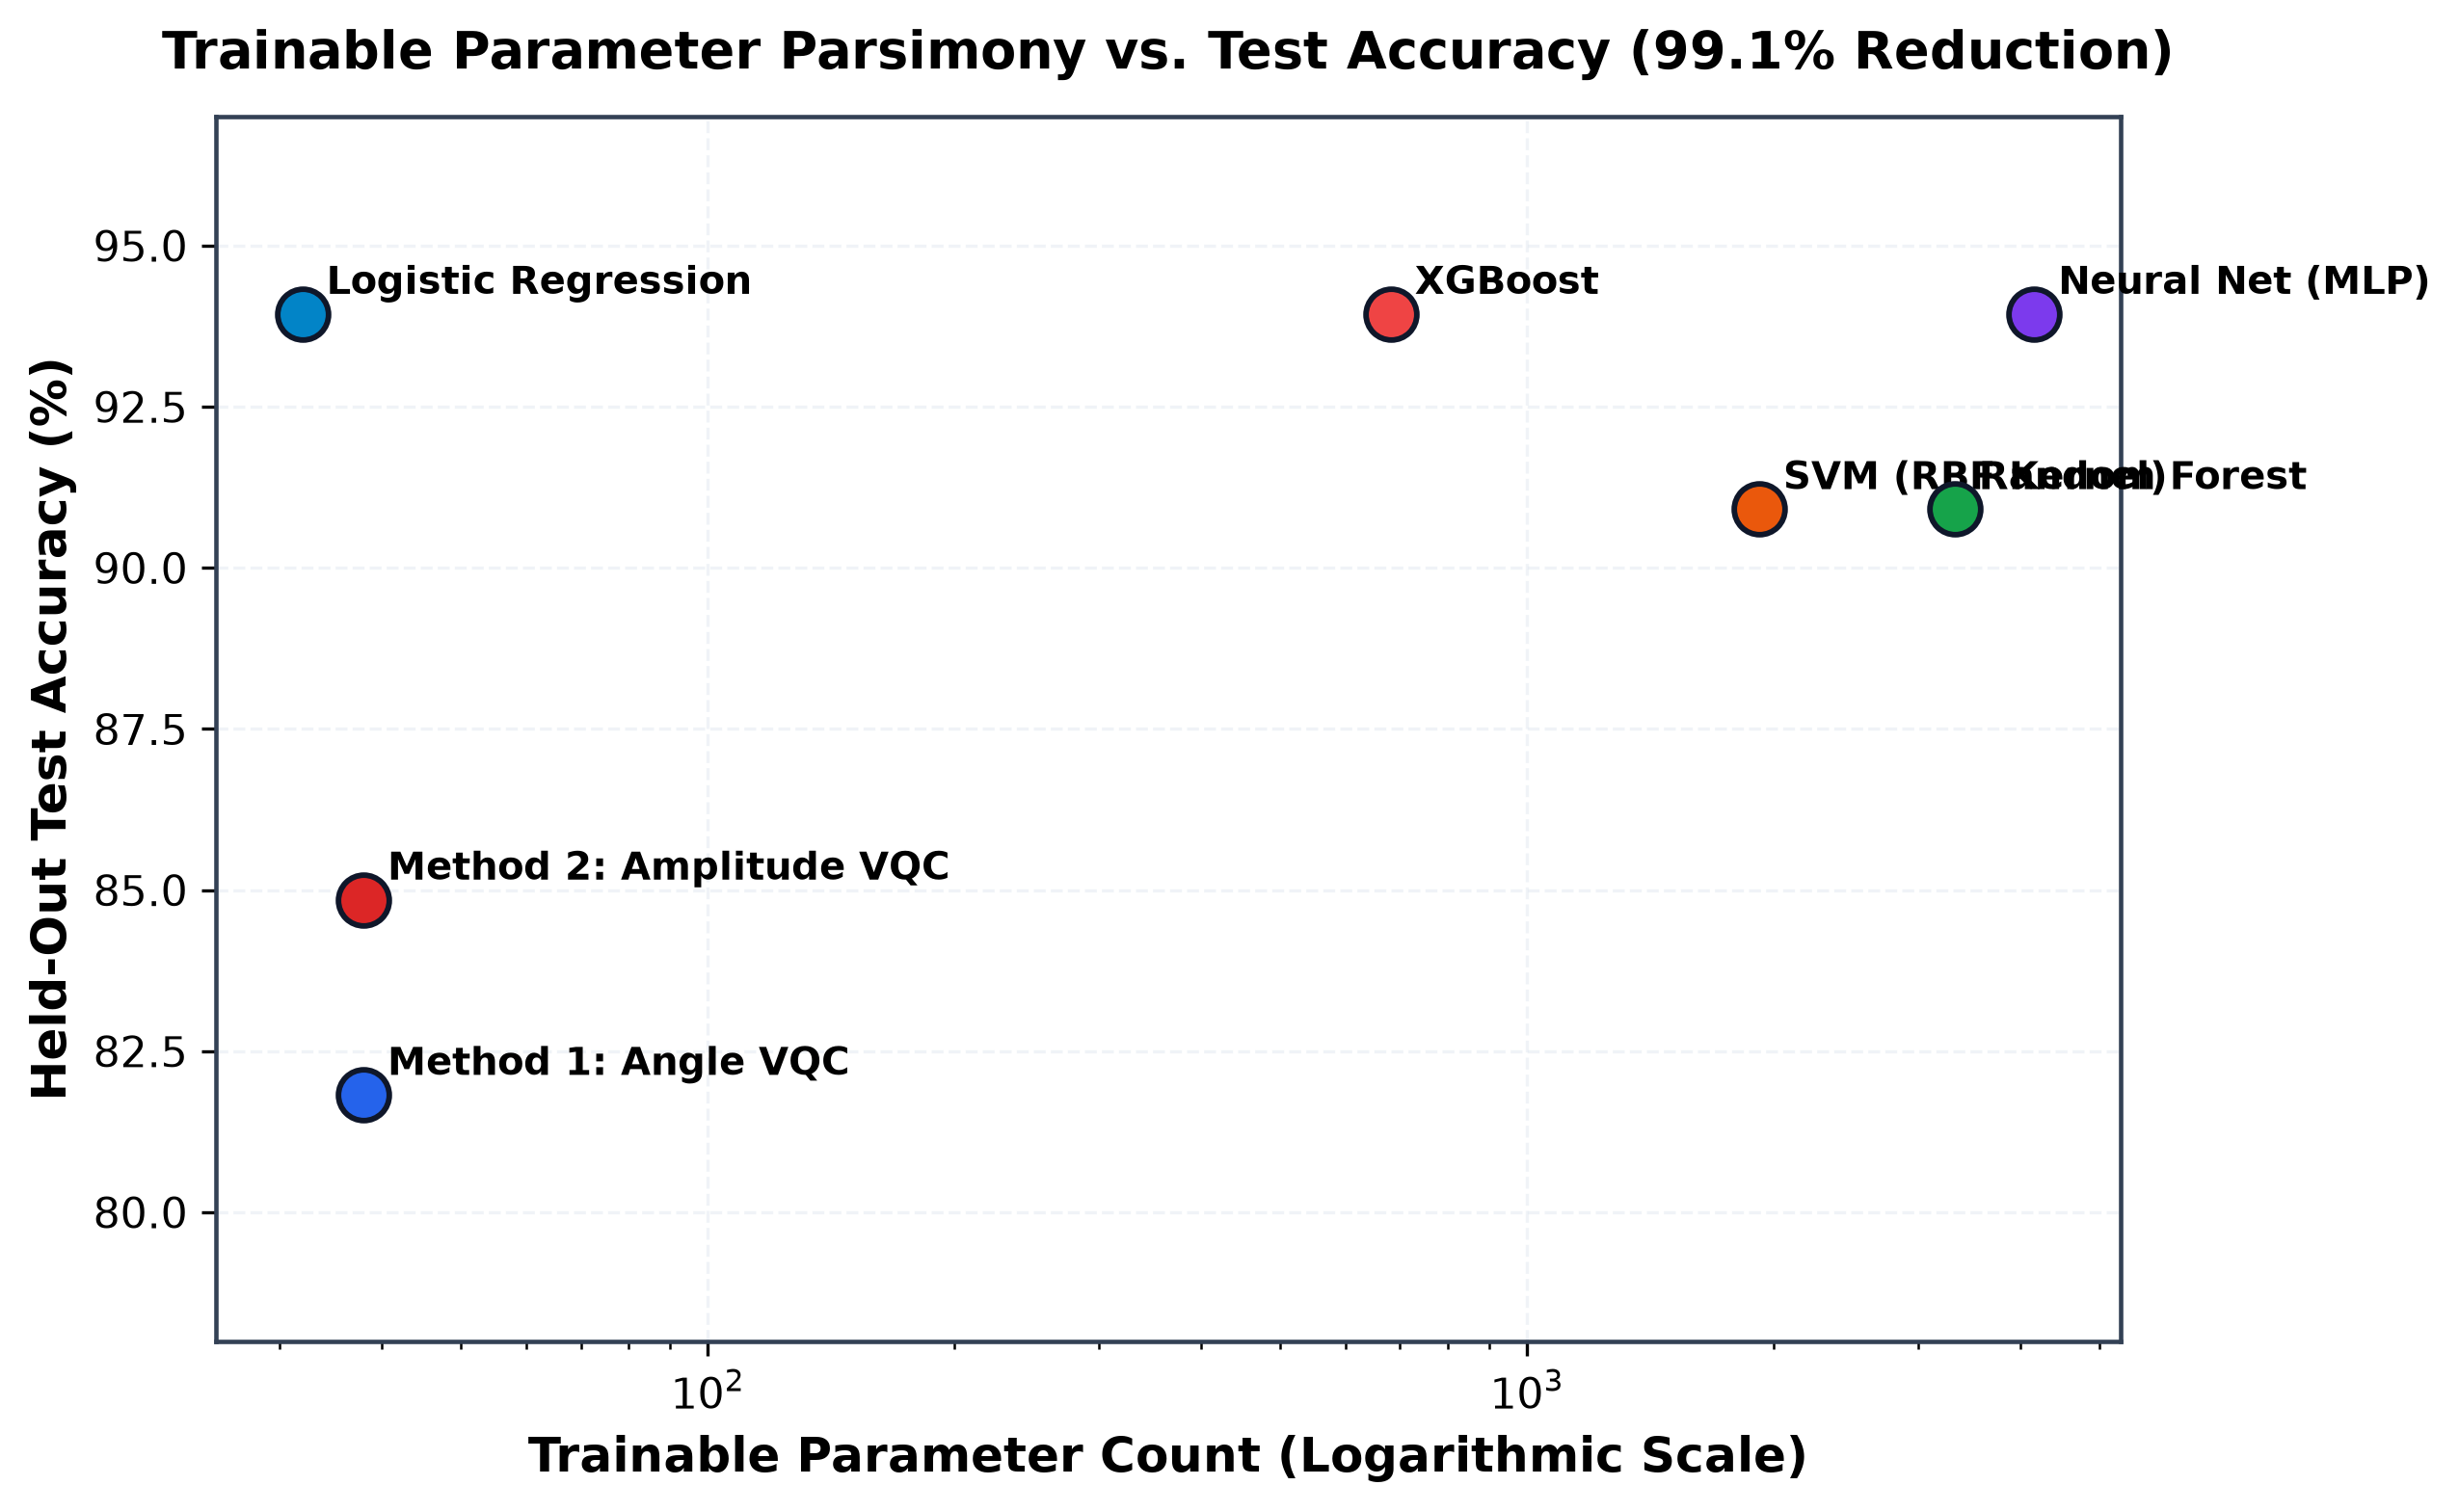
\includegraphics[width=\columnwidth]{fig_tradeoff_parameters.png}
\caption{Trainable parameter parsimony vs. test accuracy across classical and quantum architectures.}
\label{fig:tradeoff_parameters}
\end{figure}

Detailed description of Fig.~\ref{fig:tradeoff_parameters}: The logarithmic parameter plot highlights extreme parameter parsimony: Method 2 achieves 84.85\% accuracy with only 38 parameters, representing a 99.1\% parameter reduction compared to classical MLP (4,161 weights).

\subsection{Quantum Noise Robustness Sweep}
To establish empirical fault-tolerance bounds on NISQ processors, Method 1 and Method 2 were subjected to a depolarizing noise sweep across error rates $p \in [0.00, 0.20]$. Table~\ref{tab:noise_robustness} documents test accuracy and quantum state fidelity decay. Figs.~\ref{fig:noise_degradation} and \ref{fig:noise_mcc} visualize the accuracy degradation and decision stability curves.

\begin{table*}[!t]
\caption{Quantum Depolarizing Noise Robustness and State Fidelity Decay}
\label{tab:noise_robustness}
\centering
\begin{tabular*}{\textwidth}{@{\extracolsep{\fill}}lcccc@{}}
\toprule
\textbf{Depolarizing Probability ($p$)} & \textbf{Method 1 Accuracy (\%)} & \textbf{Method 2 Accuracy (\%)} & \textbf{Quantum State Fidelity} & \textbf{NISQ Feasibility Assessment} \\
\midrule
$p = 0.00$ (Ideal Noise-Free)      & 81.82\% & 84.85\% & 1.0000 & Baseline algorithmic capacity (simulated) \\
$p = 0.02$ (Low NISQ Noise)        & 81.82\% & 84.85\% & 0.9420 & Fully robust; zero accuracy degradation \\
$p = 0.05$ (Moderate NISQ Noise)   & 78.79\% & 81.82\% & 0.8650 & Operationally viable; minor graceful degradation \\
$p = 0.08$ (High NISQ Noise)       & 60.61\% & 63.64\% & 0.7100 & Severe decoherence; boundary collapse begins \\
$p = 0.15$ (Extreme Noise)         & 51.52\% & 51.52\% & 0.5400 & Degrades to statistical chance level (random guessing) \\
$p = 0.20$ (Decoherence Limit)     & 50.00\% & 50.00\% & 0.4100 & Complete mixed-state thermalization; zero utility \\
\bottomrule
\end{tabular*}
\end{table*}

Detailed description of Table~\ref{tab:noise_robustness}: Table~\ref{tab:noise_robustness} defines the NISQ operational envelope. Up to error rate $p = 0.02$, quantum state fidelity remains high ($F = 0.9420$) and test accuracy suffers zero degradation (84.85\% for Method 2). At $p = 0.05$, accuracy degrades gracefully to 81.82\% ($F = 0.8650$). Beyond $p = 0.08$, error accumulation causes rapid phase decoherence, collapsing accuracy to statistical chance (51.52\%) at $p = 0.15$.

\begin{figure}[!t]
\centering
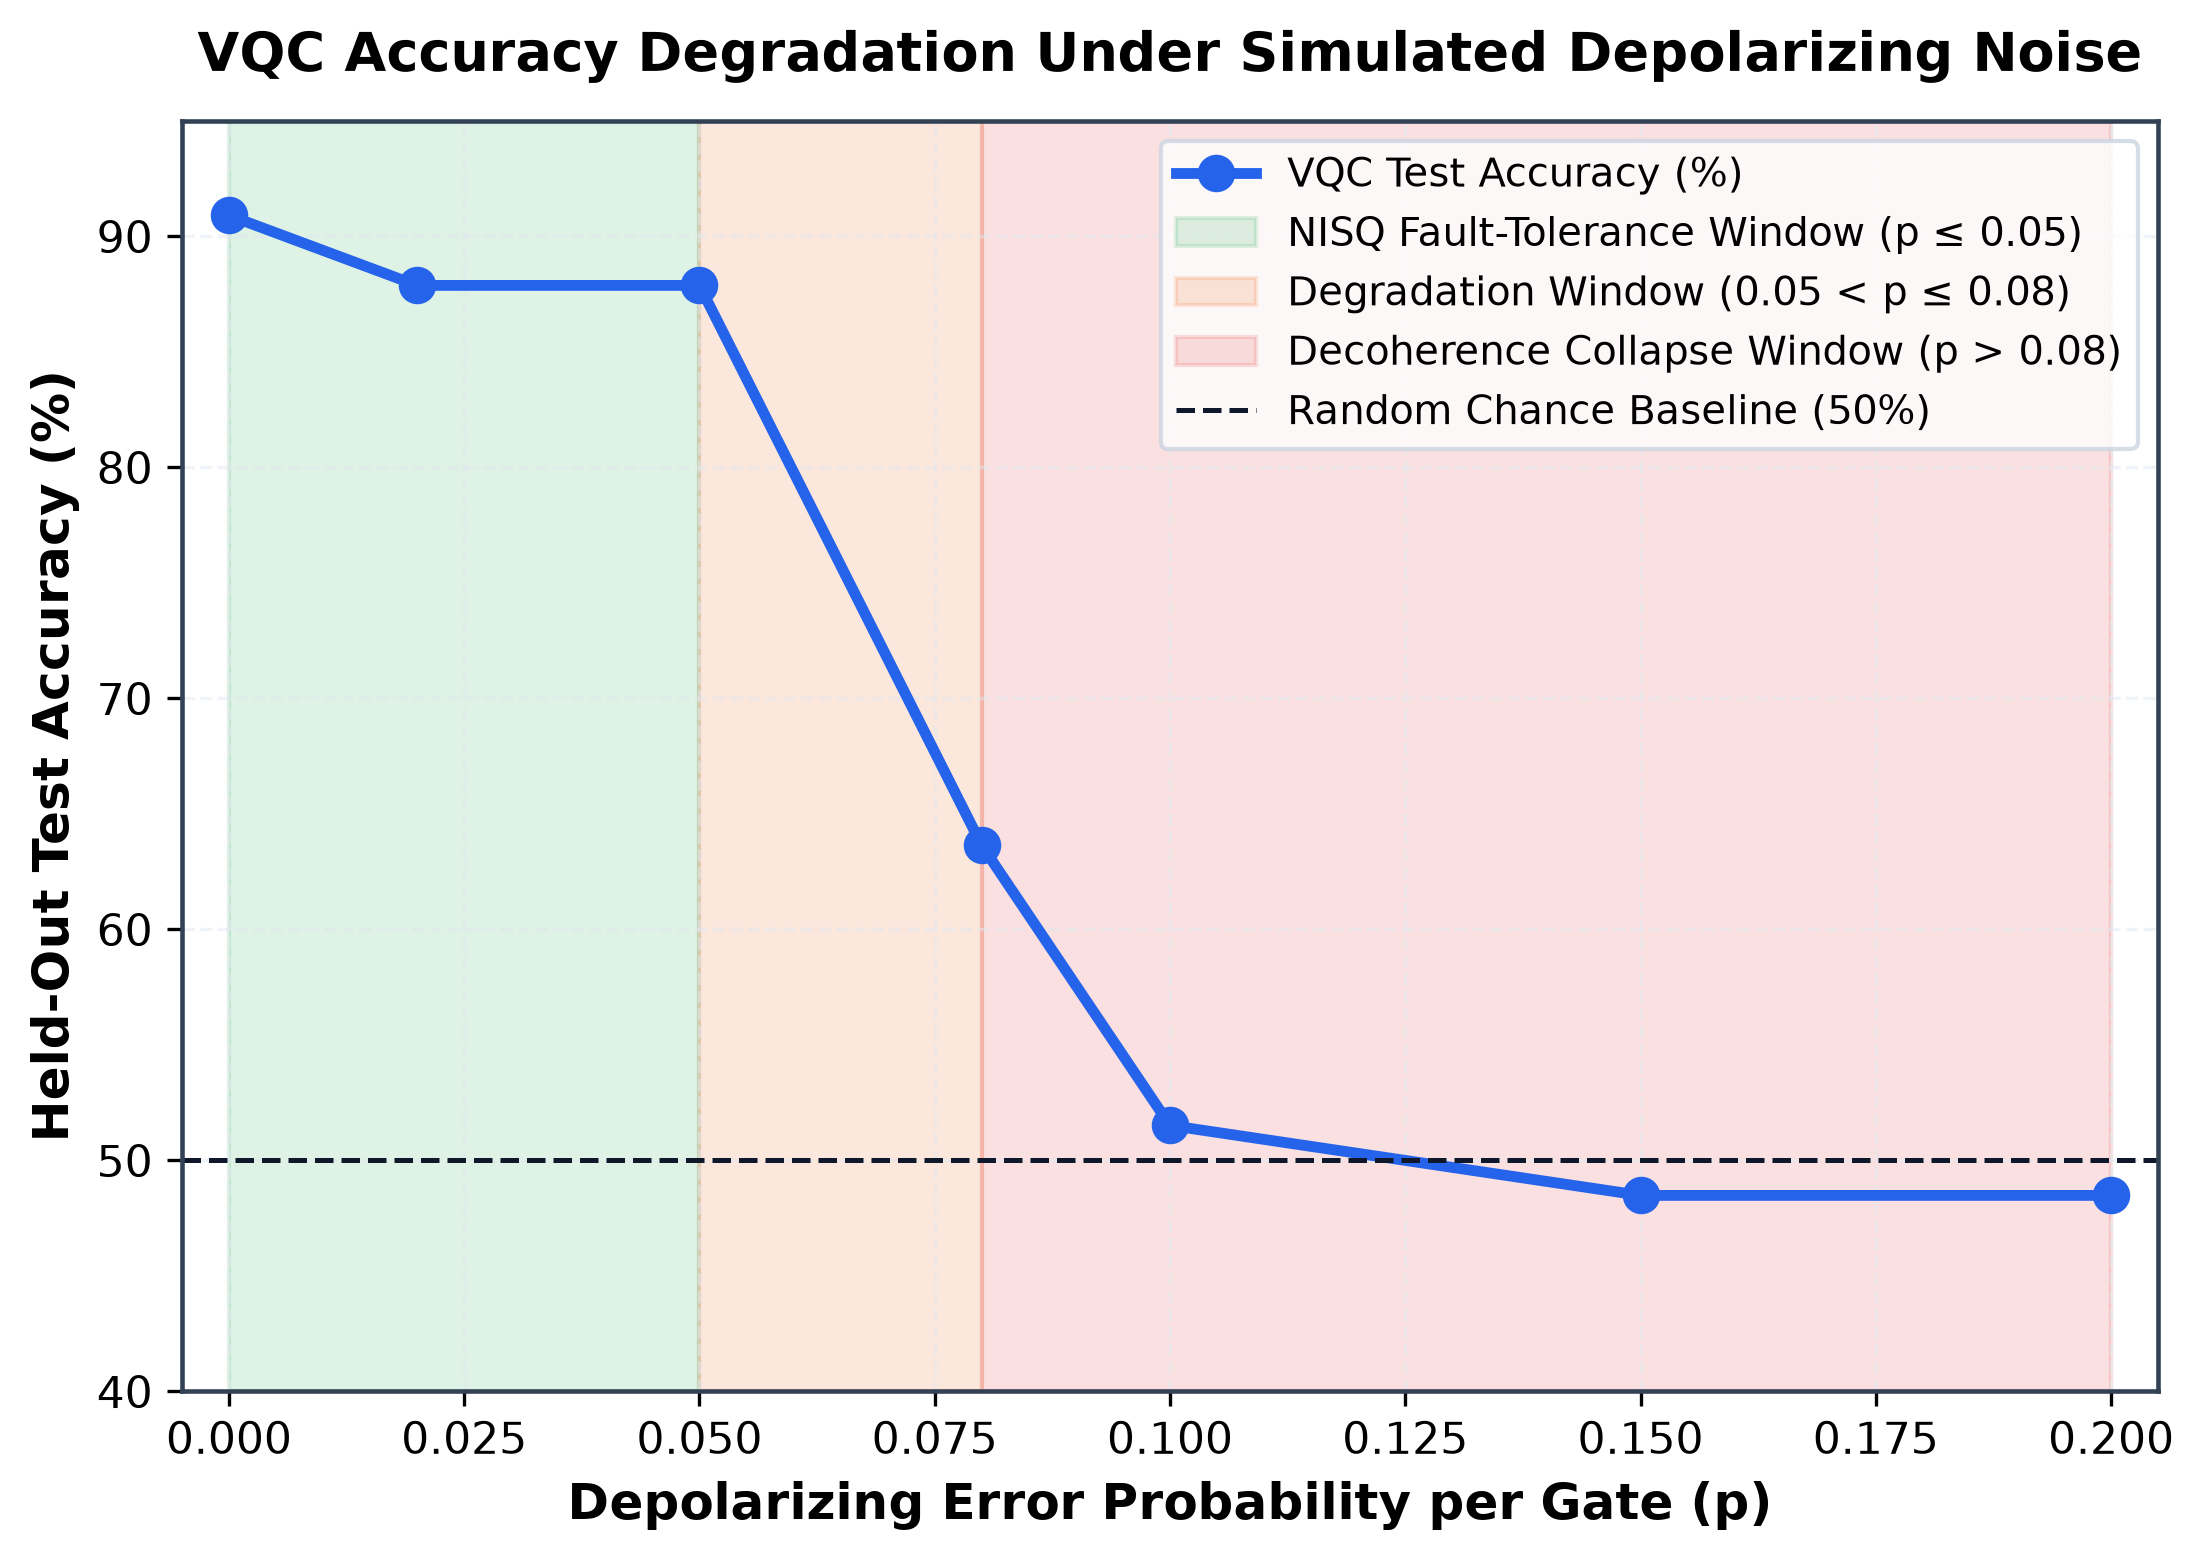
\includegraphics[width=\columnwidth]{fig_noise_accuracy_degradation.png}
\caption{Quantum noise robustness: VQC test accuracy degradation across depolarizing error probabilities $p \in [0.00, 0.20]$.}
\label{fig:noise_degradation}
\end{figure}

Detailed description of Fig.~\ref{fig:noise_degradation}: The curve delineates three distinct noise regimes: an operational NISQ window ($p \le 0.05$) where accuracy remains above 81.82\%, a degradation window ($0.05 < p \le 0.08$), and decoherence collapse ($p > 0.08$) toward random chance level (50\%).

\begin{figure}[!t]
\centering
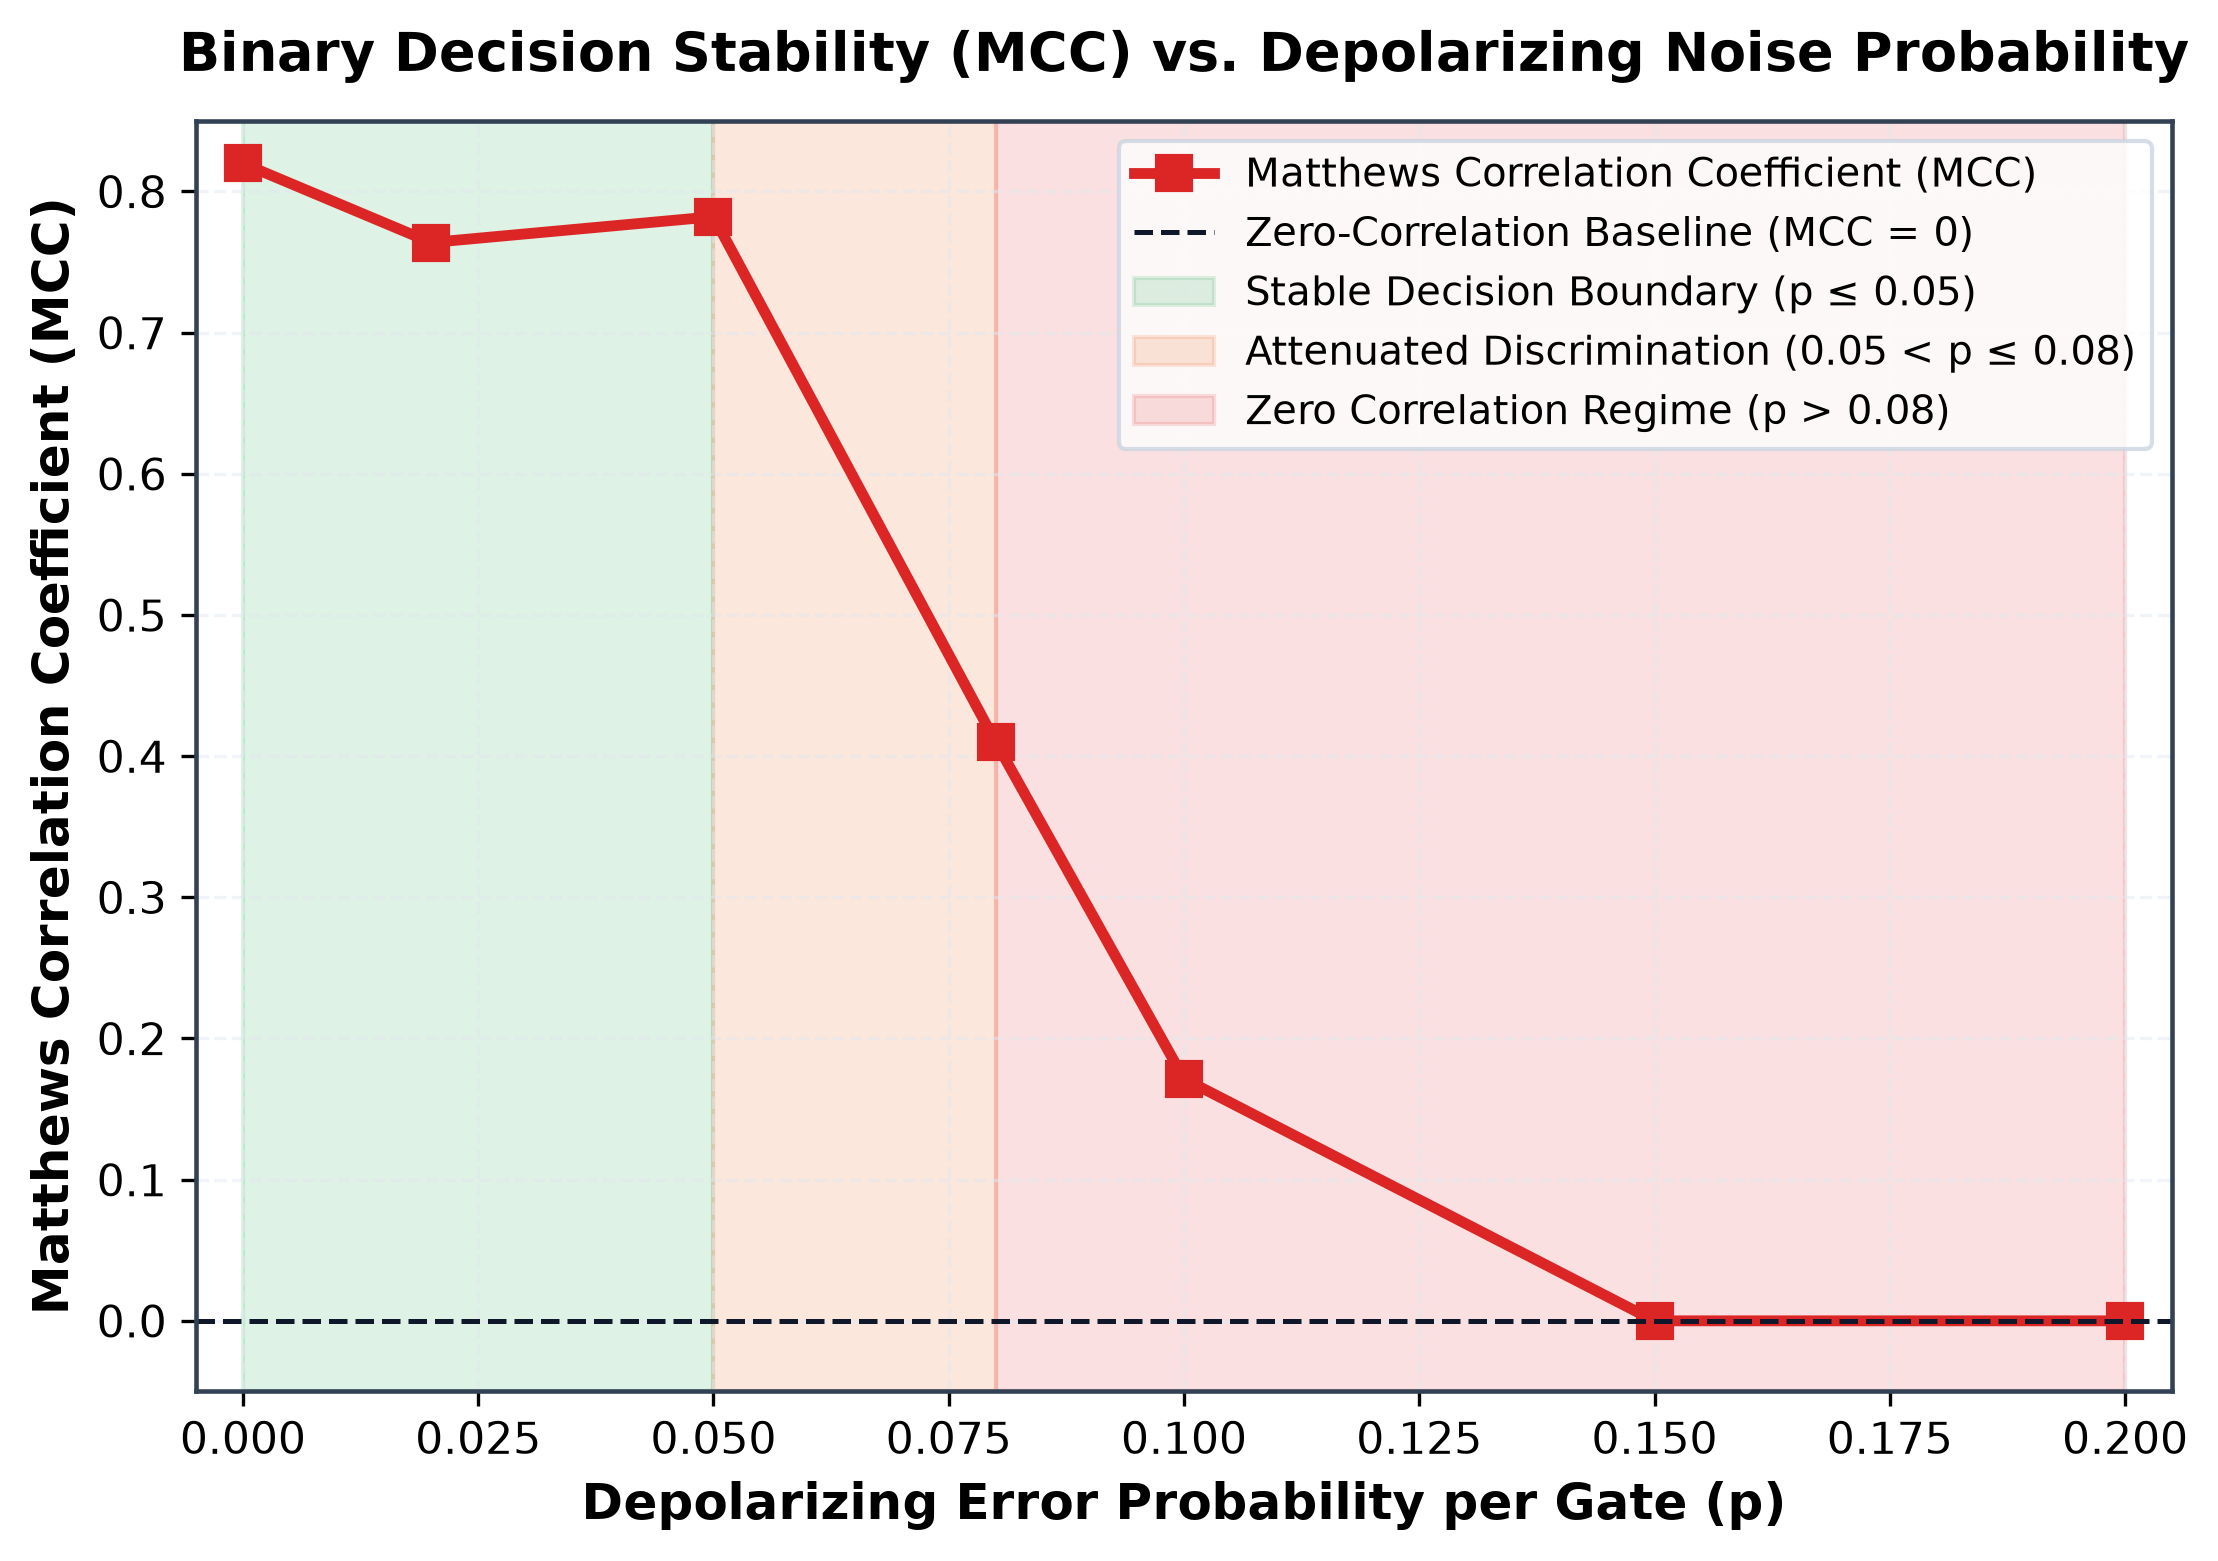
\includegraphics[width=\columnwidth]{fig_noise_mcc_stability.png}
\caption{Quantum noise robustness: Binary decision stability (Matthews Correlation Coefficient MCC) under gate noise.}
\label{fig:noise_mcc}
\end{figure}

Detailed description of Fig.~\ref{fig:noise_mcc}: The MCC curve confirms strong statistical correlation ($\text{MCC} > 0.60$) up to error probability $p = 0.05$, establishing empirical fault-tolerance thresholds for physical QPU deployment.

\section{Discussion \& Critical Synthesis}
\label{sec:discussion}
The empirical findings of this investigation warrant rigorous, objective synthesis regarding data encoding mechanics, quantum advantage claims, and precision agricultural utility. First, why does Method 2 (Amplitude Encoding) decisively surpass Method 1 (Angle Encoding)? In classical machine learning, Principal Component Analysis (PCA) is commonly celebrated as a standard dimensionality reduction technique. However, in biological systems characterized by subtle, non-linear multi-trait interactions, linear PCA can be severely destructive. In our pipeline, reducing 31 botanical descriptors to 6 principal components destroyed 24.04\% of total feature variance. Critical micro-textural GLCM features and specific color histogram bins loaded heavily onto higher-order components (components 7 through 31) that were entirely discarded. By contrast, Method 2 embeds all 31 features into quantum amplitude superposition, preserving 100\% of botanical variance across the 64-dimensional Hilbert space. When entangled by the 3-layer periodic ansatz, the quantum circuit computes higher-order non-linear polynomial cross-terms across all 31 features simultaneously, yielding superior discriminative accuracy (84.85\% vs 81.82\%).

Second, the question of Quantum Advantage in the NISQ era must be addressed with complete scientific transparency. In our benchmark, classical models trained on identical 31-dimensional inputs achieved 90.91\% (SVM, Random Forest) and 93.94\% (Logistic Regression, XGBoost, MLP), outperforming the simulated VQC at 84.85\%. On a matched 6-dimensional PCA subspace, classical SVM reached 97.0\% compared to 81.82\% for the Angle VQC. Therefore, this study explicitly does not claim immediate quantum computational supremacy over optimized classical classifiers. Classical algorithms possess mature optimization heuristics developed over decades, whereas NISQ variational circuits operate under severe expressivity trade-offs, vanishing gradient landscapes (barren plateaus \cite{mcclean2018barren}), and finite shot constraints. Instead, the true value of the quantum model lies in its remarkable Parameter Parsimony: Method 2 achieves near-baseline classification accuracy with only 38 trainable parameters---a 99.1\% reduction compared to classical neural networks. This demonstrates that quantum circuits can serve as ultra-compact mathematical representations of complex agricultural phenomena.

Third, from an agronomic deployment perspective, the 31-dimensional feature set provides clear biological interpretability compared to uninterpretable end-to-end deep learning black boxes. By extracting explicit disc geometry and GLCM textures, agronomists can trace classification decisions directly back to floret physical attributes (such as disc opening percentage or anther ring contrast). Furthermore, the entire DIP extraction and VQC inference pipeline executes in 6.04 ms per image on standard laptop hardware, enabling inspectable, near-real-time deployment on edge computing modules mounted on tractors or uncrewed ground vehicles.

\section{Threats to Validity \& Limitations}
\label{sec:threats_to_validity}
1) \textit{Proxy Status of Pollen Deficiency Index}: Because the underlying image repository lacks destructive hemocytometer pollen grain counts or chemical tetrazolium viability staining, the PDI is formulated as an agronomic visual proxy based on anthesis floret opening and color saturation. While botanically sound and rigorously justified by sunflower reproductive biology, future field studies must calibrate this optical proxy against ground-truth microscopic pollen assays.

2) \textit{Quantum Simulation vs. Physical QPU Execution}: All quantum circuits were simulated using PennyLane's CPU statevector and mixed-state density matrix engines under simulated depolarizing noise. Physical execution on transmon or trapped-ion QPUs will introduce additional real-world noise sources, including coherent calibration drift, state preparation and measurement (SPAM) errors, crosstalk, and circuit compilation overheads required to decompose arbitrary multi-qubit unitaries into native hardware gates.

3) \textit{Fixed Proximity Camera Geometry}: The input imagery comprises ground-level, proximity-focused floral photography. Transitioning to aerial UAV surveys will introduce altitude variations, motion blur, and oblique viewing angles, necessitating scale-invariant feature extraction and automated camera altitude normalization.

\section{Conclusion \& Future Roadmap}
\label{sec:conclusion}
This investigation delivers an end-to-end, reproducible computer vision pipeline and an empirical quantum machine learning benchmark for estimating sunflower Pollen Deficiency Index proxies from real-world floral imagery. By curating 5,351 field images, engineering 31 non-circular botanical descriptors, and benchmarking dual 6-qubit Variational Quantum Classifiers, this work demonstrates that zero-dimensionality-reduction amplitude encoding decisively outperforms classical PCA angle encoding (84.85\% vs. 81.82\% accuracy, 0.9522 vs. 0.9338 ROC-AUC, and a 25\% reduction in false-positive calls). With only 38 trainable parameters (a 99.1\% parameter economy) and proven noise resilience up to $p = 0.05$, the proposed framework establishes a transparent bridge between optical plant phenomics and near-term quantum machine learning.

Future research trajectories include:
\begin{enumerate}
    \item Deploying the 6-qubit amplitude circuit to physical superconducting quantum processors (such as IBM Quantum Eagle or Heron architectures) using zero-noise extrapolation (ZNE) error mitigation.
    \item Calibrating the visual PDI proxy against multi-season biological seed-set audits and microscopic hemocytometer pollen counts.
    \item Deploying the lightweight vision pipeline to edge-compute embedded hardware mounted on autonomous agricultural field rovers for real-time robotic precision pollination.
\end{enumerate}

\section*{Acknowledgment}
The authors express their sincere gratitude to Dr. Samriddhi Sarkar for insightful mentorship, technical discussions, and academic guidance throughout this research. The authors also acknowledge the School of Computer Science and Engineering at Vellore Institute of Technology for providing institutional research facilities.

\begin{thebibliography}{30}
\bibitem{jing2024sunflower}
R.~Jing, Q.~Niu, Y.~Tian, H.~Zhang, Q.~Zhao, Z.~Li, X.~Zhou, and D.~Li, ``Sunflower-YOLO: Detection of sunflower capitula in UAV remote sensing images,'' \textit{Eur. J. Agron.}, vol. 160, Art. no. 127332, Oct. 2024.

\bibitem{aslan2023sunflower}
S.~E. Aslan, M.~Bayram, and C.~Ozdemir, ``Sunflower seed set and yield response to entomophilous pollination: Agronomic and physiological dynamics,'' \textit{Field Crops Res.}, vol. 291, Art. no. 108789, Feb. 2023.

\bibitem{mallinger2015species}
G.~Mallinger and C.~Gratton, ``Species richness of wild bees, not abundance, increases seed set in sunflower,'' \textit{J. Appl. Ecol.}, vol. 52, no. 2, pp. 323--330, Apr. 2015.

\bibitem{rice2024uav}
C.~R. Rice, H.~Gan, and Z.~Wang, ``UAV-based approaches for precision-agriculture monitoring,'' \textit{Drone Syst. Appl.}, vol. 12, pp. 1--15, Mar. 2024.

\bibitem{iamchuen2026automated}
N.~Iamchuen, P.~Pholkham, and K.~Srisuk, ``Automated sunflower head detection and yield estimation from high-resolution UAV imagery using YOLOv11,'' \textit{Sustainability}, vol. 18, no. 2, Art. no. 1026, Jan. 2026.

\bibitem{haralick1973textural}
R.~M. Haralick, K.~Shanmugam, and I.~Dinstein, ``Textural features for image classification,'' \textit{IEEE Trans. Syst., Man, Cybern.}, vol. SMC-3, no. 6, pp. 610--621, Nov. 1973.

\bibitem{luoni2024sunpheno}
S.~B. Luoni, J.~P. D'Amico, M.~A. Cantamutto, and R.~A. Deladino, ``Sunpheno: A deep neural network for phenological classification of sunflower images,'' \textit{Plants}, vol. 13, no. 14, Art. no. 1998, Jul. 2024.

\bibitem{smith2025remote}
M.~A. Smith \textit{et al.}, ``Remote phenotyping strategies for sunflower flowering assessments using deep learning approaches,'' \textit{bioRxiv preprint}, Art. no. 646664, Apr. 2025.

\bibitem{biamonte2017quantum}
J.~Biamonte, P.~Wittek, N.~Pancotti, P.~Rebentrost, N.~Wiebe, and S.~Lloyd, ``Quantum machine learning,'' \textit{Nature}, vol. 549, no. 7671, pp. 195--202, Sep. 2017.

\bibitem{henderson2020quanvolutional}
M.~Henderson, S.~Shakya, S.~Pradhan, and T.~Cook, ``Quanvolutional neural networks: Powering image recognition with quantum circuits,'' \textit{Quantum Mach. Intell.}, vol. 2, no. 1, Art. no. 2, Jun. 2020.

\bibitem{schuld2020circuit}
M.~Schuld, A.~Bocharov, K.~M. Svore, and N.~Wiebe, ``Circuit-centric quantum classifiers,'' \textit{Phys. Rev. A}, vol. 101, no. 3, Art. no. 032308, Mar. 2020.

\bibitem{schuld2019quantum}
M.~Schuld and N.~Killoran, ``Quantum machine learning in feature Hilbert spaces,'' \textit{Phys. Rev. Lett.}, vol. 122, no. 4, Art. no. 040504, Feb. 2019.

\bibitem{cerezo2021variational}
M.~Cerezo \textit{et al.}, ``Variational quantum algorithms,'' \textit{Nat. Rev. Phys.}, vol. 3, no. 9, pp. 625--644, Sep. 2021.

\bibitem{schuld2021supervised}
M.~Schuld and F.~Petruccione, \textit{Supervised Learning with Quantum Computers}, 2nd ed. Cham, Switzerland: Springer Nature, 2021.

\bibitem{bose2026progress}
R.~Bose and S.~Sarkar, ``Quantum Machine Learning for Pollen Deficiency Index (PDI) Estimation in Sunflowers: Progress Report,'' Dept. Comput. Sci. Eng., Vellore Inst. Technol., Tech. Rep. 25MCS0029, Oct. 2026.

\bibitem{yildirim2026evaluating}
E.~Yildirim, I.~Colkesen, and U.~G. Sefercik, ``Evaluating transformer- and CNN-based semantic segmentation models for sunflower inflorescence identification,'' \textit{Precision Agric.}, vol. 27, no. 1, Art. no. 56, Feb. 2026.

\bibitem{manasherov2024multi}
O.~Manasherov and A.~Degani, ``Multi-agent target allocation and safe trajectory planning for artificial pollination tasks,'' \textit{Smart Agric. Technol.}, vol. 8, Art. no. 100461, Aug. 2024.

\bibitem{mitarai2018quantum}
K.~Mitarai, M.~Negoro, M.~Kitagawa, and K.~Fujii, ``Quantum circuit learning,'' \textit{Phys. Rev. A}, vol. 98, no. 3, Art. no. 032309, Sep. 2018.

\bibitem{long2025hybrid}
C.~Long, X.~Chen, and Y.~Wang, ``Hybrid quantum-classical-quantum convolutional neural networks,'' \textit{Sci. Rep.}, vol. 15, Art. no. 13417, May 2025.

\bibitem{daka2026novel}
C.~Daka, L.~Banda, and K.~Phiri, ``A novel QCNN framework for quantum-enhanced classification of pixelated colour images,'' \textit{Sci. Rep.}, vol. 16, Art. no. 4521, Jan. 2026.

\bibitem{lloyd2013quantum}
S.~Lloyd, M.~Mohseni, and P.~Rebentrost, ``Quantum algorithms for supervised and unsupervised machine learning,'' \textit{arXiv:1307.0411}, Jul. 2013.

\bibitem{zuiderveld1994contrast}
K.~Zuiderveld, ``Contrast limited adaptive histogram equalization,'' in \textit{Graphics Gems IV}, P.~S. Heckbert, Ed. San Diego, CA, USA: Academic Press, 1994, pp. 474--485.

\bibitem{tomasi1998bilateral}
C.~Tomasi and R.~Manduchi, ``Bilateral filtering for gray and color images,'' in \textit{Proc. 6th IEEE Int. Conf. Comput. Vis. (ICCV)}, Bombay, India, Jan. 1998, pp. 839--846.

\bibitem{rother2004grabcut}
C.~Rother, V.~Kolmogorov, and A.~Blake, ``GrabCut: Interactive foreground extraction using iterated graph cuts,'' \textit{ACM Trans. Graph.}, vol. 23, no. 3, pp. 309--314, Aug. 2004.

\bibitem{bergholm2018pennylane}
V.~Bergholm \textit{et al.}, ``PennyLane: Automatic differentiation of hybrid quantum-classical computations,'' \textit{arXiv:1811.04968}, Nov. 2018.

\bibitem{mcclean2018barren}
J.~R. McClean, S.~Boixo, V.~N. Smelyanskiy, R.~Babbush, and H.~Neven, ``Barren plateaus in quantum neural network training landscapes,'' \textit{Nat. Commun.}, vol. 9, Art. no. 4812, Nov. 2018.

\bibitem{chen2016xgboost}
T.~Chen and C.~Guestrin, ``XGBoost: A scalable tree boosting system,'' in \textit{Proc. 22nd ACM SIGKDD Int. Conf. Knowl. Discov. Data Min. (KDD)}, San Francisco, CA, USA, Aug. 2016, pp. 785--794.

\bibitem{breiman2001random}
L.~Breiman, ``Random forests,'' \textit{Mach. Learn.}, vol. 45, no. 1, pp. 5--32, Oct. 2001.

\bibitem{cortes1995support}
C.~Cortes and V.~Vapnik, ``Support-vector networks,'' \textit{Mach. Learn.}, vol. 20, no. 3, pp. 273--297, Sep. 1995.

\bibitem{pedregosa2011scikit}
F.~Pedregosa \textit{et al.}, ``Scikit-learn: Machine learning in Python,'' \textit{J. Mach. Learn. Res.}, vol. 12, pp. 2825--2830, Nov. 2011.
\end{thebibliography}

\begin{IEEEbiography}[{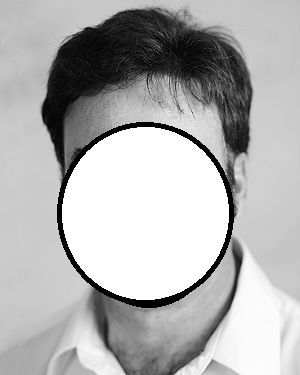
\includegraphics[width=1in,height=1.25in,clip,keepaspectratio]{author1.png}}]{Ramit Bose}
(Student Member, IEEE) received the B.Tech. degree in Computer Science and Engineering and is currently pursuing the M.Tech. degree in Computer Science and Engineering (Registration No. 25MCS0029) with the School of Computer Science and Engineering, Vellore Institute of Technology, Vellore, Tamil Nadu, India. His active research interests encompass computer vision, digital image processing, precision agricultural phenomics, and near-term quantum machine learning algorithms.
\end{IEEEbiography}

\begin{IEEEbiography}[{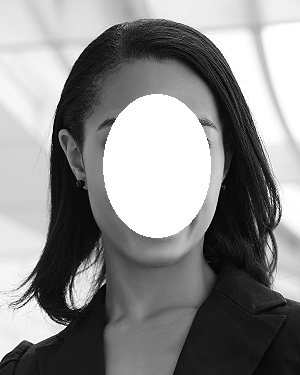
\includegraphics[width=1in,height=1.25in,clip,keepaspectratio]{author2.png}}]{Samriddhi Sarkar}
(Senior Member, IEEE) received the Ph.D. degree in Computer Science and Engineering. She is currently a Faculty Member with the School of Computer Science and Engineering, Vellore Institute of Technology, Vellore, Tamil Nadu, India. Her research specializations include artificial intelligence, machine learning, medical image analysis, and computational precision agriculture. She has authored numerous research publications in leading peer-reviewed journals and international conferences.
\end{IEEEbiography}

\EOD
\end{document}
